% !TeX root = memoria.tex
\documentclass[12pt]{report} % fuente a 12pt

% MÁRGENES: 2,5 cm sup. e inf.; 3 cm izdo. y dcho.
\usepackage[
a4paper,
vmargin=2cm,
hmargin=3cm
]{geometry}

% INTERLINEADO: Estrecho (6 ptos./interlineado 1,15) o Moderado (6 ptos./interlineado 1,5)
\renewcommand{\baselinestretch}{1.15}
\parskip=6pt

% DEFINICIÓN DE COLORES para portada y listados de código
\usepackage[table]{xcolor}
\definecolor{azulUC3M}{RGB}{0,0,102}
\definecolor{gray97}{gray}{.97}
\definecolor{gray75}{gray}{.75}
\definecolor{gray45}{gray}{.45}
\usepackage{enumitem}
% Soporte para GENERAR PDF/A --es importante de cara a su inclusión en e-Archivo porque es el formato óptimo de preservación y a la generación de metadatos, tal y como se describe en http://uc3m.libguides.com/ld.php?content_id=31389625. 

% En la plantilla incluimos el archivo OUTPUT.XMPDATA. Puedes descargar este archivo e incluir los metadatos que se incorporarán al archivo PDF cuando compiles el archivo memoria.tex. Después vuelve a subirlo a tu proyecto. 
\usepackage[a-1b]{pdfx}

% ENLACES
\usepackage{hyperref}
\hypersetup{colorlinks=true,
	linkcolor=black, % enlaces a partes del documento (p.e. índice) en color negro
	urlcolor=blue} % enlaces a recursos fuera del documento en azul

% EXPRESIONES MATEMÁTICAS
\usepackage{amsmath,amssymb,amsfonts,amsthm}

% Codificación caracteres
\usepackage{txfonts} 
\usepackage[T1]{fontenc}
\usepackage[utf8]{inputenc}

% Definición idioma español
\usepackage[spanish, es-tabla]{babel} 
\usepackage[babel, spanish=spanish]{csquotes}
\AtBeginEnvironment{quote}{\small}

\usepackage{subcaption}
% diseño de PIE DE PÁGINA
\usepackage{fancyhdr}
\pagestyle{fancy}
\fancyhf{}
\renewcommand{\headrulewidth}{0pt}
\rfoot{\thepage}
\fancypagestyle{plain}{\pagestyle{fancy}}

% DISEÑO DE LOS TÍTULOS de las partes del trabajo (capítulos y epígrafes o subcapítulos)
\usepackage{titlesec}
\usepackage{titletoc}
\titleformat{\chapter}[block]
{\large\bfseries\filcenter}
{\thechapter.}
{4pt}
{\MakeUppercase}
{}
\titlespacing{\chapter}{0pt}{0pt}{*3}
\titlecontents{chapter}
[0pt]                                               
{}
{\contentsmargin{0pt}\thecontentslabel.\enspace\uppercase}
{\contentsmargin{0pt}\uppercase}                        
{\titlerule*[.7pc]{.}\contentspage}                 

\titleformat{\section}
{\bfseries}
{\thesection.}
{5pt}
{}
\titlecontents{section}
[5pt]                                               
{}
{\contentsmargin{0pt}\thecontentslabel.\enspace}
{\contentsmargin{0pt}}
{\titlerule*[.7pc]{.}\contentspage}

\titleformat{\subsection}
{\normalsize\bfseries}
{\thesubsection.}
{5pt}
{}
\titlecontents{subsection}
[10pt]                                               
{}
{\contentsmargin{0pt}                          
	\thecontentslabel.\enspace}
{\contentsmargin{0pt}}                        
{\titlerule*[.7pc]{.}\contentspage}  


% DISEÑO DE TABLAS
\usepackage{floatrow} % utilizamos este paquete y sus macros \ttabbox y \ffigbox para alinear los nombres de tablas y figuras de acuerdo con el estilo definido.
\usepackage{multirow} % permite combinar celdas 
\usepackage{caption} % para personalizar el título de tablas y figuras
\usepackage{array} % con este paquete podemos definir en la siguiente línea un nuevo tipo de columna para tablas: ancho personalizado y contenido centrado
\usepackage{tabularx}
% \usepackage{ragged2e}
\newcolumntype{P}[1]{>{\centering\arraybackslash}p{#1}}
\DeclareCaptionFormat{upper}{#1#2\uppercase{#3}\par}
% Diseño de tabla para ingeniería
\captionsetup*[table]{
	format=upper,
	name=TABLA,
	justification=centering,
	labelsep=period,
	width=.75\linewidth,
	labelfont=small,
	font=small
}

% DISEÑO DE FIGURAS. 
\usepackage{graphicx}
\graphicspath{{imagenes/}} % ruta a la carpeta de imágenes

% Diseño de figuras para ingeniería
\captionsetup[figure]{
	format=hang,
	name=Fig.,
	singlelinecheck=off,
	labelsep=period,
	labelfont=small,
	font=small		
}

% NOTAS A PIE DE PÁGINA
\usepackage{chngcntr} % para numeración continua de las notas al pie
\counterwithout{footnote}{chapter}

% LISTADOS DE CÓDIGO
% soporte y estilo para listados de código. Más información en https://es.wikibooks.org/wiki/Manual_de_LaTeX/Listados_de_código/Listados_con_listings
\usepackage{listings}

% definimos un estilo de listings
\lstdefinestyle{estilo}{ frame=Ltb,
	framerule=0pt,
	aboveskip=0.5cm,
	framextopmargin=3pt,
	framexbottommargin=3pt,
	framexleftmargin=0.4cm,
	framesep=0pt,
	rulesep=.4pt,
	backgroundcolor=\color{gray97},
	rulesepcolor=\color{black},
	%
	basicstyle=\ttfamily\footnotesize,
	keywordstyle=\bfseries,
	stringstyle=\ttfamily,
	showstringspaces = false,
	commentstyle=\color{gray45},     
	%
	numbers=left,
	numbersep=15pt,
	numberstyle=\tiny,
	numberfirstline = false,
	breaklines=true,
	xleftmargin=\parindent
}

\captionsetup*[lstlisting]{font=small, labelsep=period}
% fijamos el estilo a utilizar 
\lstset{style=estilo}
\renewcommand{\lstlistingname}{\uppercase{Código}}


%BIBLIOGRAFÍA 

% CONFIGURACIÓN PARA LA BIBLIOGRAFÍA IEEE
\usepackage[backend=biber, style=ieee, isbn=false,sortcites, maxbibnames=6, minbibnames=1]{biblatex} % Configuración para el estilo de citas de IEEE, recomendado para el área de ingeniería. "maxbibnames" indica que a partir de 6 autores trunque la lista en el primero (minbibnames) y añada "et al." tal y como se utiliza en el estilo IEEE.

\DefineBibliographyStrings{spanish}{%
	andothers = {et\addabbrvspace al\adddot}
}
\DefineBibliographyStrings{spanish}{
	url = {\adddot\space[En línea]\adddot\space Disponible en:}
}
\DefineBibliographyStrings{spanish}{
	urlseen = {Acceso:}
}
\DefineBibliographyStrings{spanish}{
	pages = {pp\adddot},
	page = {p.\adddot}
}


\addbibresource{referencias.bib}

\begin{document}
\pagenumbering{roman}

% --- FRONTMATTER ---
% !TeX root = ../memoria.tex
%----------
%	PORTADA
%----------	
\begin{titlepage}
	\begin{sffamily}
	\color{azulUC3M}
	\begin{center}
		\begin{figure}[H] %incluimos el logotipo de la Universidad
			\makebox[\textwidth][c]{
\includegraphics[width=16cm]{images/logo_UC3M.png}}
		\end{figure}
		\vspace{2.5cm}
		\begin{Large}
			Máster Universitario en robótica y automatización\\			
			 2024-2025\\ %Indica el curso académico
			\vspace{2cm}		
			\textsl{Trabajo Fin de Máster}
			\bigskip
			
		\end{Large}
		 	{\Huge ``Navegación autónoma de un UAV en interiores mediante técnicas de visión monocular''}\\
		 	\vspace*{0.5cm}
	 		\rule{10.5cm}{0.1mm}\\
			\vspace*{0.9cm}
			{\LARGE André José Lorenzo Torres}\\ 
			\vspace*{1cm}
		\begin{Large}
			Tutor/es\\
			David Martin Gómez\\
			Universidad Carlos III de Madrid: Campus de Leganés. 27 de mayo de 2026\\
		\end{Large}
	\end{center}
	\vfill
	\color{black}
	\fbox{
	\centering
	\begin{minipage}{0.97\linewidth}
		\textbf{DETECCIÓN DEL PLAGIO}\\
		\footnotesize{La Universidad utiliza el programa \textbf{Turnitin Feedback Studio} 
		para comparar la originalidad del trabajo entregado por cada estudiante con millones de 
		recursos electrónicos y detecta aquellas partes del texto copiadas y pegadas. 
		Copiar o plagiar en un TFM es considerado una \textbf{\underline{Falta Grave}}, y 
		puede conllevar la expulsión definitiva de la Universidad.}
	\end{minipage}}
	
	% SI NUESTRO TRABAJO SE VA A PUBLICAR CON UNA LICENCIA CREATIVE COMMONS, INCLUIR ESTAS LÍNEAS. ES LA OPCIÓN RECOMENDADA.
	\noindent
\includegraphics[width=4.2cm]{images/creativecommons.png}\\ %incluimos el logotipo de Creative Commons
	\footnotesize{Esta obra se encuentra sujeta a la licencia Creative Commons \textbf{Reconocimiento - No Comercial - Sin Obra Derivada}}
	
	\end{sffamily}
\end{titlepage}

\newpage %página en blanco o de cortesía
\thispagestyle{empty}
\mbox{}

%----------
%	RESUMEN Y PALABRAS CLAVE
%----------	
\renewcommand\abstractname{\large\bfseries\filcenter\uppercase{Resumen}}
\begin{abstract}
\thispagestyle{plain}
\setcounter{page}{3}
	
	% ESCRIBIR EL RESUMEN AQUÍ
	La navegación autónoma de robots ha cobrado gran relevancia en los últimos años y promete tener un impacto significativo en el futuro de 
	diversas industrias, como la logística, la agricultura o la exploración espacial. Dada su complejidad computacional y su elevada 
	dependencia de la sensórica, nace este proyecto, que pretende reducir tanto la carga de cómputo como los requisitos de sensores en la 
	navegación autónoma y la evitación de obstáculos, limitando la captación de datos a un sensor monocular y una unidad de medida inercial 
	(IMU).

	El enfoque se plantea en el contexto de vehículos aéreos no tripulados (UAV), donde el espacio, el peso y el consumo energético están 
	extremadamente restringidos. Para ello, se propone una arquitectura distribuida en la que un miniordenador embarcado se encarga de la 
	adquisición y preprocesado del vídeo, así como de su reenvío mediante una comunicación inalámbrica hacia un ordenador central. 
	En este nodo central se realiza la inferencia de un estimador de profundidad y la fusión con la información inercial, con el objetivo 
	de obtener una estimación robusta del estado del dron y del entorno. Finalmente, la posición se calcula mediante un enfoque estadístico 
	basado en una versión simplificada y optimizada del algoritmo VIO (Visual-Inertial Odometry), 
	orientada a maximizar la eficiencia computacional sin comprometer la utilidad para tareas de navegación y evitación de obstáculos.
	

	\noindent\rule{\linewidth}{0.4pt}

	\textbf{Abstract:} Autonomous robot navigation has gained significant relevance in recent years and is expected to have a major impact on the future of 
	various industries, such as logistics, agriculture, and space exploration. Given its computational complexity and strong dependence on 
	sensing, this project aims to reduce both the computational load and the sensor requirements for autonomous navigation and obstacle 
	avoidance by limiting data acquisition to a monocular camera and an inertial measurement unit (IMU).

	The approach is designed in the context of unmanned aerial vehicles (UAVs), where space, weight, and power consumption are extremely 
	constrained. To this end, a distributed architecture is proposed in which an onboard embedded computer handles video acquisition and 
	preprocessing, and transmits the data wirelessly to a central computing unit. At this central node, a depth estimation model is 
	executed and fused with inertial information to obtain a robust estimate of both the drone state and its surrounding environment. 
	Finally, the vehicle pose is computed through a statistical approach based on a simplified and optimized version of VIO 
	(Visual-Inertial Odometry), tailored to maximize computational efficiency without compromising its 
	usefulness for navigation and obstacle avoidance tasks.

	\textbf{KeyWords:}
	% Escribir las palabras clave aquí
	Monocular vision, OpenCV, onnx, Depth Anything v3, orangeCube, cuda, autonomous navigation, obstacle avoidance, VIO, IMU
	
	\vfill
\end{abstract}

	\newpage % página en blanco o de cortesía
	\thispagestyle{empty}
	\mbox{}


%----------
%	DEDICATORIA
%----------	
\chapter*{Dedicatoria} % \chapter* evita que aparezca en el índice

\setcounter{page}{5}
	
	% ESCRIBIR LA DEDICATORIA AQUÍ	
	% Este proyecto conlleva el final de una etapa, mi paso por la universidad donde tanto he aprendido y crecido, es aquí en este proyecto 
	% donde peudo decir que se resumen tantos mis capacidades como aprendizaje y se expresan mis conocimientos y determinación en la creación 
	% de nuevas técnologías. Quiero agradecer en especial a mi madre 
		
	\vfill
	
	\newpage % página en blanco o de cortesía
	\thispagestyle{empty}
	\mbox{}
	

%----------
%	ÍNDICES
%----------	

%--
% Índice general
%-
\tableofcontents
\thispagestyle{fancy}

\newpage % página en blanco o de cortesía
\thispagestyle{empty}
\mbox{}

%--
% Índice de figuras. Si no se incluyen, comenta las líneas siguientes
%-
\listoffigures
\thispagestyle{fancy}

\newpage % página en blanco o de cortesía
\thispagestyle{empty}
\mbox{}

%--
% Índice de tablas. Si no se incluyen, comenta las líneas siguientes
%-
\listoftables
\thispagestyle{fancy}

\newpage % página en blanco o de cortesía
\thispagestyle{empty}
\mbox{}

% --- CUERPO ---
\clearpage
\pagenumbering{arabic}

% !TeX root = ../memoria.tex
\chapter{Introducción}

    Se disposne del código fuente, ejemplos y procedimientos de instalación en un 
    \href{https://github.com/andrelorenzo/TFM_2dvision}{repositiorio} público de GitHub.
\section{Motivación}
    Uno de los principales retos de la navegación autónoma en UAV es la selección y el uso de sensores para la evitación de obstáculos. 
    Debido a las restricciones de peso y volumen, en la mayoría de los casos resulta inviable emplear LiDAR 3D o cámaras RGB-D. Además, 
    existe una limitación adicional de carácter fundamental: este tipo de sensores genera datos tridimensionales cuyo procesamiento 
    requiere una capacidad de cómputo elevada, así como unas prestaciones que, por lo general, no están disponibles en drones de pequeño 
    tamaño.

    Durante la realización del trabajo tutelado de investigación se llevó a cabo un estudio en profundidad sobre los métodos empleados 
    para lograr una navegación segura y una evitación de obstáculos eficaz~\cite{estudio-nav2D}. Asimismo, se analizaron múltiples modelos 
    de estimación de profundidad, comparándolos en términos de requisitos computacionales, velocidad de inferencia, estabilidad en la 
    detección y precisión de la medida. Los buenos resultados obtenidos en el citado trabajo de investigación han sido una gran fuente 
    de motivación para la realización de este trabajo.

    A diferencia de otros vehículos autónomos, en los que se dispone de sensórica y de unidades de procesamiento capaces de estimar la 
    posición con alta precisión, en este entorno la limitada disponibilidad de datos obliga a desarrollar soluciones optimizadas para la 
    navegación autónoma. Este condicionante requiere priorizar arquitecturas ligeras y robustas, capaces de operar en tiempo real con 
    recursos computacionales restringidos, sin comprometer los márgenes de seguridad durante el vuelo.

    En consecuencia, el planteamiento adoptado en este trabajo se orienta hacia el uso de sensores y métodos de percepción que mantengan 
    un equilibrio adecuado entre coste computacional, fiabilidad y precisión. En particular, se propone explotar información visual 
    procedente de cámaras monoculares, complementada con modelos de estimación de profundidad eficientes, con el objetivo de generar 
    una representación útil del entorno para la detección de obstáculos y la planificación de trayectorias.

\section{Objetivos del estudio}
    El objetivo principal de este trabajo es dotar a un UAV de pequeño tamaño, con prestaciones limitadas, de la capacidad de navegar de 
    forma autónoma en entornos interiores. Para ello, el vehículo deberá ser capaz de desplazarse siguiendo una trayectoria previamente 
    definida por el usuario, a la vez que evita los obstáculos presentes en su recorrido. A continuación, se enumeran los requisitos 
    fundamentales cuya consecución permitirá considerar satisfactoria la finalización del trabajo.

    \begin{itemize}
        \item \textbf{Sistema de sensorización:} El conjunto de sensores queda estipulado y limitado, de antemano, a una cámara monocular 
        y una unidad de medida inercial (IMU).
        \item \textbf{Tiempo real:} El conjunto de algoritmos deberá ejecutarse dentro de un límite temporal de 100~ms, equivalente a una 
        frecuencia de 10~Hz, con el fin de considerar el sistema utilizable en aplicaciones en tiempo real.
        \item \textbf{Ordenador central:} El ordenador central realizará la mayor parte del cómputo, excluyendo la captura de imágenes y un 
        preprocesamiento básico destinado a mejorar la calidad o reducir el tamaño de las imágenes obtenidas.
        \item \textbf{Ground truth:} Los resultados se validarán mediante información tridimensional capturada por la cámara de abordo. Sin 
        embargo, dicha información no podrá emplearse en el algoritmo de navegación, utilizándose exclusivamente como \textit{ground truth}. 
        Esta información se almacenará en la memoria a bordo y no se transmitirá al sistema de cómputo central.
        \item \textbf{Precisión:} La precisión del sistema se medirá como la diferencia entre la trayectoria estipulada por el usuario y la 
        trayectoria real del vehículo. En ningún tramo del recorrido dicha diferencia deberá superar los 0.5~m.
        \item \textbf{Seguridad:} El UAV deberá ser capaz de esquivar obstáculos estáticos y dinámicos manteniendo una distancia de 
        seguridad equivalente al doble de su \textit{bounding box}.
        \item \textbf{Rango de operabilidad:} Dado que el objetivo principal del trabajo es el estudio de la navegación y no de las 
        comunicaciones, el alcance máximo de operación del algoritmo estará limitado por la tecnología inalámbrica empleada. Este alcance 
        se definirá como un radio centrado en la posición del ordenador central.
        \item \textbf{Comunicación:} La comunicación con el vehículo no constituye un objeto de estudio en sí mismo, al considerarse 
        independiente del algoritmo propuesto. En este trabajo se emplearán comunicaciones UDP y RTSP para el envío y la recepción de datos.
        \item \textbf{Optimizaciones:} Dada la relevancia de la capacidad de cómputo en el sistema, las optimizaciones se circunscribirán 
        al hardware específico empleado. No obstante, se aportará información suficiente para permitir la replicación de los resultados en 
        otros dispositivos. El ordenador de a bordo será una Jetson Nano (reComputer J1010) y el ordenador central un portátil HP ProBook 
        con procesador Intel Core Ultra 7 y GPU NVIDIA GeForce RTX 2050. La cámara será una Realsense 530.
    \end{itemize}
\clearpage
\section{Estructura del trabajo}
    Este trabajo se estructura en nueve capítulos:

    En el primer capítulo, correspondiente a la presente introducción, se exponen las motivaciones, los requisitos y los objetivos del 
    proyecto, así como la definición de la estructura general del documento.
    
    El segundo capítulo presenta el estado del arte en navegación basada en visión monocular y en navegación monocular combinada con 
    información inercial, incluyendo las técnicas más empleadas y representativas en el momento de realización del proyecto.
    
    En el tercer capítulo se define la arquitectura técnica del sistema, incorporando las principales decisiones de diseño, el esquema de 
    comunicaciones y las distintas etapas de procesado, tanto a nivel de sistema como en el procesamiento de imágenes.
    
    El cuarto capítulo se centra en el estudio de viabilidad del uso de modelos de estimación de profundidad~\cite{estudio-nav2D}, 
    describiendo los modelos seleccionados, su arquitectura, las optimizaciones aplicadas y las métricas empleadas para su evaluación.
    
    El quinto capítulo aborda la implementación del controlador de navegación basado en el estimador de profundidad.
    
    El sexto capítulo describe el desarrollo e integración de una solución VI-SLAM optimizada para el contexto del proyecto, detallando 
    su utilización como planificador global y/o local.
    
    El séptimo capítulo recoge las principales dificultades encontradas durante el desarrollo, así como las decisiones de diseño revisadas 
    para alcanzar una solución viable.
    
    El octavo capítulo presenta los ensayos y pruebas realizados para validar la solución propuesta.
    
    Finalmente, el noveno capítulo expone las conclusiones obtenidas y las líneas de trabajo futuro.


\chapter{Estado del arte}

En el presente capítulo se realizará un análisis completo de los conceptos clave abordados a lo largo del proyecto. En particular, 
se describen las técnicas, los dispositivos, las herramientas y el contexto general asociados a la navegación autónoma. Asimismo, 
se presta especial atención a los antecedentes y al estado actual de las soluciones propuestas en los últimos años, considerando tanto 
sus fundamentos teóricos como su aplicación práctica.

Asimismo, se revisan los enfoques más relevantes para la percepción del entorno, la estimación del movimiento y la evitación de obstáculos 
en escenarios interiores, con énfasis en las limitaciones impuestas por plataformas aéreas de pequeño tamaño. Esta revisión permite 
contextualizar las decisiones de diseño adoptadas en el sistema propuesto y justificar la selección de sensores, algoritmos y modelos 
empleados.

Finalmente, se establecen los criterios de comparación utilizados a lo largo del capítulo, incluyendo aspectos como la robustez frente a 
cambios de iluminación, el coste computacional, la latencia de ejecución y la precisión alcanzable en la estimación de profundidad y 
localización.

\section{Navegación autónoma de vehículos no tripulados}
    La navegación autónoma ha constituido una línea de investigación central en robótica desde sus orígenes. Entre los primeros hitos destaca 
    \textit{Shakey}~\cite{shakey}, desarrollado en el Stanford Research Institute (SRI) durante el periodo 1966--1972, considerado uno de los 
    primeros sistemas móviles capaces de percibir el entorno y planificar acciones de forma autónoma. Este trabajo demostró la viabilidad de 
    integrar sensórica básica con técnicas de razonamiento y planificación, sentando las bases de numerosos desarrollos posteriores.

    Un impulso relevante para el avance de la autonomía lo aportó la Agencia de Proyectos de Investigación Avanzados de Defensa (DARPA), 
    mediante la organización de competiciones que incentivaron el desarrollo y la maduración de sistemas autónomos en condiciones realistas. 
    En este contexto, el vehículo \textit{Stanley}~\cite{stanley}, desarrollado por la Universidad de Stanford, resultó vencedor del 
    DARPA Grand Challenge de 2005, mientras que \textit{Boss}~\cite{boss}, desarrollado por Carnegie Mellon University en colaboración con 
    General Motors, obtuvo un papel destacado en el DARPA Urban Challenge de 2007.

    La evolución posterior de estas iniciativas impulsó la consolidación de metodologías de percepción, localización, planificación y control 
    que, con distintas adaptaciones, han sido transferidas progresivamente a otros dominios, incluyendo los vehículos aéreos no tripulados.

    En los últimos años se han desarrollado soluciones prácticas aplicables a múltiples plataformas, incluyendo vehículos tipo Ackermann, 
    robots cuadrúpedos~\cite{spot-boston}, humanoides~\cite{atlas-boston} e, incluso, sistemas de robótica blanda. En este último ámbito, se 
    han propuesto robots con morfologías no convencionales, como los robots de tipo serpiente~\cite{snake-like-robot}, capaces de operar en 
    entornos de geometría compleja y de difícil acceso, lo que ha ampliado el alcance de la navegación autónoma hacia escenarios anteriormente 
    inaccesibles.

    En el caso concreto de los UAV, la navegación autónoma plantea retos adicionales derivados de la necesidad de mantener la estabilidad en 
    vuelo, operar con restricciones estrictas de peso y consumo energético, y reaccionar con latencias reducidas ante obstáculos y 
    perturbaciones. Por este motivo, el diseño de sistemas de navegación para plataformas aéreas suele priorizar soluciones ligeras y robustas, 
    en las que la percepción del entorno y la planificación de trayectorias deben ejecutarse en tiempo real con recursos computacionales 
    limitados.


\subsection{Navegación autónoma en UAVs}

    La navegación autónoma en vehículos aéreos no tripulados ha constituido uno de los principales temas de investigación en los últimos años, 
    impulsada por su creciente adopción en sectores como la defensa, el transporte y la agricultura. En este contexto, la navegación se apoya 
    en técnicas clásicas de estimación del estado a partir de sensórica embarcada, destacando el uso de unidades de medida inercial (IMU) para 
    la estimación de actitud y estabilidad, así como el empleo de GNSS/GPS para la obtención de posición global cuando la señal se encuentra 
    disponible. Sin embargo, en entornos interiores o en escenarios con degradación de la señal GNSS, resulta necesario recurrir a estrategias 
    alternativas basadas en percepción, donde adquieren especial relevancia los sensores visuales y los sensores inerciales , así como la 
    fusión multisensor para incrementar la robustez y la precisión del sistema.

    En particular, la odometría visual-inercial (VIO) y otros esquemas de fusión permiten mitigar la deriva inherente de la estimación 
    puramente inercial, aunque persisten desafíos significativos asociados a la sensibilidad frente a variaciones de iluminación, oclusiones 
    y ambigüedad de escala, además de los requisitos computacionales necesarios para ejecutar métodos de filtrado u optimización en tiempo real. 
    Finalmente, el uso de técnicas de inteligencia artificial ha adquirido una relevancia creciente en este ámbito, al permitir mejorar la 
    percepción y la estimación de la odometría incluso con configuraciones sensoriales limitadas. No obstante, su usabilidad continúa 
    condicionada por las restricciones de cómputo~\cite{advancedments-uavs}.


\section{Arquitecturas de control}
    Uno de los avances más relevantes en el ámbito de la navegación autónoma ha sido el desarrollo de nuevas arquitecturas de control, 
    tanto en términos de planificación de trayectorias como en la incorporación de información sensorial alternativa. En cualquier caso la mayoría de los sistemas de 
    navegación comparten un marco conceptual común a nivel de sistema.

    \subsection{Marco teórico de control en la navegación autónoma}
    La complejidad inherente de la navegación autónoma, como ocurre en numerosas aplicaciones de robótica móvil, ha motivado que su estudio 
    y desarrollo se organicen en módulos de menor complejidad. Este enfoque modular permite abordar de forma separada los distintos 
    problemas. En términos generales, el objetivo es dotar al sistema de la capacidad de 
    adquirir información procedente de múltiples sensores y fusionarla de manera coherente, de modo que se obtenga una estimación única del 
    estado del vehículo, reflejando además, las incertidumbres de cada fuente de medida.

    En este contexto, la \textit{localización} constituye un concepto fundamental. Disponer de una estimación fiable de la posición y 
    orientación del vehículo resulta imprescindible para seguir una trayectoria o para alcanzar un objetivo determinado. 
    En ausencia de una referencia del estado actual, no es posible verificar el seguimiento correcto de la ruta ni determinar con 
    garantías si se ha alcanzado el destino.

    El \textit{mapeado}, aunque no es estrictamente necesario en todos los escenarios, desempeña un papel relevante en sistemas de 
    navegación que requieren persistencia y capacidad de replanteamiento. El uso de un mapa permite identificar zonas previamente 
    visitadas, detectar inconsistencias y recalcular rutas para mejorar la evitación de obstáculos o la eficiencia del desplazamiento.

    Finalmente, los conceptos de \textit{planificación} y \textit{control} completan el marco teórico. El planificador global suele operar 
    a baja frecuencia y tiene como finalidad calcular una ruta, es decir, una secuencia de puntos o referencias entre el origen y el 
    destino, teniendo en cuenta la información disponible del entorno. Por el contrario, el planificador local o controlador opera a mayor frecuencia y 
    transforma dichas referencias en comandos de movimiento adecuados para el vehículo, ajustándolos en tiempo real en función de la 
    estimación del estado y de la información sensorial disponible. En la Figura~\ref{fig:control_theory_autnav} se representa una 
    arquitectura básica que resume estas relaciones funcionales.

    \begin{figure}[H]
    	\ffigbox[\FBwidth] {
            \caption[Arquitectura básica de control en navegación autónoma]{Arquitectura básica de control en navegación autónoma.}
            \label{fig:control_theory_autnav}
    	}
    	{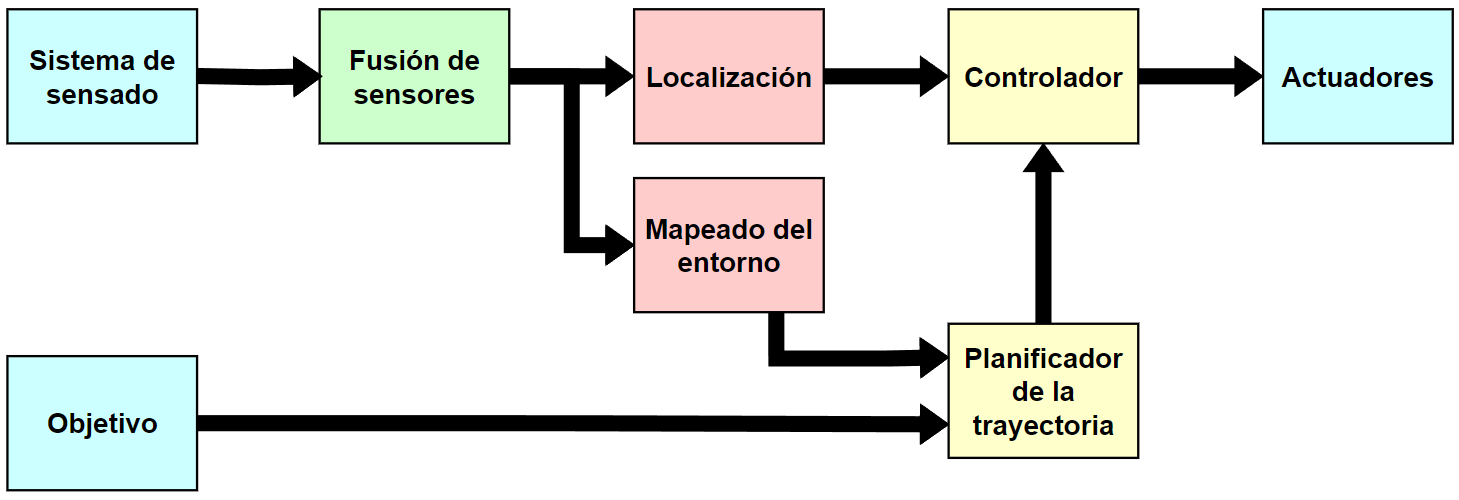
\includegraphics[scale=0.35]{images/control_theory_autnav.png}}
    \end{figure}


    \subsection{Planificadores globales y controladores}
    En las arquitecturas de navegación autónoma se distingue habitualmente entre \textit{planificación} y \textit{control}, dado que ambos
    procesos operan en escalas temporales distintas y persiguen objetivos complementarios. La planificación se encarga de generar una solución
    factible que conecte un estado inicial con un objetivo, imponiendo restricciones geométricas y de seguridad. Y por otro lado, el control
    ejecuta dicha solución en el sistema físico, transformando referencias en comandos actuables y compensando perturbaciones y la presencia de obstáculos.

    \subsubsection*{Planificadores}
    Los planificadores proporcionan una solución que permite que un vehículo navegue de forma segura en el espacio, dada una \textit{pose}
    inicial, un objetivo y un conjunto de restricciones (radio máximo de giro, modelo de movimiento, penalizaciones por cambios de trayectoria,
    heurística, entre otras). En función de los requisitos de la aplicación existen múltiples algoritmos y variantes, cada uno con ventajas y
    limitaciones. El tiempo de cálculo suele ser elevado, por lo que, en general, se ejecutan de manera previa al movimiento del robot o a una
    frecuencia reducida.

    Entre los métodos clásicos destaca el algoritmo de \textit{Dijkstra}, basado en grafos, que explora de forma exhaustiva y garantiza el
    camino de coste mínimo a cambio de un coste computacional elevado en espacios discretizados de gran tamaño. El algoritmo \textit{A*} puede
    entenderse como una extensión de Dijkstra que introduce una heurística para guiar la búsqueda, manteniendo la optimalidad bajo condiciones
    adecuadas y reduciendo el tiempo de cálculo en la práctica. Por su parte, variantes como \textit{D*} (y \textit{D* Lite}) están diseñadas
    para replanificar de forma eficiente ante cambios en el mapa, mientras que métodos como \textit{SMA*} limitan el consumo de memoria a costa
    de posibles reexpansiones. Finalmente, en espacios continuos o de alta dimensionalidad son frecuentes los planificadores basados en muestreo,
    como \textit{RRT} y \textit{RRT*}, mientras que algoritmos como \textit{DWA} se emplean habitualmente como planificadores locales al generar
    comandos de velocidad en tiempo real.

    En la Tabla~\ref{tab:planners_summary} se recogen, de forma comparativa, algunas ventajas y desventajas de los métodos más utilizados.

    \begin{table}[H]
        % \centering
        
        % \ttabbox
        {\caption{Tabla comparativa de planificadores para la navegación autónoma}
        \label{tab:planners_summary}}
        {%
        \begin{tabularx}{0.896\textwidth}{|c|c|c|}
            \hline
            \textbf{Método} & \textbf{Ventajas} & \textbf{Desventajas} \\
            \hline
            Dijkstra & Coste mínimo. & Alto coste computacional. \\
            \hline
            A* & Más eficiente que Dijkstra. & Dependencia de la heurística. \\
            \hline
            D* & Replanificación eficiente. & Mayor complejidad. \\
            \hline
            RRT & Eficiente en alta dimensionalidad. & Trayectoria subóptima. \\
            \hline
            RRT* & Converge asintóticamente. & Mayor tiempo de cómputo. \\
            \hline
            DWA & Respeta restricciones cinemáticas. & Propenso a mínimos locales. \\
            \hline
            SMA* & A* con memoria acotada. & Puede reexpandir nodos. \\
            \hline
            \multicolumn{3}{l}{Fuente: elaboración propia.} \\
        \end{tabularx}%
        }
    \end{table}

    En la práctica, una arquitectura robusta combina un planificador global con un planificador local: el primero define una ruta de alto
    nivel y el segundo adapta el movimiento a las condiciones reales del entorno (obstáculos no mapeados o dinámicos), respetando las
    restricciones de seguridad y la dinámica del vehículo. A este componente local se le suele denominar \textit{controlador} o, en algunos
    enfoques, planificador local.

    \subsubsection*{Planificador local}
    El planificador local transforma la referencia (trayectoria, posición o velocidad deseada) en comandos para el sistema de propulsión y los
    actuadores. En robótica móvil se emplean controladores clásicos como PID o LQR, así como métodos específicos para el seguimiento de
    trayectorias y la evitación local, tales como \textit{Pure Pursuit},Figura~\ref{fig:purepursuit}, o los \textit{campos potenciales}. Asimismo, el control predictivo
    basado en modelo (MPC) permite incorporar restricciones explícitas y anticipar la evolución del sistema, a costa de un mayor coste de
    cómputo. De forma general, se emplean lazos internos a alta frecuencia para estabilizar la actitud y la dinámica rápida, y lazos externos a
    menor frecuencia para regular la posición y ejecutar la navegación.

    En la Tabla~\ref{tab:controllers_summary} se resumen ventajas y desventajas de algunos controladores ampliamente utilizados.

    \begin{table}[H]
        \ttabbox
        {\caption{Tabla comparativa de controladores para la navegación autónoma}
        \label{tab:controllers_summary}}
        {%
        \begin{tabularx}{0.942\textwidth}{|c|c|c|}
            \hline
            \textbf{Método} & \textbf{Ventajas} & \textbf{Desventajas} \\
            \hline
            PID & Implementación simple y robusta. & Sin restricciones explícitas. \\
            \hline
            LQR & Estabilidad y rendimiento. & Requiere un modelo linealizado. \\
            \hline
            MPC & Anticipa la evolución del sistema. & Dependencia del modelo. \\
            \hline
            PP & Seguimiento sencillo (\textit{look-ahead}). & Propenso a oscilar. \\
            \hline
            APF & Reacción local rápida. & Propenso a mínimos locales. \\
            \hline
            \multicolumn{3}{l}{Fuente: elaboración propia.} \\
        \end{tabularx}%
        }
    \end{table}

La selección de planificador y controlador depende del entorno, del nivel de incertidumbre y, especialmente, de las
restricciones computacionales y temporales del sistema objetivo.

\begin{figure}[H]
    \ffigbox[\FBwidth] {
        \caption[Ejemplo de control por Pure Pursuit]{Ejemplo de control mediante Pure Pursuit.}
        \label{fig:purepursuit}
    }
    {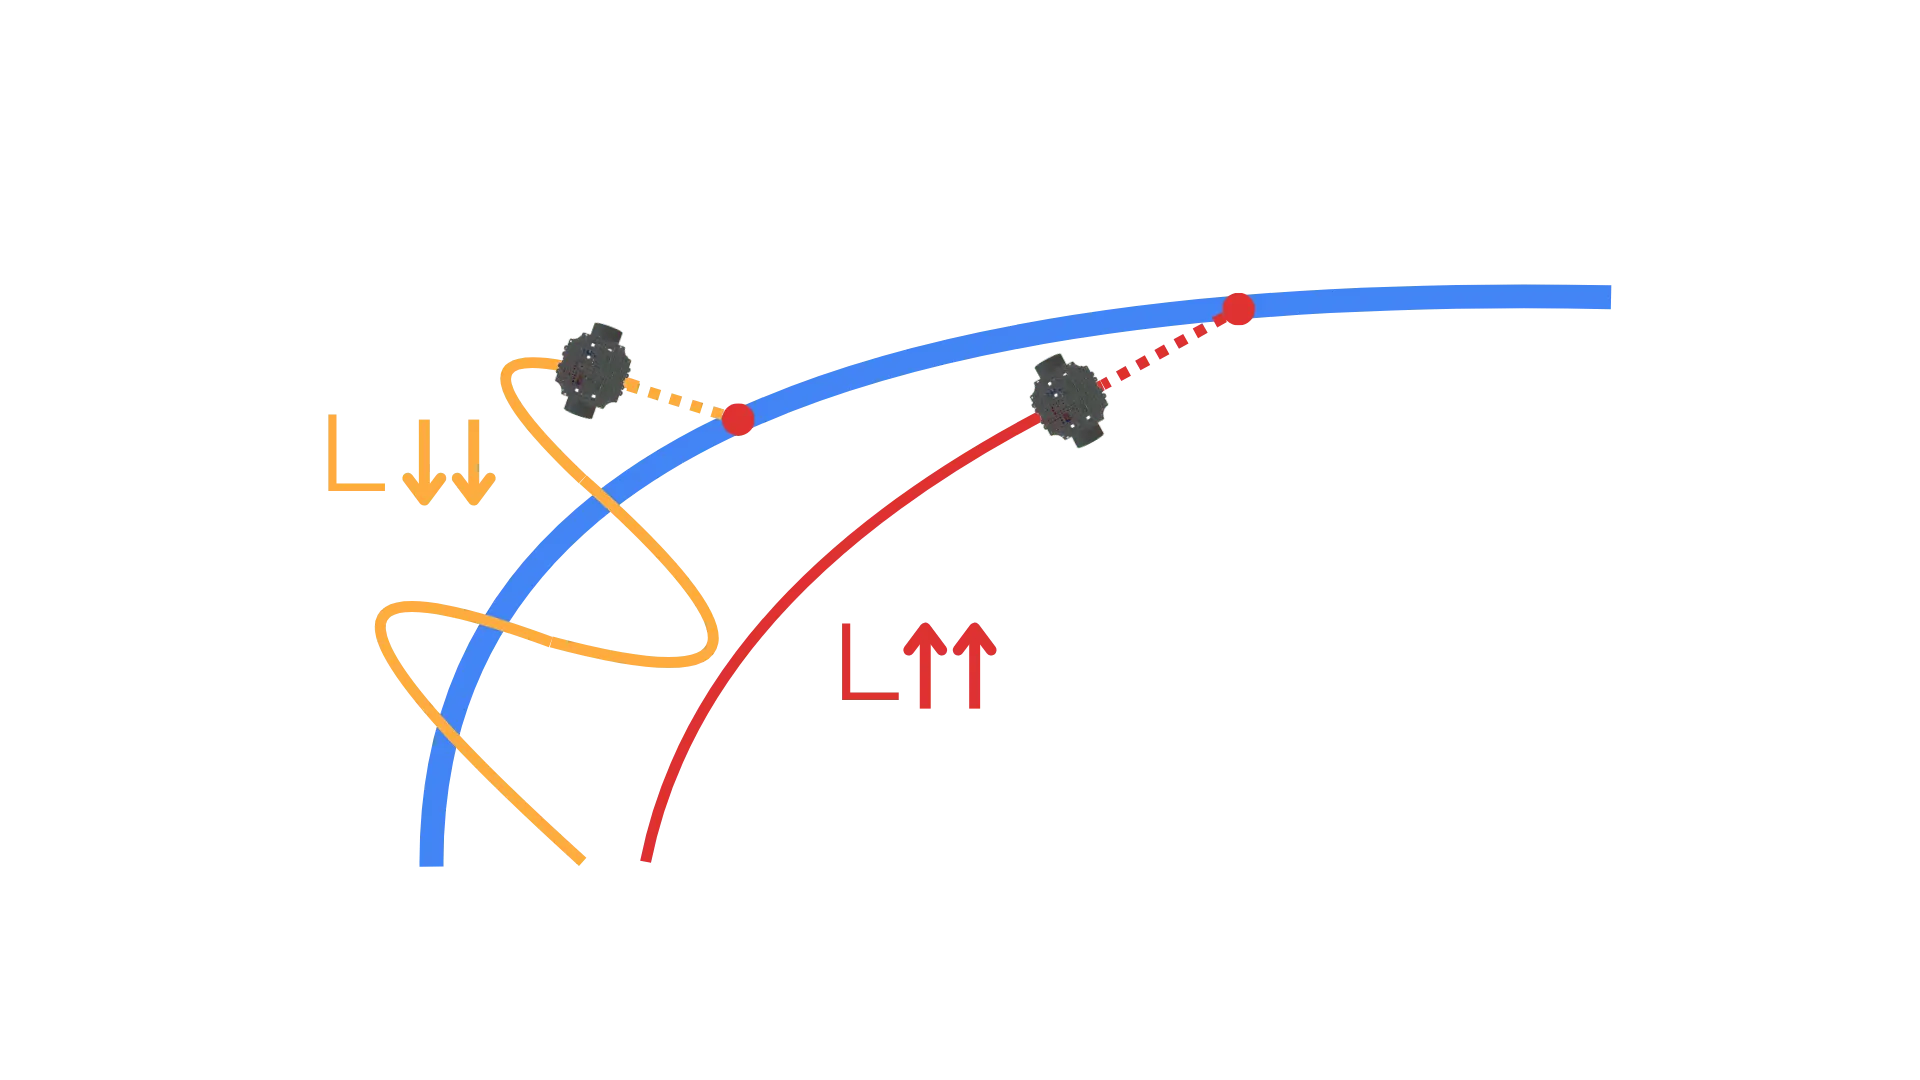
\includegraphics[scale=0.18]{images/pute_purpursuit.png}}
\end{figure}

    \subsection{Control mediante fusión visual-inercial(VI)}
    En el control aplicado a la navegación es habitual distinguir dos fuentes de estimación del estado con características complementarias. En
    primer lugar, se dispone de una fuente \textit{global} que proporciona una localización absoluta con alta precisión y sin deriva temporal,
    aunque normalmente a baja frecuencia (típicamente entre 1 y 10~Hz). En segundo lugar, se emplea una fuente \textit{local} u odométrica que,
    si bien acumula deriva con el tiempo, aporta estimaciones de manera continua a mayor frecuencia (del orden de 10 a 100~Hz), permitiendo
    mantener información del estado entre actualizaciones del sensor global. En la Figura~\ref{fig:loca-glob-loc} se ilustra este esquema: el
    localizador global corrige periódicamente la posición, mientras que, entre correcciones, la odometría estima el movimiento con un error que
    tiende a crecer con el tiempo. Mediante la fusión de ambas fuentes es posible obtener una estimación que combina localización absoluta sin
    deriva con disponibilidad continua a alta frecuencia.


    Generalmente, esta arquitectura se implementa mediante el uso de GNSS/GPS en exteriores o mediante Lidar y/o camaras 3D en itneriores como fuente global y el uso de
    encoders o IMUs como fuente odométrica. Estas son combinadas de manera estadisticas con un filtro, como puede ser un filtro de Kalma. En el caso de interés de este 
    trabajo, el localizador global suele basarse en información visual, mediante la extracción de
    características de una imagen 2D junto con la medida de una IMU a alta frecuencia para así, mantener una estimación continua del estado.
    \begin{figure}[H]
        \ffigbox[\FBwidth]{
            \caption[Esquema teórico de localización mediante odometría y sensor global]{Esquema teórico de localización mediante odometría y sensor global.}
            \label{fig:loca-glob-loc}
        }{
            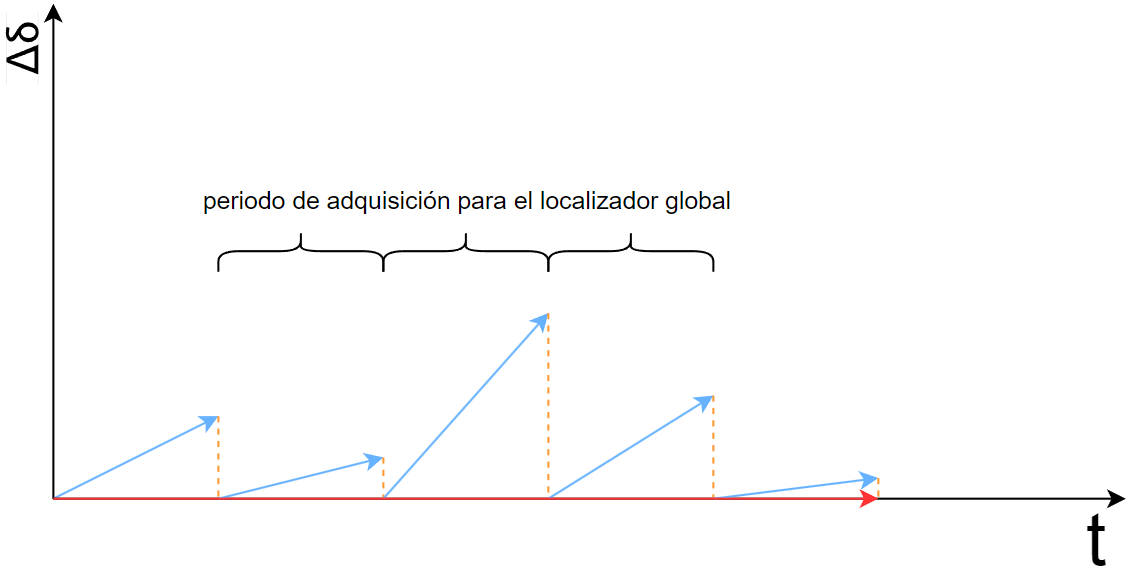
\includegraphics[scale=0.4]{images/localizador-global-local.png}
        }
    \end{figure}

    Desde la perspectiva del control, los sistemas VI se integran típicamente en una arquitectura jerárquica. En los lazos internos, el
    autopiloto estabiliza la actitud y regula la velocidad angular utilizando directamente la IMU, que ofrece tasas de actualización elevadas.
    En los lazos externos, la estimación de posición y velocidad proporcionada por VIO/VI-SLAM se emplea para generar referencias de movimiento
    (velocidades lineales, aceleraciones deseadas o puntos de paso) que guían el desplazamiento. Dado que la estimación visual puede estar
    limitada por la tasa de fotogramas, las condiciones de iluminación o la ausencia de textura, es habitual emplear fusión temporal para
    aprovechar simultáneamente la alta frecuencia de la IMU y la capacidad correctiva de la cámara.

    Un aspecto relevante en la navegación VI es la gestión de incertidumbre y latencia. La estimación visual suele introducir retardo de
    procesamiento. En consecuencia, el diseño del controlador debe considerar dichas latencias para evitar inestabilidades, por ejemplo mediante predicción del
    estado al tiempo actual, filtrado de medidas o reducción de la agresividad de maniobra cuando disminuye la confianza en la estimación. De
    forma análoga, el sistema debe contemplar condiciones adversas como cambios bruscos de iluminación, desenfoque por movimiento u oclusiones que pueden degradar la 
    calidad de la odometría. En tales casos, la IMU actúa como soporte.

    En aplicaciones prácticas, el enfoque VI condiciona también decisiones de diseño a nivel de percepción. La elección de cámara (\textit{global
    shutter} frente a \textit{rolling shutter}), la calibración intrínseca y extrínseca, la sincronización temporal entre cámara e IMU y el
    modelado adecuado de sesgos inerciales influyen de forma directa en la estabilidad del control. En particular, la sincronización resulta
    crítica: errores temporales pequeños pueden traducirse en estimaciones inconsistentes. Por ello, los
    sistemas VI robustos priorizan una cadena de adquisición bien caracterizada y procedimientos de calibración robustos.


    % \subsection{Mención honorífica, ROS}
    % ROS (\textit{Robot Operating System}) ha desempeñado un papel fundamental en la consolidación de arquitecturas modulares en robótica,
    % facilitando la reutilización de algoritmos y acelerando la integración de sistemas complejos. Su modelo basado en \textit{nodos} que
    % intercambian información mediante \textit{tópicos}, \textit{servicios} y \textit{acciones} permite desacoplar componentes de percepción,
    % localización, planificación y control. Esta separación favorece la mantenibilidad y permite sustituir módulos sin modificar el resto del
    % sistema, siempre que se conserven las interfaces, lo cual resulta especialmente valioso en proyectos de investigación y desarrollo donde
    % la iteración es constante.

    % Dentro de este ecosistema, Nav2 (Navigation2) representa una arquitectura versátil para navegación en ROS~2, diseñada para integrarse de
    % manera flexible con diferentes sensores, fuentes de localización y estrategias de planificación y control. Su estructura se apoya en un
    % conjunto de servidores especializados (\textit{planner server}, \textit{controller server}, \textit{behavior server}, entre otros),
    % conectados mediante \textit{actions} y gobernados por \textit{behavior trees}, lo que permite definir comportamientos complejos de forma
    % declarativa. Esta arquitectura facilita sustituir planificadores y controladores mediante plugins, ajustar parámetros sin alterar código y
    % adaptar el sistema a distintos requisitos de hardware o de entorno.

    % En consecuencia, ROS y, en particular, Nav2, han contribuido de forma notable a que la implementación de arquitecturas de navegación sea
    % más accesible y reproducible. La modularidad inherente reduce el esfuerzo de integración y permite centrar el desarrollo en componentes
    % específicos (por ejemplo, percepción o estimación de profundidad), manteniendo una infraestructura estable para la coordinación del sistema.
    \section{Localización (VIO)}
    La localización constituye uno de los bloques fundamentales en un sistema de navegación autónoma, ya que permite estimar la \textit{pose}
    del vehículo a partir de la información sensorial disponible. En el caso de plataformas aéreas, esta estimación debe
    obtenerse con baja latencia, suficiente precisión y un coste computacional compatible con las restricciones del sistema.

    En este contexto, la odometría visual-inercial (\textit{Visual-Inertial Odometry}, VIO) permite estimar el movimiento relativo del sensor
    combinando imágenes de una o varias cámaras con medidas proporcionadas por una unidad de medida inercial (IMU). A diferencia de un sistema
    SLAM completo, cuyo objetivo incluye la construcción y mantenimiento de un mapa global del entorno, un sistema VIO se centra principalmente
    en estimar de forma local y continua la trayectoria del vehículo respecto a un marco de referencia inicial. Por tanto, la salida principal
    del sistema es una estimación de posición, orientación y, en muchos casos, velocidad.

    Desde un punto de vista funcional, un sistema VIO suele estar formado por dos bloques principales. El primero es un \textit{front-end}
    visual, encargado de procesar las imágenes, detectar o seguir características y generar correspondencias temporales entre fotogramas. El
    segundo es un estimador de estado, que combina dichas observaciones visuales con las medidas de la IMU mediante técnicas de filtrado u
    optimización. La IMU permite propagar el estado a alta frecuencia entre imágenes consecutivas, mientras que la información visual corrige la
    deriva acumulada por la integración inercial.

    A nivel estructural, los sistemas VIO suelen organizarse en etapas de inicialización, propagación inercial, seguimiento visual y actualización
    del estado. La inicialización permite estimar condiciones iniciales como la dirección de la gravedad, los sesgos de la IMU y la primera
    referencia local del sistema. Posteriormente, las medidas inerciales se integran entre fotogramas consecutivos para predecir la evolución de
    la orientación, la velocidad y la posición. Finalmente, las observaciones visuales se emplean para corregir esta predicción, reduciendo la
    deriva y mejorando la consistencia de la estimación.

    Existen dos familias principales de métodos VIO: los enfoques basados en filtrado y los enfoques basados en optimización. Los primeros, como
    los basados en filtros de Kalman extendidos, actualizan el estado de forma recursiva a medida que llegan nuevas medidas. Los segundos formulan
    el problema como una optimización sobre una ventana temporal de estados, incorporando restricciones visuales e inerciales de forma conjunta.
    En ambos casos, es habitual estimar no solo posición y orientación, sino también velocidad, sesgos del acelerómetro y del giróscopo.

    Una diferencia importante entre VIO y VI-SLAM es el alcance de la estimación. Mientras que VI-SLAM incorpora mecanismos de mapeado,
    relocalización y cierre de bucle para mantener una representación global consistente del entorno, VIO se centra en la estimación local del
    movimiento. Por este motivo, la VIO puede acumular deriva a largo plazo, pero suele presentar menor complejidad computacional y menor latencia,
    lo que la hace especialmente atractiva para aplicaciones de control en tiempo real.

    La literatura reciente recoge múltiples sistemas representativos dentro de la odometría visual-inercial, con diseños que priorizan distintos
    compromisos entre precisión, robustez y coste computacional. Por ejemplo, se han propuesto métodos basados en filtrado, como RVIO, y métodos
    basados en optimización sobre ventanas deslizantes, como VINS-Mono. También existen sistemas más completos, como ORB-SLAM3, que pueden operar
    en modo visual-inercial e incorporar capacidades propias de SLAM, aunque con una complejidad superior. Estos enfoques muestran que la elección
    de la arquitectura depende directamente de los requisitos de la aplicación, especialmente de la frecuencia de actualización, la disponibilidad
    de cómputo y la necesidad, o no, de consistencia global a largo plazo \cite{overview-vslam}.
    
    En este trabajo, la localización se plantea como un problema de odometría visual-inercial robocéntrica. El sistema estima la evolución del
    UAV respecto al instante inicial de navegación, utilizando la IMU para propagar el estado y las observaciones visuales para corregir dicha
    propagación. Esta formulación resulta adecuada para el objetivo del proyecto, ya que no se requiere construir un mapa global persistente del
    entorno, sino disponer de una estimación local suficientemente precisa y estable para alimentar los módulos de planificación, control y
    evitación de obstáculos.
    
\section{Estimadores de profundidad}

    La estimación de profundidad a partir de visión monocular (\textit{Monocular Depth Estimation}, MDE) persigue recuperar, para cada 
    píxel de una imagen, una medida de distancia respecto a la cámara. En términos generales, los enfoques modernos formulan el problema 
    como una tarea de predicción densa en la que una red neuronal extrae características visuales globales y locales y, posteriormente, un 
    decodificador reconstruye un mapa de profundidad con resolución similar a la entrada. En arquitecturas actuales basadas en 
    \textit{Transformers} de visión, el proceso se divide habitualmente en un \textit{backbone} (codificador) que transforma la imagen en 
    un conjunto de \textit{tokens} y un \textit{head} de predicción que reensambla y fusiona dichas características para producir una salida 
    densa. Un ejemplo representativo de este paradigma es el uso de un \textit{Vision Transformer} preentrenado como extractor de 
    características y un decodificador tipo DPT (\textit{Dense Prediction Transformer}) como cabeza de salida, estrategia que se emplea en 
    los modelos recientes de la familia Depth Anything.

    Además de la profundidad monocular clásica, la tendencia reciente ha ampliado el objetivo hacia la recuperación de geometría consistente 
    a partir de múltiples vistas, incorporando de forma explícita información de cámara (poses) cuando se dispone de ella o estimándola 
    cuando no es conocida. 

    \subsection{Modelos recientes para la inferencia de profundidad}
    En el marco de modelos generalistas para estimación de profundidad, MiDaS se ha consolidado como una referencia práctica debido a su 
    buena capacidad de generalización y a su disponibilidad en múltiples variantes. Su estrategia de entrenamiento combina datos de 
    distintos dominios y pérdidas diseñadas para favorecer la coherencia relativa, lo que suele traducirse en estimaciones robustas en 
    escenarios variados.

    Por su parte, la serie Depth Anything representa una evolución hacia modelos fundacionales de geometría visual. En el caso de 
    Depth Anything 3, el objetivo explícito se extiende a la reconstrucción del espacio visual a partir de cualquier número de vistas, 
    con o sin poses de cámara conocidas. El modelo se apoya en dos principios de diseño: (i) un único \textit{transformer} preentrenado es 
    suficiente como \textit{backbone} sin necesidad de arquitecturas especializadas, y (ii) un conjunto mínimo de objetivos de predicción 
    (profundidad y rayos) puede reemplazar estrategias multitarea más complejas.

    A nivel arquitectónico, Depth Anything 3~\cite{overview-da} utiliza un \textit{Vision Transformer} preentrenado (p.\,ej., DINOv2) y habilita el 
    razonamiento entre vistas mediante un mecanismo de autoatención adaptativo que reorganiza los \textit{tokens} para alternar atención 
    intra-vista y entre-vistas. Sobre las características del \textit{backbone}, el modelo incorpora un \textit{Dual-DPT head} que produce 
    simultáneamente un mapa de profundidad y un mapa de rayos, compartiendo módulos de reensamblado y diferenciándose en la etapa de fusión 
    final. Adicionalmente, cuando se dispone de parámetros de cámara, estos pueden incorporarse mediante un codificador ligero que genera 
    \textit{camera tokens} y los concatena con los \textit{patch tokens}, participando en las operaciones de atención.

    La profundidad real en conjuntos capturados con sensores suele ser incompleta o ruidosa. Para mitigar este problema, se entrena un 
    modelo que sirve como maestro o profesor generando pseudo-etiquetas densas de alta calidad que posteriormente 
    se alinean con medidas métricas ruidosas o dispersas mediante un ajuste robusto de escala y desplazamiento (p.\,ej., RANSAC). 
    Esta estrategia incrementa el detalle y la completitud de las etiquetas manteniendo la coherencia geométrica necesaria para tareas 
    posteriores~\cite{overview-da}.

    \subsection{Limitaciones físicas y computacionales}
    A pesar de los avances, los estimadores monoculares de profundidad presentan limitaciones inherentes. La más relevante, en escenarios 
    generales, es que la predicción suele ser \textit{relativa}: sin información adicional (calibración, escala conocida o múltiples vistas), 
    la profundidad monocular no determina de forma única la escala métrica, lo que obliga a realizar alineamientos posteriores 
    (escala y/o desplazamiento) cuando se requiere una medida absoluta. En Depth Anything 3 esta problemática se aborda explícitamente 
    mediante alineamiento de pseudo-profundidad con medidas métricas disponibles y, en el caso multivista~\cite{overview-da}, mediante el uso combinado de 
    mapas de profundidad y rayos para recuperar geometría consistente.

    Asimismo, estos modelos están sujetos a errores sistemáticos que dependen del dominio: cambios de iluminación, superficies reflectantes 
    o translúcidas, regiones con baja textura y oclusiones pueden degradar la estimación. El documento señala de forma directa que parte de 
    los datos reales presentan deficiencias severas (profundidades incompletas o ruidosas), lo que motiva el uso de pseudo-etiquetado y 
    procedimientos de filtrado y preprocesado para descartar muestras problemáticas (p.\,ej., desalineamientos imagen--profundidad, recortes 
    o valores erróneos). Este hecho pone de manifiesto que, incluso con modelos generalistas, la calidad de los datos y la coherencia de 
    supervisión condicionan el comportamiento final del estimador.

    Desde el punto de vista computacional, los modelos de última generación basados en \textit{Transformers} implican un coste elevado tanto 
    en entrenamiento como en inferencia. Depth Anything 3 reporta entrenamiento a gran escala y evalúa variantes con distinto número de 
    parámetros, mostrando que el rendimiento mejora con el escalado del modelo y de los datos, pero a costa de mayores requisitos de 
    hardware. Además, la extensión a múltiples vistas incrementa el coste por el crecimiento del número de \textit{tokens} y por los 
    mecanismos de atención entre vistas. En~\cite{overview-da} se cuantifican velocidades de ejecución y se discuten límites prácticos en el número 
    máximo de imágenes procesables en GPU en el caso de Depth Anything 3, lo que evidencia que, aunque existan variantes 
    compactas, la carga computacional continúa siendo un factor determinante para su despliegue en sistemas con recursos limitados.

    Por último, en aplicaciones robóticas la latencia y la estabilidad temporal son críticas. Incluso cuando la inferencia se realiza a 
    resolución reducida, la estimación puede introducir retardos que afectan a la frecuencia efectiva del lazo de control. En consecuencia, 
    resulta habitual adoptar compromisos entre resolución, complejidad del modelo y tasa de actualización, o bien trasladar el cómputo a 
    hardware más capaz (p.\,ej., GPU dedicada) para cumplir restricciones de tiempo real. En este trabajo, estas limitaciones motivan la 
    selección cuidadosa de modelos y su optimización, así como el uso de métricas orientadas no solo a la precisión, sino también a la 
    estabilidad y al coste computacional de la inferencia.
\chapter{Arquitectura del sistema}

El sistema se ha dividido en dos módulos: la plataforma aérea y la estación de tierra. La plataforma aérea está compuesta 
por el propio UAV y una Jetson Nano, que actúa como pasarela de comunicación entre el UAV y la estación de tierra.

Esta pasarela adquiere la información visual e inercial procedente de la cámara a bordo, una Intel RealSense D435i, y la separa 
en tres canales. El canal de profundidad se almacena en una tarjeta SD para su posterior comparación y validación con el algoritmo 
de navegación. El canal visual se reenvía mediante un flujo RTSP a través de Wi-Fi hasta la estación de tierra, con el objetivo de 
minimizar la latencia y maximizar el rendimiento. Finalmente, el canal inercial, correspondiente a la IMU, se envía mediante un 
socket UDP hasta la estación de tierra. De esta forma, se gestionan adecuadamente las distintas frecuencias de muestreo empleadas 
por cada uno de los sensores.

En la Figura \ref{fig:plataforma_aerea} se muestra la arquitectura general de la plataforma aérea.

\begin{figure}[H]
    \ffigbox[\FBwidth] {
        \caption[Arquitectura de la plataforma aérea]{Arquitectura de la plataforma aérea.}
        \label{fig:plataforma_aerea}
    }
    {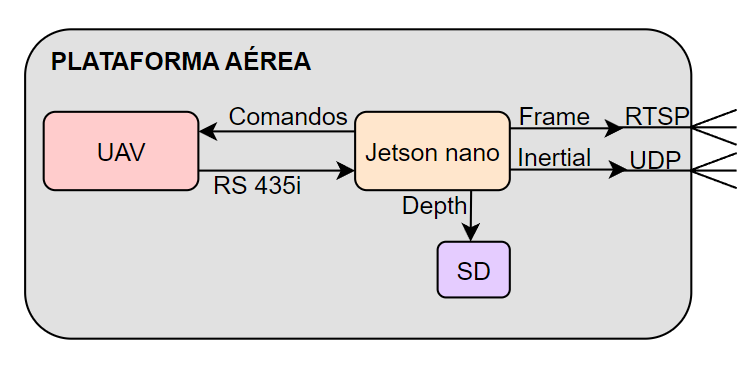
\includegraphics[scale=0.7]{images/plataforma_aerea.png}}
\end{figure}

En la estación de tierra se ejecuta el algoritmo de navegación, aprovechando la capacidad de cómputo de un ordenador central más 
potente que el sistema embarcado. Esta estación recibe la información visual e inercial procedente de la plataforma aérea y la 
adapta para ser utilizada como entrada del algoritmo de navegación. Además, el sistema recibe como entrada un conjunto de 
\textit{waypoints} definidos por el usuario.

En primer lugar, los canales visual e inercial se procesan mediante un sistema de odometría visual-inercial, encargado de estimar 
la pose del UAV respecto al punto de inicio del algoritmo. De forma paralela, el canal visual se introduce en un estimador de 
profundidad que, junto con un algoritmo de evitación de obstáculos, proporciona una dirección de movimiento segura.

Toda esta información, junto con la trayectoria generada por el planificador global, se introduce en un planificador local. Este 
genera las referencias necesarias para un controlador PID, encargado de obtener el control en velocidad del dron. Finalmente, el 
comando de velocidad, compuesto por sus componentes lineal y angular, se envía mediante UDP de vuelta al dron para su ejecución.

En la Figura \ref{fig:estacion_tierra} se muestra la arquitectura general de la estación de tierra.


\begin{figure}[H]
    \ffigbox[\FBwidth] {
        \caption[Arquitectura de la estación de tierra]{Arquitectura de la estación de tierra.}
        \label{fig:estacion_tierra}
    }
    {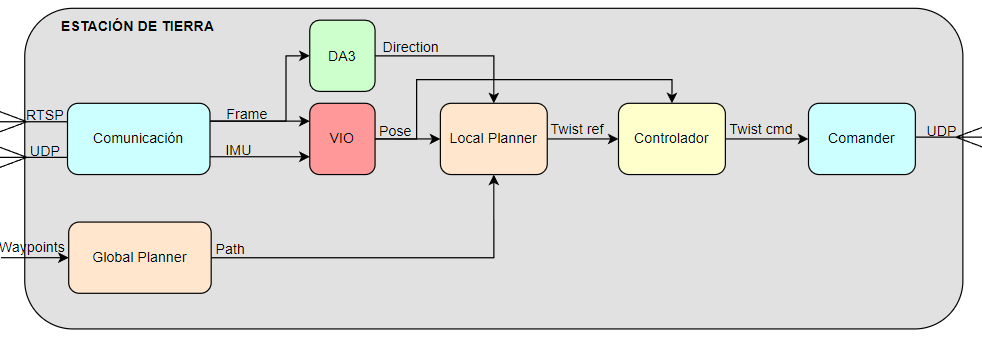
\includegraphics[scale=0.55]{images/estacion_tierra.png}}
\end{figure}

\section{Descripción de componentes del sistema}

La plataforma aérea cuenta con un controlador de vuelo Orange Cube, mostrado en la Figura~\ref{fig:orange_cube}. Este dispositivo 
se encarga del control de bajo nivel del UAV y permite comandar la plataforma mediante consignas de velocidad y actitud. Sus 
características principales son:

\begin{figure}[H]
    \ffigbox[\FBwidth] {
        \caption[Controlador Orange Cube]{Controlador Orange Cube.}
        \label{fig:orange_cube}
    }
    {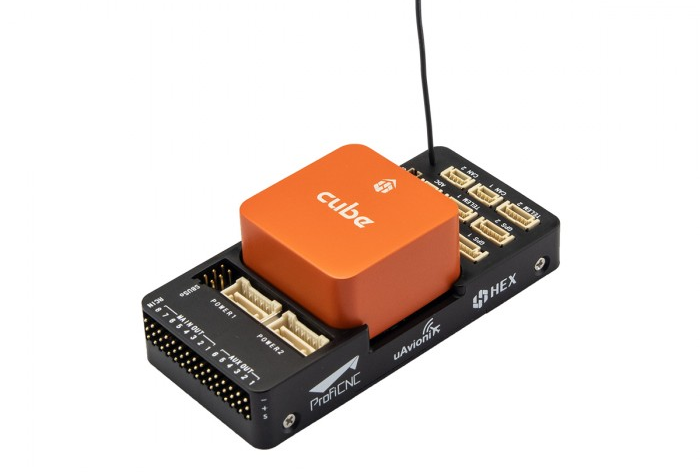
\includegraphics[scale=0.45]{images/orange_cube.png}}
\end{figure}

\begin{itemize}[nosep]
    \item Procesador STM32H753 Cortex\textsuperscript{\textregistered}-M7 con 1 MB de RAM y 2 MB de Flash.
    \item 1 IMU InvenSense ICM20602 y 1 IMU ICM20948.
    \item 2 barómetros MS5611.
    \item 1 magnetómetro AK09916.
    \item 1 acelerómetro y giroscopio ICM20649.
    \item Varios sensores de temperatura y conexión para GPS.
    \item 2 conectores para recepción de telemetría mediante protocolo UART.
\end{itemize}

En este proyecto, los sensores internos del controlador de vuelo no se emplean como fuente principal de percepción para el 
algoritmo de navegación desarrollado. Su uso queda asociado principalmente al control y estabilización de bajo nivel del UAV. El 
objetivo del sistema es lograr una navegación autónoma y una evitación de obstáculos estable a partir de la información visual e 
inercial proporcionada por la cámara embarcada.

Para ello, la plataforma aérea incorpora una cámara Intel RealSense D435i, mostrada en la Figura \ref{fig:rs_435i}, una cámara RGB-D basada en visión estéreo que integra 
una unidad de medida inercial. Este sensor permite obtener simultáneamente imágenes RGB, información de profundidad y medidas 
inerciales, lo que resulta especialmente adecuado para tareas de odometría visual-inercial, percepción tridimensional del entorno 
y evitación de obstáculos.

Las principales características de la Intel RealSense D435i son:


\begin{figure}[H]
    \ffigbox[\FBwidth] {
        \caption[Cámara RealSense 435i]{Cámara RealSense 435i.}
        \label{fig:rs_435i}
    }
    {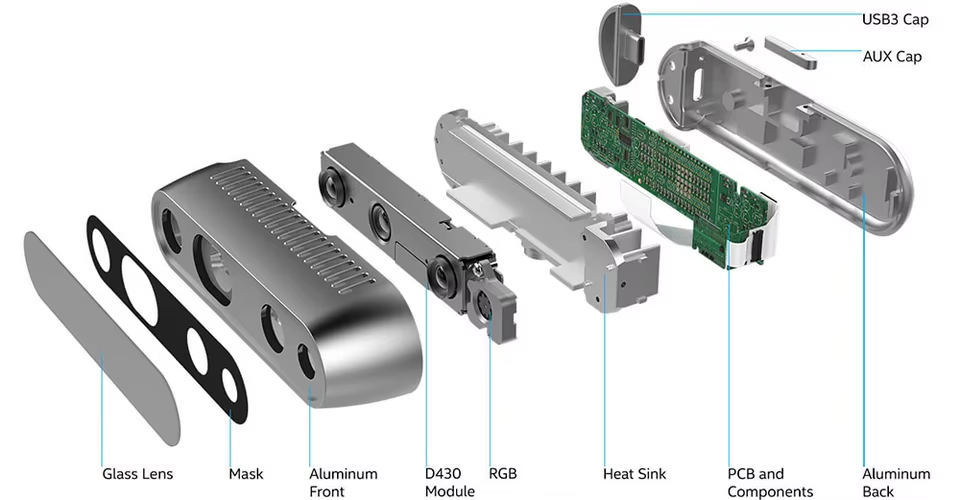
\includegraphics[scale=0.35]{images/rs_435i.png}}
\end{figure}


\begin{itemize}[nosep]
    \item Resolución de profundidad de hasta $1280 \times 720$ píxeles.
    \item Rango ideal de operación entre $0.3~\mathrm{m}$ y $3~\mathrm{m}$.
    \item Cámara RGB de $2~\mathrm{MP}$ con resolución de hasta $1920 \times 1080$ píxeles a $30~\mathrm{fps}$.
    \item Campo de visión del canal RGB de $69^\circ \times 42^\circ$.
    \item IMU Bosch BMI055 de 6 ejes, compuesta por acelerómetro a 200 Hz y un giroscopio a 100 Hz.
    \item Sincronización temporal de las muestras inerciales con los datos de profundidad mediante marcas de tiempo proporcionadas por el hardware.
    \item Conexión mediante USB-C 3.1 Gen 1.
    \item Dimensiones aproximadas de $90~\mathrm{mm} \times 25~\mathrm{mm} \times 25~\mathrm{mm}$.
\end{itemize}

La estación de tierra consta de un ordenador HP Probook, con un procesador intel core ULTRA 7, 32 GB de RAM y una gráfica 
NVIDIA GeForce RTX 2050 donde se ejecuta el programa de navegación autónoma.


\section{Resumen de algoritmia utilizada}

En esta sección se presenta una visión general de los principales módulos algorítmicos empleados en el sistema de navegación 
autónoma. El objetivo es describir de forma resumida el flujo completo de procesamiento, desde la recepción de los datos 
sensoriales hasta el envío de comandos de velocidad al UAV. Cada uno de estos bloques se desarrollará con mayor detalle en los 
apartados posteriores.

La recepción del canal visual se realiza mediante un flujo RTSP, lo que permite transmitir vídeo en tiempo real desde la 
plataforma aérea hasta la estación de tierra a través de Wi-Fi. Esta solución se ha seleccionado por su baja latencia, su 
compatibilidad con herramientas estándar de procesamiento de vídeo y su capacidad para mantener un flujo continuo de imágenes 
sin necesidad de almacenar todos los datos en memoria.

A partir de la información visual e inercial recibida, se implementa un sistema de odometría visual-inercial, basado 
conceptualmente en el enfoque propuesto en RVIO2~\cite{huai2022square} y ~\cite{huai2024consistent}. Este módulo estima la pose relativa del UAV respecto al instante 
inicial mediante la combinación de imágenes y medidas de la IMU. Aunque la arquitectura y algunos fundamentos teóricos se inspiran 
en dicho trabajo, el código empleado en este proyecto ha sido desarrollado de forma propia y adaptado a las necesidades 
específicas del sistema.

De forma complementaria, el canal visual se procesa mediante Depth Anything 3~\cite{overview-da}, utilizado como estimador de profundidad 
monocular. La información de profundidad obtenida permite generar una representación aproximada del entorno, que posteriormente 
se emplea en el módulo de evitación de obstáculos.

El sistema de planificación se divide en dos niveles. En primer lugar, el planificador global implementa una estrategia básica de 
tipo \textit{go-to}, encargada de generar una trayectoria de referencia hacia los \textit{waypoints} definidos por el usuario. En 
segundo lugar, el planificador local utiliza una variante tridimensional del algoritmo \textit{Pure Pursuit}, basado en~\cite{pp3d}, que permite adaptar 
la dirección de avance del UAV en función de la trayectoria global y de la información local del entorno.

Finalmente, las referencias generadas por el planificador local se introducen en un controlador PID, encargado de calcular los 
comandos de velocidad lineal y angular necesarios para guiar el UAV. Estos comandos se envían posteriormente al controlador de 
vuelo mediante comunicación UDP, cerrando así el ciclo de navegación.
\chapter{Comunicaciones}
\section{Pasarela de abordo}

El programa implementa una pasarela de comunicación entre la cámara Intel RealSense D435i y la estación de tierra. Su función 
principal es separar la información capturada por la cámara en distintos canales de comunicación: vídeo RGB transmitido mediante RTSP, 
datos inerciales enviados por UDP y datos de profundidad almacenados en un archivo \texttt{.bag} para su posterior análisis y validación.

La ejecución se organiza en varias tareas concurrentes. El hilo principal inicializa la configuración del sistema, lanza los hilos 
auxiliares y mantiene activo el servidor RTSP mediante el bucle principal de GStreamer. De forma paralela, un hilo supervisa la conexión 
de la cámara, otro adquiere los datos de la RealSense y un tercer hilo se encarga del envío periódico de la información inercial mediante 
UDP.


El flujo de ejecución comienza con la lectura de la configuración del sistema, donde se definen parámetros como el puerto RTSP, el punto 
de montaje, la resolución de imagen, la frecuencia de captura y el modo de depuración. En modo normal, el sistema espera a detectar la 
cámara física antes de iniciar la adquisición. En modo depuración, los datos se leen directamente desde un archivo \texttt{.bag}, lo que 
permite reproducir capturas previas sin necesidad de disponer de la cámara conectada.

Una vez iniciada la adquisición, cada paquete recibido desde la RealSense se clasifica según su tipo de flujo. Las muestras del giroscopio 
y del acelerómetro se escalan y almacenan en la estructura compartida \texttt{rs\_data}. Las imágenes RGB se encapsulan en buffers de 
GStreamer y se introducen en el elemento \texttt{appsrc}, desde donde son codificadas en H.264 y publicadas mediante RTSP. Por otro lado, 
el canal de profundidad se almacena en el archivo de registro para su posterior comparación con los resultados obtenidos por el algoritmo 
de navegación.

La comunicación con la estación de tierra se habilita mediante un mecanismo de conexión por UDP. Cuando el cliente envía un mensaje de 
establecimiento de conexión, el sistema almacena su dirección y activa el envío periódico de datos inerciales. Esta misma variable de 
estado también se utiliza para controlar el envío del flujo de vídeo, evitando introducir imágenes en el servidor RTSP cuando no existe 
ningún cliente conectado.

La arquitectura de funcionamiento se muestra en la Figura~\ref{fig:threads_comms}

\begin{figure}[H]
    \ffigbox[\FBwidth] {
        \caption[Arquitectura de funcionamiento de la pasarela.]{Arquitectura de funcionamiento de la pasarela.}
        \label{fig:threads_comms}
    }
    {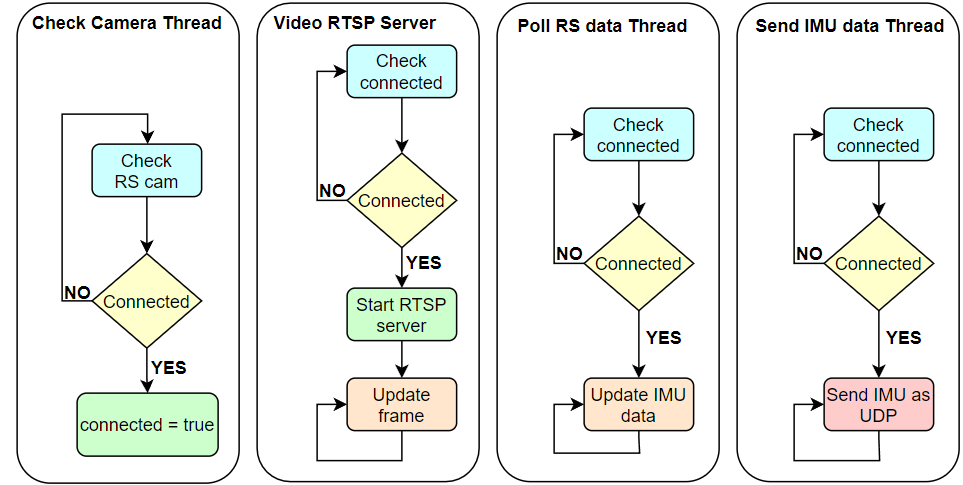
\includegraphics[scale=0.55]{images/threads_pasarela.png}}
\end{figure}


\section{Recepción de datos}

\subsection{Proceso de adquisición y sincronización de datos}

El módulo de adquisición se encarga de leer los datos procedentes de la Jetson Nano y generar paquetes de entrada 
sincronizados para el algoritmo de navegación. Cada paquete contiene una imagen RGB y un conjunto de muestras inerciales comprendidas 
entre dos imágenes consecutivas.

El proceso comienza en la incialización del receptor RTSP y la creación del socket UDP para la recepción de los 
datos inerciales.

Una vez inicializado el sistema, se lanza un hilo de adquisición. Este hilo se ejecuta interativamente. Las muestras 
inerciales se almacenan en un buffer independiente, uno para el acelerómetro y otro para el giróscopo. Cada muestra queda asociada a una 
marca temporal.

Cuando se recibe una imagen RGB válida, el algoritmo comprueba que existan suficientes muestras de IMU antes y después del instante de 
captura de la imagen. A continuación, se seleccionan los instantes de integración comprendidos entre la imagen anterior y la imagen actual. Para 
cada uno de estos instantes se interpolan las medidas del acelerómetro y del giróscopo, generando así una secuencia de muestras 
inerciales sincronizadas con el intervalo visual.


Finalmente, se construye un paquete, que contiene la imagen RGB y el conjunto de 
muestras IMU interpoladas. Este paquete se introduce en una cola de salida, desde donde puede ser 
consumido posteriormente por el algoritmo de navegación. Este proceso se muestra en la Figura~\ref{fig:frame_imu}.

\begin{figure}[H]
    \ffigbox[\FBwidth] {
        \caption[Esquema de adquisición de datos.]{Esquema de adquisición de datos.}
        \label{fig:frame_imu}
    }
    {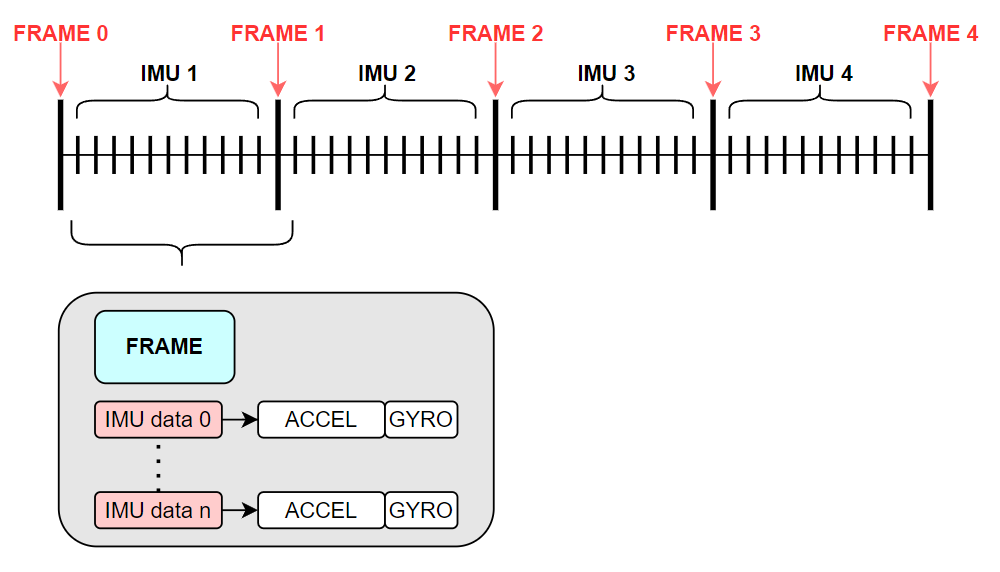
\includegraphics[scale=0.55]{images/frame_imu_arq.png}}
\end{figure}



\subsection{Interpolación de medidas inerciales}

Las medidas de la IMU se adquieren a frecuencias diferentes y no están necesariamente sincronizadas con los fotogramas 
visuales. Por ello, se realiza una interpolación lineal de las medidas inerciales, de forma que se obtenga una muestra de 
acelerómetro y giróscopo en los mismos instantes temporales. Además, se fuerza que la última muestra inercial del paquete 
coincida temporalmente con el fotograma visual correspondiente.

Sea un buffer de muestras inerciales definido como $\mathcal{B}$, donde cada muestra está formada por una marca 
temporal $t_i$ y una medida vectorial $\mathbf{v}_i \in \mathbb{R}^3$, correspondiente a una aceleración o a una velocidad 
angular:

\begin{equation}
\begin{aligned}
    \mathcal{B}&=\left\{\left(t_0, \mathbf{v}_0\right),\left(t_1, \mathbf{v}_1\right),\ldots,\left(t_N, \mathbf{v}_N\right)\right\},\\[2mm]\mathbf{v}_i&=
    \begin{bmatrix}
        v_{x,i} &
        v_{y,i} &
        v_{z,i}
    \end{bmatrix}^{T}.
\end{aligned}
\end{equation}

Para obtener el valor de la IMU en un instante $t$, el algoritmo busca dos muestras consecutivas que encierren dicho 
instante. Si $t$ queda fuera del intervalo temporal disponible, la interpolación se considera no válida:

\begin{equation}
\begin{aligned}
    t_i \leq t \leq t_{i+1},
    \qquad
    t \in \left[t_0,t_N\right].
\end{aligned}
\end{equation}

Una vez localizado el intervalo, se calcula el factor de interpolación lineal $\alpha$ y se obtiene la medida interpolada 
$\mathbf{v}(t)$ como combinación lineal entre las dos muestras consecutivas:

\begin{equation}
\begin{aligned}
    \Delta t_i
    &=
    t_{i+1}-t_i,
    \\[1mm]
    \alpha
    &=
    \frac{t-t_i}{\Delta t_i},
    \\[1mm]
    \mathbf{v}(t)
    &=
    \mathbf{v}_i
    +
    \alpha
    \left(
        \mathbf{v}_{i+1}
        -
        \mathbf{v}_i
    \right).
\end{aligned}
\label{eq:interpolacion_imu}
\end{equation}

De forma equivalente, la interpolación anterior puede expresarse por componentes como

\begin{equation}
    \mathbf{v}(t)
    =
    \begin{bmatrix}
        v_{x,i} + \alpha \left(v_{x,i+1} - v_{x,i}\right) \\
        v_{y,i} + \alpha \left(v_{y,i+1} - v_{y,i}\right) \\
        v_{z,i} + \alpha \left(v_{z,i+1} - v_{z,i}\right)
    \end{bmatrix}.
\end{equation}

En el caso particular en el que dos muestras consecutivas tengan prácticamente la misma marca temporal, se evita la 
división por un valor cercano a cero y se asigna directamente la primera muestra del intervalo:

\begin{equation}
    \mathbf{v}(t)
    =
    \begin{cases}
        \mathbf{v}_i
        &
        \text{si }
        \left|t_{i+1}-t_i\right| < 10^{-9},
        \\[1mm]
        \mathbf{v}_i
        +
        \alpha
        \left(
            \mathbf{v}_{i+1}
            -
            \mathbf{v}_i
        \right)
        &
        \text{en caso contrario}.
    \end{cases}
\end{equation}

Este procedimiento se aplica de forma independiente al acelerómetro y al giróscopo. Así, para cada instante $t_k$ se 
obtienen las medidas interpoladas

\begin{equation}
\begin{aligned}
    \mathbf{a}_k
    &=
    \mathbf{a}(t_k),
    &
    \boldsymbol{\omega}_k
    &=
    \boldsymbol{\omega}(t_k),
    \\[1mm]
    \Delta t_k
    &=
    t_k - t_{k-1}.
\end{aligned}
\end{equation}

Finalmente, cada muestra inercial generada para el paquete de navegación queda definida como

\begin{equation}
    \mathcal{I}_k
    =
    \left\{
        t_k,
        \Delta t_k,
        \mathbf{a}_k,
        \boldsymbol{\omega}_k
    \right\}.
\end{equation}
Un ejemplo de sincronización se muestra en la Figura~\ref{fig:sinc_source_man}.

\begin{figure}[H]
    \ffigbox[\FBwidth] {
        \caption[Ejemplo de sincronización de datos.]{Ejemplo de sincronización de datos.}
        \label{fig:sinc_source_man}
    }
    {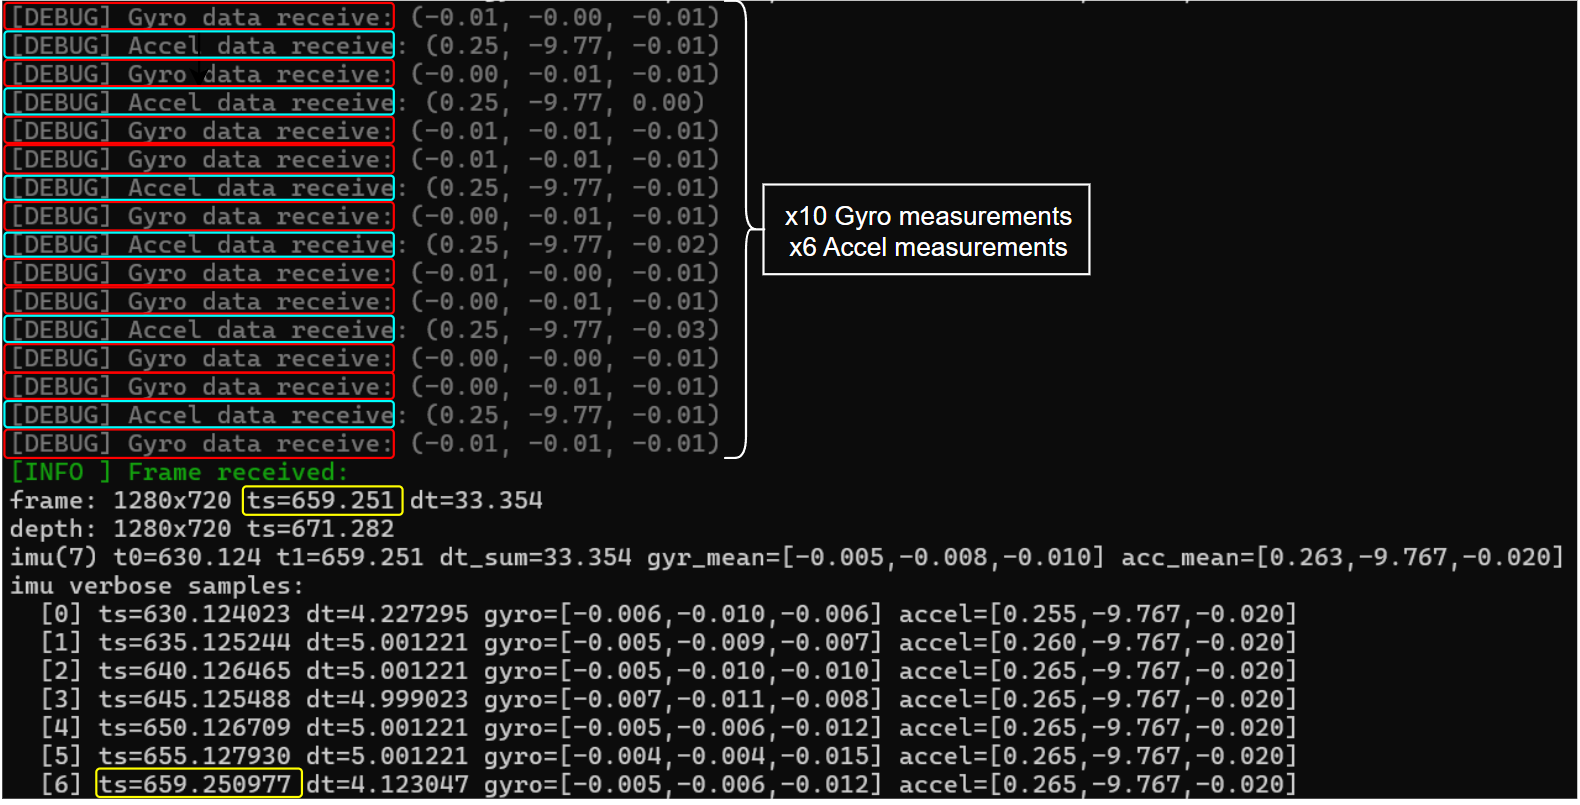
\includegraphics[scale=0.3]{images/source_manager_sync.png}}
\end{figure}

\section{Envío de comandos de velocidad}

Una vez calculado el comando de velocidad por el controlador, este debe enviarse al UAV para su ejecución. Dicho comando 
está compuesto por una velocidad lineal y una velocidad angular, expresadas en el sistema de referencia empleado por el 
algoritmo de navegación:

\begin{equation}
    \mathbf{u}
    =
    \begin{bmatrix}
        v_x &
        v_y &
        v_z &
        \omega_z
    \end{bmatrix}^{T},
\end{equation}

donde $v_x$, $v_y$ y $v_z$ representan las componentes de velocidad lineal, y $\omega_z$ corresponde a la velocidad angular 
alrededor del eje vertical del UAV.

El envío de comandos se realiza desde la estación de tierra hacia la plataforma aérea mediante comunicación UDP. Esta 
solución permite transmitir consignas de control con baja latencia, lo cual resulta fundamental en aplicaciones de 
navegación autónoma. En la plataforma aérea, la Jetson Nano recibe estos comandos, los interpreta y los reenvía al 
controlador de vuelo para que sean ejecutados por el UAV.

Para evitar comportamientos bruscos o no deseados, antes del envío se aplican límites máximos a las componentes de 
velocidad. Esta saturación puede expresarse como

\begin{equation}
\begin{aligned}
    \bar{v}_i
    &=
    \operatorname{sat}
    \left(
        v_i,
        v_{i,\max}
    \right)
    =
    \max
    \left(
        -v_{i,\max},
        \min
        \left(
            v_i,
            v_{i,\max}
        \right)
    \right),
    \qquad
    i \in \{x,y,z\},
    \\[2mm]
    \bar{\omega}_z
    &=
    \operatorname{sat}
    \left(
        \omega_z,
        \omega_{z,\max}
    \right)
    =
    \max
    \left(
        -\omega_{z,\max},
        \min
        \left(
            \omega_z,
            \omega_{z,\max}
        \right)
    \right).
\end{aligned}
\end{equation}

Por tanto, el comando finalmente enviado al UAV queda definido como

\begin{equation}
    \bar{\mathbf{u}}
    =
    \begin{bmatrix}
        \bar{v}_x &
        \bar{v}_y &
        \bar{v}_z &
        \bar{\omega}_z
    \end{bmatrix}^{T}.
\end{equation}

De esta forma, el sistema garantiza que las consignas enviadas al UAV se mantienen dentro de los límites dinámicos 
definidos para la plataforma. 
\chapter{Estimador de odometría Visual e inercial}

\section{Arquitectura}

El algoritmo de odometría visual-inercial implementado sigue una formulación robocéntrica basada conceptualmente en 
R-VIO2~\cite{huai2022square}. En este enfoque, la estimación no se realiza directamente respecto a un marco global fijo, 
sino respecto a un marco local asociado al movimiento del propio sensor. Esta elección permite mantener una ventana 
deslizante de estados relativos y actualizar el sistema mediante una matriz de información en forma \textit{square-root}. 
Aunque el diseño general se inspira en dicho trabajo, la implementación utilizada en este proyecto ha sido desarrollada 
de forma propia. La arquitectura del sistema se muestra en la Figura~\ref{fig:vio_arq}.


\begin{figure}[H]
    \ffigbox[\FBwidth] {
        \caption[Arquitectura del sistema de odometría visual-inercial.]{Arquitectura del sistema de odometría visual-inercial.}
        \label{fig:vio_arq}
    }
    {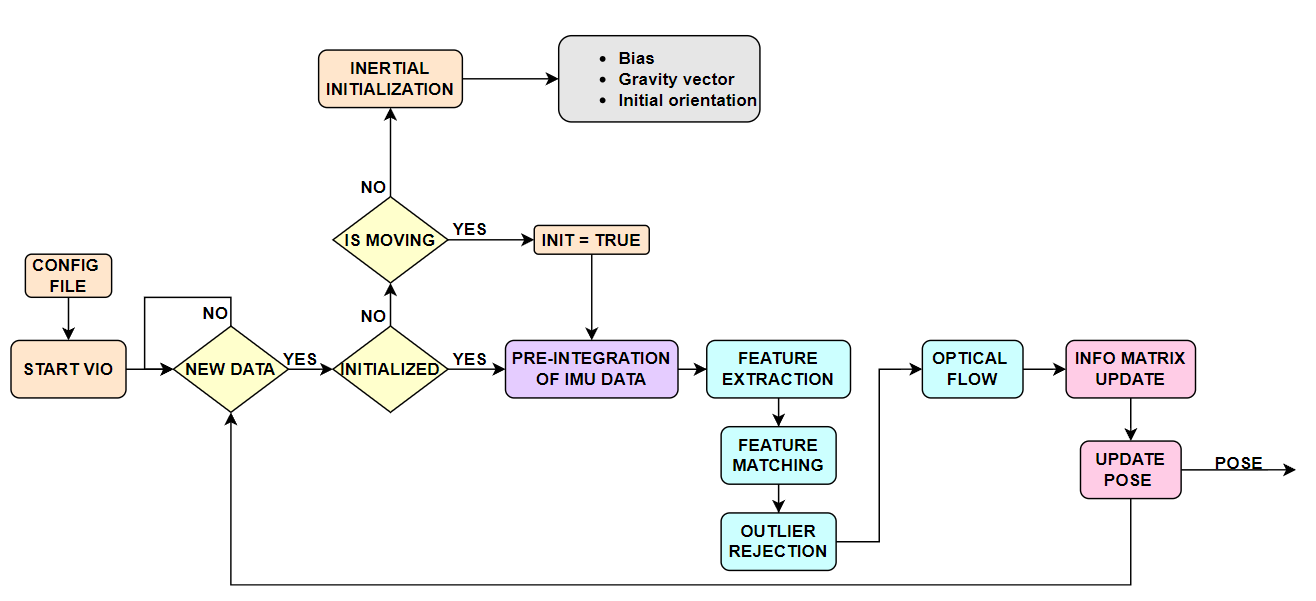
\includegraphics[scale=0.38]{images/vio_arquitecture.png}}
\end{figure}



El flujo principal del algoritmo se puede resumir en los siguientes pasos:

\begin{enumerate}[nosep]
    \item Se recibe un paquete, compuesto por una imagen RGB y una secuencia de medidas IMU sincronizadas con el intervalo de dos imágenes consecutivas.
    \item Si el sistema aún no ha sido inicializado, se estima la dirección de la gravedad y los sesgos iniciales de la IMU a partir de un intervalo en reposo.
    \item Se propaga el estado mediante pre-integracion inercial, generando un nuevo factor IMU y actualizando la matriz de información \textit{square-root}.
    \item Se predice la pose de la cámara a partir del estado propagado.
    \item Se realiza el seguimiento visual de características mediante flujo óptico KLT y se rechazan correspondencias erróneas mediante RANSAC.
    \item Se triangulan nuevas features usando parametrización de profundidad inversa.
    \item Se construyen los factores visuales y se incorporan al sistema mediante actualizaciones QR.
    \item Se aplica la corrección estimada al estado y se realiza la composición robocéntrica, cambiando el marco local de referencia al instante actual.
\end{enumerate}

\section{Inicialización del sistema}

La inicialización del sistema tiene como objetivo estimar las condiciones iniciales necesarias para comenzar la odometría visual-inercial. En concreto, se calculan tres magnitudes principales: la dirección inicial de la gravedad, el sesgo inicial del giróscopo y el sesgo inicial del acelerómetro. Estas variables son fundamentales, ya que el estimador necesita partir de una orientación coherente y de unas medidas inerciales corregidas antes de iniciar la propagación del estado.

El procedimiento se basa en detectar un intervalo inicial en el que la plataforma permanezca aproximadamente en reposo. Para ello, se analizan las muestras IMU recibidas y se estima el movimiento angular y el desplazamiento aproximado durante dicho intervalo. En primer lugar, se elimina de forma aproximada la componente de la gravedad de la aceleración medida y se acumulan las variaciones de orientación, velocidad y posición:

\begin{equation}
\begin{aligned}
    \Delta \boldsymbol{\theta}
    &=
    \sum_i
    \boldsymbol{\omega}_i \Delta t_i,
    \\
    \Delta \mathbf{v}
    &=
    \sum_i
    \mathbf{a}_i \Delta t_i,
    \\
    \Delta \mathbf{p}
    &=
    \sum_i
    \left(
        \Delta \mathbf{v}_i \Delta t_i
        +
        \frac{1}{2}
        \mathbf{a}_i \Delta t_i^2
    \right).
\end{aligned}
\end{equation}

Si la variación angular y el desplazamiento estimado son inferiores a los umbrales configurados, el sistema considera que el UAV todavía no se ha movido. En ese caso, las medidas de acelerómetro y giróscopo se acumulan para calcular una media más robusta. Además, se almacena la última imagen recibida, que será utilizada posteriormente para inicializar el sistema de seguimiento visual.

Cuando se detecta movimiento, el sistema deja de acumular medidas y calcula las condiciones iniciales. Si se han acumulado suficientes muestras, se calcula la media de las medidas inerciales. A partir de esta media se estima la dirección de la gravedad, el sesgo del giróscopo y el sesgo del acelerómetro:

\begin{equation}
\begin{aligned}
    \mathbf{g}
    &=
    \frac{\bar{\mathbf{a}}}
    {\left\|\bar{\mathbf{a}}\right\|},
    \\
    \mathbf{b}_g
    &=
    \bar{\boldsymbol{\omega}},
    \\
    \mathbf{b}_a
    &=
    \bar{\mathbf{a}}
    -
    g_0 \mathbf{g}.
\end{aligned}
\end{equation}

donde $\bar{\boldsymbol{\omega}}$ es la media de las velocidades angulares, $\bar{\mathbf{a}}$ es la media de las aceleraciones medidas, $g_0$ es el módulo de la gravedad y $\mathbf{g}$ es la dirección estimada de la gravedad. En caso de que la plataforma comience ya en movimiento y no exista un intervalo inicial en reposo, el sistema utiliza la última muestra disponible como estimación inicial, aunque en este caso los sesgos se inicializan a cero.

Una vez calculadas estas magnitudes, se inicializa el vector de estado local del estimador. Este vector contiene la orientación y posición iniciales, la dirección de la gravedad, la calibración extrínseca cámara-IMU, el desfase temporal entre sensores, la velocidad inicial y los sesgos de la IMU:

\begin{equation}
    \mathbf{x}_0
    =
    \left[
        \mathbf{q}_G,
        \mathbf{p}_G,
        \mathbf{g},
        \mathbf{q}_{CI},
        \mathbf{t}_{CI},
        t_d,
        \mathbf{v},
        \mathbf{b}_g,
        \mathbf{b}_a
    \right].
\end{equation}


La calibración extrínseca entre la cámara y la IMU se inicializa con los valores disponibles en la configuración, es decir, con la rotación $\mathbf{q}_{CI}$ y la traslación $\mathbf{t}_{CI}$. El desfase temporal inicial entre cámara e IMU se establece a cero. La velocidad inicial también se considera nula, mientras que los sesgos se inicializan con los valores estimados durante el intervalo en reposo.

Además del vector de estado, se inicializa la matriz de información local del estimador. Esta matriz introduce la confianza inicial sobre cada una de las variables del estado. Las variables conocidas con mayor precisión, como la pose inicial, se inicializan con una incertidumbre baja. En cambio, los parámetros de calibración cámara-IMU y el desfase temporal se inicializan con una incertidumbre dependiente de si existe o no una calibración previa conocida. Si dicha calibración está disponible, se asigna una confianza mayor; en caso contrario, se permite que el estimador corrija estos parámetros con mayor libertad durante la navegación.

Finalmente, se inicializa el módulo de seguimiento visual utilizando la última imagen almacenada durante la fase de reposo. Con ello se detectan las primeras características visuales y se fija la primera pose válida del sistema. A partir de este momento, el estimador queda marcado como inicializado y puede comenzar el proceso normal de propagación inercial, seguimiento visual y actualización del estado.

\section{Preintegración inercial}

La preintegración inercial permite condensar un conjunto de medidas IMU de alta frecuencia, tomadas entre dos fotogramas 
consecutivos, en una única restricción de movimiento. Esta técnica es especialmente útil en sistemas visual-inerciales, ya 
que evita tener que actualizar el estado completo del estimador con cada muestra de la IMU. En su lugar, las medidas 
inerciales se acumulan localmente y se incorporan posteriormente al sistema como un único factor entre dos instantes 
visuales~\cite{morris2024imu_preintegration}.

El punto de partida es el modelo de medida de una IMU. El giróscopo mide la velocidad angular afectada por un sesgo y por 
ruido blanco:

\begin{equation}
    \tilde{\boldsymbol{\omega}}_k
    =
    \boldsymbol{\omega}_k
    +
    \mathbf{b}_{g,k}
    +
    \boldsymbol{\eta}_{g,k},
\end{equation}

mientras que el acelerómetro mide la fuerza específica, también afectada por sesgo y ruido:

\begin{equation}
    \tilde{\mathbf{a}}_k
    =
    \mathbf{R}_{WB,k}^{T}
    \left(
        \mathbf{a}_{W,k}
        -
        \mathbf{g}_{W}
    \right)
    +
    \mathbf{b}_{a,k}
    +
    \boldsymbol{\eta}_{a,k}.
\end{equation}

En estas expresiones, $\tilde{\boldsymbol{\omega}}_k$ y $\tilde{\mathbf{a}}_k$ son las medidas proporcionadas por la IMU, $\mathbf{b}_{g,k}$ y $\mathbf{b}_{a,k}$ son los sesgos del giróscopo y del acelerómetro, $\boldsymbol{\eta}_{g,k}$ y $\boldsymbol{\eta}_{a,k}$ representan el ruido de medida, $\mathbf{R}_{WB,k}$ es la rotación del cuerpo respecto al sistema global y $\mathbf{g}_{W}$ es el vector de gravedad.

Corrigiendo las medidas con los sesgos estimados, se obtiene

\begin{equation}
    \boldsymbol{\omega}_k
    =
    \tilde{\boldsymbol{\omega}}_k
    -
    \mathbf{b}_{g,k},
    \qquad
    \mathbf{a}_k
    =
    \tilde{\mathbf{a}}_k
    -
    \mathbf{b}_{a,k}.
\end{equation}

A partir de estas medidas corregidas, el modelo cinemático continuo de la IMU puede escribirse como

\begin{equation}
\begin{aligned}
    \dot{\mathbf{R}}_{WB}
    &=
    \mathbf{R}_{WB}
    \left[
        \boldsymbol{\omega}
    \right]_{\times},
    \\
    \dot{\mathbf{p}}_{W}
    &=
    \mathbf{v}_{W},
    \\
    \dot{\mathbf{v}}_{W}
    &=
    \mathbf{R}_{WB}
    \mathbf{a}
    +
    \mathbf{g}_{W},
\end{aligned}
\end{equation}

donde $\left[\cdot\right]_{\times}$ representa la matriz antisimétrica asociada al producto vectorial.

En una integración directa, cada muestra de la IMU se utilizaría para propagar orientación, posición y velocidad en el sistema global. Sin embargo, esto obliga a trabajar continuamente con el estado completo del estimador y con la gravedad expresada en el marco global. La idea principal de la preintegración consiste en acumular las medidas IMU en un marco local asociado al instante inicial del intervalo. De este modo, se calculan tres incrementos relativos:

\begin{equation}
    \Delta \mathbf{R}_{ij},
    \qquad
    \Delta \mathbf{p}_{ij},
    \qquad
    \Delta \mathbf{v}_{ij},
\end{equation}

que representan, respectivamente, el incremento de rotación, posición y velocidad entre los instantes $i$ y $j$.

Al inicio de cada intervalo de preintegración se inicializan los incrementos como

\begin{equation}
\begin{aligned}
    \Delta \mathbf{R}_{ij}
    &=
    \mathbf{I},
    \\
    \Delta \mathbf{p}_{ij}
    &=
    \mathbf{0},
    \\
    \Delta \mathbf{v}_{ij}
    &=
    \mathbf{0},
    \\
    \Delta t_{ij}
    &=
    0.
\end{aligned}
\end{equation}

Para cada muestra IMU recibida dentro del intervalo, con paso temporal $\delta t_k$, se calculan los incrementos elementales:

\begin{equation}
\begin{aligned}
    \delta \mathbf{R}_{k}
    &=
    \operatorname{Exp}
    \left(
        \left[
            \boldsymbol{\omega}_k
        \right]_{\times}
        \delta t_k
    \right),
    \\
    \delta \mathbf{v}_{k}
    &=
    \mathbf{a}_k
    \delta t_k,
    \\
    \delta \mathbf{p}_{k}
    &=
    \frac{1}{2}
    \mathbf{a}_k
    \delta t_k^2.
\end{aligned}
\end{equation}

Estos incrementos se acumulan de forma recursiva mediante

\begin{equation}
\begin{aligned}
    \Delta \mathbf{p}_{ij}
    &\leftarrow
    \Delta \mathbf{p}_{ij}
    +
    \Delta \mathbf{v}_{ij}
    \delta t_k
    +
    \Delta \mathbf{R}_{ij}
    \delta \mathbf{p}_{k},
    \\
    \Delta \mathbf{v}_{ij}
    &\leftarrow
    \Delta \mathbf{v}_{ij}
    +
    \Delta \mathbf{R}_{ij}
    \delta \mathbf{v}_{k},
    \\
    \Delta \mathbf{R}_{ij}
    &\leftarrow
    \Delta \mathbf{R}_{ij}
    \delta \mathbf{R}_{k},
    \\
    \Delta t_{ij}
    &\leftarrow
    \Delta t_{ij}
    +
    \delta t_k.
\end{aligned}
\label{eq:preintegracion_imu}
\end{equation}

La gravedad no se incluye directamente en los incrementos preintegrados, ya que depende del sistema de referencia global y de la pose del instante inicial. Por ello, se añade posteriormente al formular la relación entre dos estados consecutivos. Dado un estado en el instante $i$, el estado predicho en el instante $j$ se obtiene como

\begin{equation}
\begin{aligned}
    \mathbf{R}_{WB,j}
    &=
    \mathbf{R}_{WB,i}
    \Delta \mathbf{R}_{ij},
    \\
    \mathbf{p}_{W,j}
    &=
    \mathbf{p}_{W,i}
    +
    \mathbf{v}_{W,i}
    \Delta t_{ij}
    +
    \frac{1}{2}
    \mathbf{g}_{W}
    \Delta t_{ij}^{2}
    +
    \mathbf{R}_{WB,i}
    \Delta \mathbf{p}_{ij},
    \\
    \mathbf{v}_{W,j}
    &=
    \mathbf{v}_{W,i}
    +
    \mathbf{g}_{W}
    \Delta t_{ij}
    +
    \mathbf{R}_{WB,i}
    \Delta \mathbf{v}_{ij}.
\end{aligned}
\end{equation}

De forma equivalente, los incrementos preintegrados pueden interpretarse como una medida relativa entre los estados $i$ y $j$:

\begin{equation}
\begin{aligned}
    \Delta \mathbf{R}_{ij}
    &=
    \mathbf{R}_{WB,i}^{T}
    \mathbf{R}_{WB,j},
    \\
    \Delta \mathbf{p}_{ij}
    &=
    \mathbf{R}_{WB,i}^{T}
    \left(
        \mathbf{p}_{W,j}
        -
        \mathbf{p}_{W,i}
        -
        \mathbf{v}_{W,i}
        \Delta t_{ij}
        -
        \frac{1}{2}
        \mathbf{g}_{W}
        \Delta t_{ij}^{2}
    \right),
    \\
    \Delta \mathbf{v}_{ij}
    &=
    \mathbf{R}_{WB,i}^{T}
    \left(
        \mathbf{v}_{W,j}
        -
        \mathbf{v}_{W,i}
        -
        \mathbf{g}_{W}
        \Delta t_{ij}
    \right).
\end{aligned}
\end{equation}

Estas ecuaciones permiten construir un residuo inercial que relaciona dos estados consecutivos del estimador:

\begin{equation}
    \mathbf{r}_{imu}
    =
    \begin{bmatrix}
        \mathbf{r}_{R} \\
        \mathbf{r}_{p} \\
        \mathbf{r}_{v}
    \end{bmatrix},
\end{equation}

con

\begin{equation}
\begin{aligned}
    \mathbf{r}_{R}
    &=
    \operatorname{Log}
    \left(
        \Delta \mathbf{R}_{ij}^{T}
        \mathbf{R}_{WB,i}^{T}
        \mathbf{R}_{WB,j}
    \right),
    \\
    \mathbf{r}_{p}
    &=
    \mathbf{R}_{WB,i}^{T}
    \left(
        \mathbf{p}_{W,j}
        -
        \mathbf{p}_{W,i}
        -
        \mathbf{v}_{W,i}
        \Delta t_{ij}
        -
        \frac{1}{2}
        \mathbf{g}_{W}
        \Delta t_{ij}^{2}
    \right)
    -
    \Delta \mathbf{p}_{ij},
    \\
    \mathbf{r}_{v}
    &=
    \mathbf{R}_{WB,i}^{T}
    \left(
        \mathbf{v}_{W,j}
        -
        \mathbf{v}_{W,i}
        -
        \mathbf{g}_{W}
        \Delta t_{ij}
    \right)
    -
    \Delta \mathbf{v}_{ij}.
\end{aligned}
\end{equation}

Como los incrementos preintegrados dependen de los sesgos utilizados durante su cálculo, una variación posterior de dichos sesgos debe corregirse. Para ello, se emplea una aproximación de primer orden:

\begin{equation}
\begin{aligned}
    \Delta \mathbf{R}_{ij}
    &\leftarrow
    \Delta \mathbf{R}_{ij}
    \operatorname{Exp}
    \left(
        \mathbf{J}_{\Delta R}^{b_g}
        \delta \mathbf{b}_{g}
    \right),
    \\
    \Delta \mathbf{p}_{ij}
    &\leftarrow
    \Delta \mathbf{p}_{ij}
    +
    \mathbf{J}_{\Delta p}^{b_g}
    \delta \mathbf{b}_{g}
    +
    \mathbf{J}_{\Delta p}^{b_a}
    \delta \mathbf{b}_{a},
    \\
    \Delta \mathbf{v}_{ij}
    &\leftarrow
    \Delta \mathbf{v}_{ij}
    +
    \mathbf{J}_{\Delta v}^{b_g}
    \delta \mathbf{b}_{g}
    +
    \mathbf{J}_{\Delta v}^{b_a}
    \delta \mathbf{b}_{a}.
\end{aligned}
\end{equation}

La preintegración inercial transforma, por tanto, una secuencia de medidas IMU de alta frecuencia en una única medida relativa entre dos fotogramas. Esto reduce el coste computacional, facilita la fusión con sensores visuales y permite que el estimador utilice las medidas inerciales como restricciones dentro del problema de optimización visual-inercial.

\section{Propagación de incertidumbre}

La covarianza asociada a la propagación inercial se actualiza mediante el modelo linealizado

\begin{equation}
    \boldsymbol{\Phi}_i
    =
    \mathbf{I}
    +
    \Delta t_i
    \mathbf{F}_i,
\end{equation}

\begin{equation}
    \mathbf{Q}_i
    =
    \Delta t_i
    \mathbf{G}_i
    \boldsymbol{\Sigma}_{imu}
    \mathbf{G}_i^{T},
\end{equation}

\begin{equation}
    \mathbf{P}_i
    =
    \boldsymbol{\Phi}_i
    \mathbf{P}_{i-1}
    \boldsymbol{\Phi}_i^{T}
    +
    \mathbf{Q}_i.
\end{equation}

La matriz de ruido de la IMU se define como

\begin{equation}
    \boldsymbol{\Sigma}_{imu}
    =
    \operatorname{diag}
    \left(
        \boldsymbol{\sigma}_{g}^{2},
        \boldsymbol{\sigma}_{bg}^{2},
        \boldsymbol{\sigma}_{a}^{2},
        \boldsymbol{\sigma}_{ba}^{2}
    \right),
\end{equation}

donde $\boldsymbol{\sigma}_{g}$ y $\boldsymbol{\sigma}_{a}$ son las desviaciones típicas del ruido del giróscopo y acelerómetro, y $\boldsymbol{\sigma}_{bg}$ y $\boldsymbol{\sigma}_{ba}$ las correspondientes caminatas aleatorias de sus sesgos.

A partir de la covarianza propagada se obtiene la matriz de información

\begin{equation}
    \boldsymbol{\Lambda}
    =
    \mathbf{P}^{-1},
\end{equation}

y su factorización de Cholesky

\begin{equation}
    \boldsymbol{\Lambda}
    =
    \mathbf{L}
    \mathbf{L}^{T}.
\end{equation}

El factor inercial introducido en el sistema se construye como

\begin{equation}
    \mathbf{H}_{imu}
    =
    \mathbf{L}^{T}
    \begin{bmatrix}
        \boldsymbol{\Psi}_{p} &
        \boldsymbol{\Psi}_{v,b} &
        -\mathbf{I}
    \end{bmatrix},
\end{equation}

donde $\boldsymbol{\Psi}$ es la matriz de transición acumulada durante la integración.

\section{Seguimiento visual}

El módulo \texttt{Tracker} realiza el seguimiento de características entre imágenes consecutivas. En primer lugar, la imagen se convierte a escala de grises y, opcionalmente, se aplican filtrado y ecualización adaptativa. A continuación, se detectan nuevas características mediante el criterio de Shi-Tomasi:

\begin{equation}
    q(\mathbf{u})
    =
    \min
    \left(
        \lambda_1,
        \lambda_2
    \right),
\end{equation}

donde $\lambda_1$ y $\lambda_2$ son los autovalores de la matriz de segundo momento local de la imagen. Solo se aceptan puntos con calidad suficiente y separados una distancia mínima en la imagen.

El seguimiento entre imágenes se realiza mediante flujo óptico KLT, que asume constancia de brillo:

\begin{equation}
    I_k(\mathbf{u})
    \simeq
    I_{k+1}
    \left(
        \mathbf{u}
        +
        \Delta \mathbf{u}
    \right).
\end{equation}

El desplazamiento de cada característica se estima minimizando

\begin{equation}
    \Delta \mathbf{u}^{*}
    =
    \arg\min_{\Delta \mathbf{u}}
    \sum_{\mathbf{s} \in \Omega}
    \left[
        I_{k+1}
        \left(
            \mathbf{u}
            +
            \mathbf{s}
            +
            \Delta \mathbf{u}
        \right)
        -
        I_k
        \left(
            \mathbf{u}
            +
            \mathbf{s}
        \right)
    \right]^2.
\end{equation}

Después del seguimiento, los puntos se corrigen de distorsión y se expresan como rayos normalizados:

\begin{equation}
    \mathbf{m}
    =
    \frac{
        \begin{bmatrix}
            x_n \\
            y_n \\
            1
        \end{bmatrix}
    }
    {
        \left\|
        \begin{bmatrix}
            x_n \\
            y_n \\
            1
        \end{bmatrix}
        \right\|
    }.
\end{equation}

\section{Rechazo de outliers mediante RANSAC}

Para eliminar correspondencias erróneas, el código usa un RANSAC basado en la restricción epipolar. Dada una rotación relativa estimada $\mathbf{R}$, se calcula una matriz esencial de la forma

\begin{equation}
    \mathbf{E}
    =
    \left[
    \mathbf{t}
    \right]_{\times}
    \mathbf{R}.
\end{equation}

La traslación se parametriza mediante dos ángulos $\alpha$ y $\beta$:

\begin{equation}
    \mathbf{t}
    =
    \begin{bmatrix}
        \sin\beta\cos\alpha \\
        \cos\beta \\
        -\sin\beta\sin\alpha
    \end{bmatrix}.
\end{equation}

Para cada correspondencia se evalúa la restricción epipolar

\begin{equation}
    \mathbf{m}_{2}^{T}
    \mathbf{E}
    \mathbf{m}_{1}
    =
    0.
\end{equation}

El error algebraico se define como

\begin{equation}
    e_{alg}
    =
    \left(
        \mathbf{m}_{2}^{T}
        \mathbf{E}
        \mathbf{m}_{1}
    \right)^2.
\end{equation}

Cuando se activa el criterio de Sampson, se emplea

\begin{equation}
    e_{samp}
    =
    \frac{
        \left(
            \mathbf{m}_{2}^{T}
            \mathbf{E}
            \mathbf{m}_{1}
        \right)^2
    }
    {
        \left(
            \mathbf{E}\mathbf{m}_{1}
        \right)_1^2
        +
        \left(
            \mathbf{E}\mathbf{m}_{1}
        \right)_2^2
        +
        \left(
            \mathbf{E}^{T}\mathbf{m}_{2}
        \right)_1^2
        +
        \left(
            \mathbf{E}^{T}\mathbf{m}_{2}
        \right)_2^2
    }.
\end{equation}

Una correspondencia se acepta como inlier si

\begin{equation}
    e < e_{\max},
\end{equation}

donde $e_{\max}$ es el umbral configurado para el error algebraico o para el error de Sampson.

\section{Triangulación por profundidad inversa}

Las características visuales se parametrizan mediante profundidad inversa. Para una característica observada por primera vez, se define

\begin{equation}
    \boldsymbol{\lambda}
    =
    \begin{bmatrix}
        \phi \\
        \psi \\
        \rho
    \end{bmatrix},
\end{equation}

donde $\phi$ es el ángulo de elevación, $\psi$ el ángulo de acimut y $\rho$ la profundidad inversa.

El vector unitario asociado a la observación inicial es

\begin{equation}
    \mathbf{e}
    \left(
        \phi,
        \psi
    \right)
    =
    \begin{bmatrix}
        \cos\phi \sin\psi \\
        \sin\phi \\
        \cos\phi \cos\psi
    \end{bmatrix}.
\end{equation}

La inicialización usada en el código es

\begin{equation}
    \phi_0
    =
    \arctan2
    \left(
        y_0,
        \sqrt{x_0^2+1}
    \right),
\end{equation}

\begin{equation}
    \psi_0
    =
    \arctan2
    \left(
        x_0,
        1
    \right),
\end{equation}

\begin{equation}
    \rho_0 = 0.
\end{equation}

Para una observación $i$, el punto proyectado en la cámara se calcula como

\begin{equation}
    \mathbf{h}_i
    =
    \mathbf{R}_i
    \mathbf{e}
    \left(
        \phi,
        \psi
    \right)
    +
    \rho
    \mathbf{t}_i.
\end{equation}

La predicción de la medida normalizada es

\begin{equation}
    \hat{\mathbf{z}}_i
    =
    \begin{bmatrix}
        h_{x,i}/h_{z,i} \\
        h_{y,i}/h_{z,i}
    \end{bmatrix}.
\end{equation}

El residuo visual queda definido como

\begin{equation}
    \mathbf{e}_i
    =
    \mathbf{z}_i
    -
    \hat{\mathbf{z}}_i.
\end{equation}

La matriz jacobiana de la proyección es

\begin{equation}
    \mathbf{H}_{\pi}
    =
    \begin{bmatrix}
        1/h_z & 0 & -h_x/h_z^2 \\
        0 & 1/h_z & -h_y/h_z^2
    \end{bmatrix}.
\end{equation}

La derivada del vector direccional respecto a $\phi$ y $\psi$ es

\begin{equation}
    \frac{\partial \mathbf{e}}{\partial \left[\phi,\psi\right]}
    =
    \begin{bmatrix}
        -\sin\phi\sin\psi & \cos\phi\cos\psi \\
        \cos\phi & 0 \\
        -\sin\phi\cos\psi & -\cos\phi\sin\psi
    \end{bmatrix}.
\end{equation}

Por tanto, el jacobiano de la observación respecto a la parametrización de profundidad inversa es

\begin{equation}
    \mathbf{H}_{\lambda,i}
    =
    \mathbf{H}_{\pi}
    \begin{bmatrix}
        \mathbf{R}_i
        \frac{\partial \mathbf{e}}{\partial \left[\phi,\psi\right]}
        &
        \mathbf{t}_i
    \end{bmatrix}.
\end{equation}

La triangulación se refina mediante Levenberg-Marquardt resolviendo

\begin{equation}
    \left(
        \mathbf{H}^{T}
        \boldsymbol{\Sigma}^{-1}
        \mathbf{H}
        +
        \lambda
        \operatorname{diag}
        \left(
            \mathbf{H}^{T}
            \boldsymbol{\Sigma}^{-1}
            \mathbf{H}
        \right)
    \right)
    \Delta \boldsymbol{\lambda}
    =
    \mathbf{H}^{T}
    \boldsymbol{\Sigma}^{-1}
    \mathbf{e}.
\end{equation}

La actualización de la característica es

\begin{equation}
    \boldsymbol{\lambda}
    \leftarrow
    \boldsymbol{\lambda}
    +
    \Delta \boldsymbol{\lambda}.
\end{equation}

La triangulación se acepta únicamente si

\begin{equation}
    \rho > 0,
    \qquad
    \left|\phi\right| < \frac{\pi}{2},
    \qquad
    \left|\psi\right| < \frac{\pi}{2}.
\end{equation}

\section{Factor visual y eliminación de la característica}

Para una característica observada en varias imágenes, el modelo linealizado puede escribirse como

\begin{equation}
    \mathbf{e}
    \simeq
    \mathbf{H}_{x}
    \delta \mathbf{x}
    +
    \mathbf{H}_{\lambda}
    \delta \boldsymbol{\lambda}
    +
    \mathbf{n}.
\end{equation}

Como la característica no forma parte del estado principal en los factores de tipo \textit{pose-only}, se elimina mediante una descomposición QR:

\begin{equation}
    \mathbf{H}_{\lambda}
    =
    \begin{bmatrix}
        \mathbf{Q}_1 &
        \mathbf{Q}_2
    \end{bmatrix}
    \begin{bmatrix}
        \mathbf{R}_{\lambda} \\
        \mathbf{0}
    \end{bmatrix}.
\end{equation}

Proyectando el residuo sobre el espacio nulo de la característica se obtiene

\begin{equation}
    \mathbf{e}^{\prime}
    =
    \mathbf{Q}_2^{T}
    \mathbf{e},
\end{equation}

\begin{equation}
    \mathbf{H}^{\prime}
    =
    \mathbf{Q}_2^{T}
    \mathbf{H}_{x}.
\end{equation}

El coste visual resultante es

\begin{equation}
    C_{cam}
    =
    \left\|
        \mathbf{H}^{\prime}
        \delta \mathbf{x}
        -
        \mathbf{e}^{\prime}
    \right\|_{\boldsymbol{\Sigma}_{cam}}^2.
\end{equation}

Este procedimiento coincide con la idea de eliminación por espacio nulo utilizada en formulaciones visual-inerciales de ventana deslizante, y está alineado con la formulación \textit{square-root} descrita en R-VIO2~\cite{huai2022square}.

\section{Actualización \textit{square-root}}

El sistema mantiene una matriz de información en forma \textit{square-root}, almacenada como \texttt{LocalFactor}. El problema de mínimos cuadrados en cada actualización se expresa como

\begin{equation}
    \delta \mathbf{x}^{*}
    =
    \arg\min_{\delta \mathbf{x}}
    \left\|
        \mathbf{S}
        \delta \mathbf{x}
        -
        \mathbf{r}
    \right\|^2
    +
    \left\|
        \mathbf{H}
        \delta \mathbf{x}
        -
        \mathbf{e}
    \right\|^2,
\end{equation}

donde $\mathbf{S}$ es el factor \textit{square-root} previo, $\mathbf{r}$ es el término independiente acumulado, $\mathbf{H}$ es el nuevo jacobiano y $\mathbf{e}$ el nuevo residuo.

La actualización se realiza apilando el factor previo y las nuevas medidas:

\begin{equation}
    \begin{bmatrix}
        \mathbf{S} \\
        \mathbf{H}
    \end{bmatrix}
    \delta \mathbf{x}
    =
    \begin{bmatrix}
        \mathbf{r} \\
        \mathbf{e}
    \end{bmatrix}.
\end{equation}

A continuación, se aplica QR mediante rotaciones de Givens:

\begin{equation}
    \mathbf{Q}^{T}
    \begin{bmatrix}
        \mathbf{S} \\
        \mathbf{H}
    \end{bmatrix}
    =
    \begin{bmatrix}
        \mathbf{S}^{+} \\
        \mathbf{0}
    \end{bmatrix},
\end{equation}

\begin{equation}
    \mathbf{Q}^{T}
    \begin{bmatrix}
        \mathbf{r} \\
        \mathbf{e}
    \end{bmatrix}
    =
    \begin{bmatrix}
        \mathbf{r}^{+} \\
        \boldsymbol{\epsilon}
    \end{bmatrix}.
\end{equation}

El nuevo problema reducido queda como

\begin{equation}
    \delta \mathbf{x}^{*}
    =
    \arg\min_{\delta \mathbf{x}}
    \left\|
        \mathbf{S}^{+}
        \delta \mathbf{x}
        -
        \mathbf{r}^{+}
    \right\|^2.
\end{equation}

La corrección del estado se obtiene por sustitución hacia atrás:

\begin{equation}
    \mathbf{S}^{+}
    \delta \mathbf{x}^{*}
    =
    \mathbf{r}^{+}.
\end{equation}

\section{Actualización del estado}

La corrección rotacional se aplica mediante una perturbación de cuaternión. Para una corrección angular $\delta\boldsymbol{\theta}$, el cuaternión incremental se aproxima como

\begin{equation}
    \delta \mathbf{q}
    =
    \begin{bmatrix}
        \frac{1}{2}\delta\boldsymbol{\theta} \\
        \sqrt{
            1
            -
            \frac{1}{4}
            \left\|
            \delta\boldsymbol{\theta}
            \right\|^2
        }
    \end{bmatrix}.
\end{equation}

La orientación se actualiza mediante

\begin{equation}
    \mathbf{q}^{+}
    =
    \delta \mathbf{q}
    \otimes
    \mathbf{q}.
\end{equation}

Las variables euclídeas se actualizan de forma aditiva:

\begin{equation}
    \mathbf{p}^{+}
    =
    \mathbf{p}
    +
    \delta \mathbf{p},
\end{equation}

\begin{equation}
    \mathbf{v}^{+}
    =
    \mathbf{v}
    +
    \delta \mathbf{v},
\end{equation}

\begin{equation}
    \mathbf{b}_{g}^{+}
    =
    \mathbf{b}_{g}
    +
    \delta \mathbf{b}_{g},
    \qquad
    \mathbf{b}_{a}^{+}
    =
    \mathbf{b}_{a}
    +
    \delta \mathbf{b}_{a}.
\end{equation}

\section{Composición robocéntrica}

Una vez aplicada la corrección, el estimador cambia el marco de referencia local al instante actual. Esta operación es la composición robocéntrica del estado. Si $\mathbf{R}_k$ y $\mathbf{p}_k$ representan la pose relativa más reciente, el nuevo estado global se calcula como

\begin{equation}
    \mathbf{R}_{kG}
    =
    \mathbf{R}_k
    \mathbf{R}_{G},
\end{equation}

\begin{equation}
    \mathbf{p}_{kG}
    =
    \mathbf{R}_k
    \left(
        \mathbf{p}_{G}
        -
        \mathbf{p}_{k}
    \right),
\end{equation}

\begin{equation}
    \mathbf{g}_{k}
    =
    \mathbf{R}_k
    \mathbf{g}.
\end{equation}

Después de esta composición, el nuevo marco robocéntrico queda fijado en la pose actual de la IMU. Este cambio de referencia mantiene acotado el problema de estimación y permite trabajar con poses relativas dentro de la ventana deslizante.

Las características inicializadas en profundidad inversa se transforman a coordenadas globales mediante

\begin{equation}
    \mathbf{p}_{f}^{G}
    =
    \mathbf{R}_{kG}^{T}
    \left(
        \frac{1}{\rho}
        \mathbf{R}_{IC}
        \mathbf{e}
        \left(
            \phi,
            \psi
        \right)
        +
        \mathbf{t}_{IC}
        -
        \mathbf{p}_{kG}
    \right).
\end{equation}

\section{Salida del estimador}

La salida final del estimador contiene la pose, la velocidad y las medidas inerciales corregidas por sesgo. La velocidad expresada en el marco global se calcula como

\begin{equation}
    \mathbf{v}_{G}
    =
    \mathbf{R}_{G}^{T}
    \mathbf{v}_{k}.
\end{equation}

Las medidas IMU corregidas se obtienen mediante

\begin{equation}
    \boldsymbol{\omega}_{corr}
    =
    \boldsymbol{\omega}_{m}
    -
    \mathbf{b}_{g},
\end{equation}

\begin{equation}
    \mathbf{a}_{corr}
    =
    \mathbf{a}_{m}
    -
    \mathbf{b}_{a}.
\end{equation}

Estas magnitudes se almacenan en la estructura de salida \texttt{StateOut}, junto con la pose estimada y la marca temporal correspondiente.


\chapter{Evitación de obstáculos}

La evitación de obstáculos desarrollada en este proyecto se apoya en el 
trabajo realizado previamente en el proyecto de investigación tutelado~\cite{estudio-nav2D}. En dicho 
estudio se analizó la viabilidad de implementar un sistema de evitación visual de obstáculos para drones de bajo 
coste empleando únicamente una cámara monocular RGB. Esta restricción imponía dos requisitos fundamentales: extraer información geométrica 
suficiente a partir de una única imagen y mantener una velocidad de procesamiento compatible con una aplicación en tiempo real.

El trabajo previo se centró principalmente en el estudio comparativo de distintos modelos de estimación 
de profundidad monocular y en la definición de una arquitectura de software capaz de ejecutarlos de forma 
eficiente. Para ello se evaluaron diferentes alternativas, entre ellas MiDaS~\cite{Ranftl2020}, Depth 
Anything~\cite{cheng2024depthanything} y otros modelos recientes de estimación de profundidad, valorando 
aspectos como la velocidad de inferencia, la estabilidad temporal, la precisión relativa de la 
profundidad y la posibilidad de integración en una arquitectura acelerada. Asimismo, se estudió 
el uso de modelos en formato ONNX~\cite{onnx_repo}, junto con técnicas de optimización basadas en 
ejecución multihilo y aceleración mediante GPU, con el objetivo de reducir la latencia total del 
sistema.

Aunque los resultados obtenidos demostraron la viabilidad general del enfoque, también pusieron de 
manifiesto algunas limitaciones importantes. La principal dificultad residía en que los estimadores de 
profundidad relativa no proporcionan directamente una distancia métrica absoluta, por lo que no siempre 
resulta trivial distinguir entre un obstáculo realmente peligroso y una variación de profundidad sin 
relevancia para la navegación.

El algoritmo desarrollado en este nuevo proyecto parte de esas conclusiones y propone una arquitectura 
de evitación más robusta. En lugar de basarse únicamente en el gradiente global del mapa de profundidad, 
se emplea un estimador más avanzado, \textit{Depth Anything 3}~\cite{overview-da}, y se añade una etapa 
específica de postprocesado orientada a la toma de decisiones. Esta etapa analiza la distribución de 
profundidad mediante segmentación y regiones de interés. De esta forma, el sistema no solo estima hacia 
dónde conviene desplazar la referencia lateral de evasión, sino que también determina si la situación requiere realmente una 
maniobra de evasión.

\section{Arquitectura}
\begin{figure}[H]
    \centering
    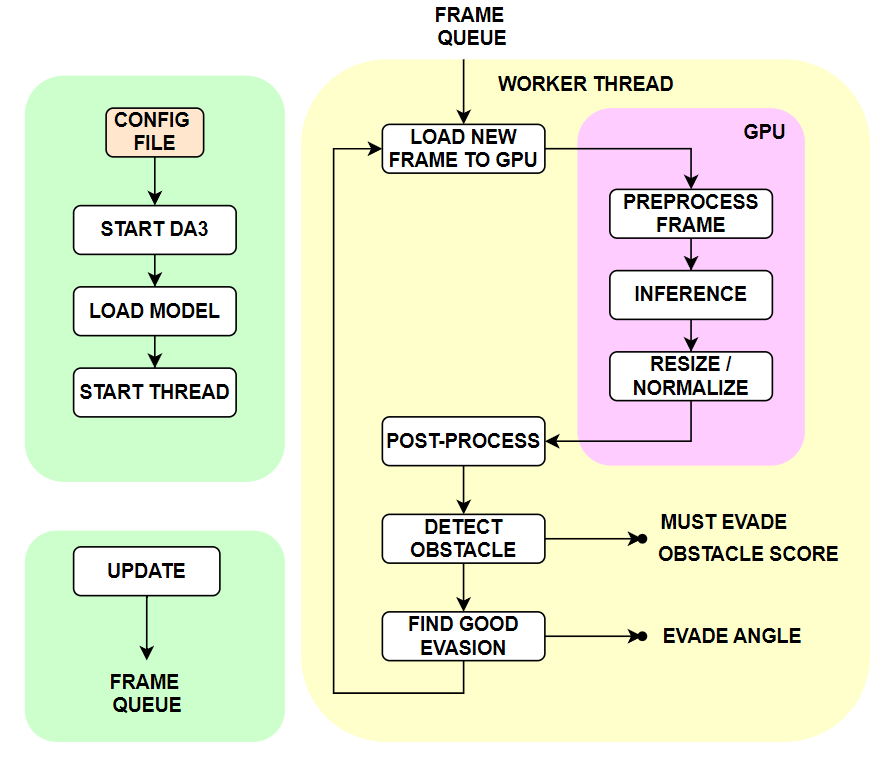
\includegraphics[width=1\textwidth]{images/depth_arq.png}
    \caption{Arquitectura del evitador de obstáculos. Fuente: Elaboración propia}
    \label{fig:evit_obs_arq}
\end{figure}

Como se observa en la Figura~\ref{fig:evit_obs_arq}, se propone una arquitectura acelerada por hardware, haciendo uso de 
la GPU y de CUDA tanto para ejecutar la inferencia del modelo como para realizar las operaciones de procesado mediante 
OpenCV~\cite{opencv_repo}.

En este módulo se distingue una primera etapa de inicialización, encargada de preparar el sistema, cargar el modelo 
utilizado y lanzar el hilo responsable de gestionar la comunicación con la GPU y calcular las diferentes métricas 
empleadas para la detección y evitación de obstáculos.

El funcionamiento general es sencillo: el hilo de trabajo (\textit{worker thread}) se encarga de realizar todo el proceso capturando 
siempre la imagen más reciente disponible en una cola interna. Dicha cola se actualiza cada vez que se recibe un nuevo 
\textit{fotograma} procedente de la cámara del UAV.

La salida principal del módulo se compone de tres parámetros:

\begin{enumerate}
    \item \texttt{evade\_angle} (\textit{float}): ángulo en 2D, expresado en coordenadas de imagen, que apunta hacia la 
    mejor dirección encontrada para evitar los obstáculos presentes en la escena.
    \item \texttt{obstacle\_score} (\textit{float}): indicador de riesgo asociado a la presencia de un obstáculo. Cuanto 
    mayor es su valor, mayor es la confianza del sistema en que existe un obstáculo cercano en la zona de avance.
    \item \texttt{must\_evade} (\textit{bool}): variable booleana encargada de indicar al planificador local cuándo debe 
    utilizar el ángulo de evasión y la puntuación de obstáculo calculados por el módulo.
\end{enumerate}

\section{Estimador de profundidad}
\subsection{Modelos y estudio de eficiencia}

Existen múltiples modelos de estimación de profundidad monocular, aunque no todos son adecuados para una arquitectura en 
tiempo real. Muchos de ellos presentan una elevada carga computacional. Por este motivo, en el proyecto 
previo~\cite{estudio-nav2D} se realizó un primer descarte de alternativas, atendiendo principalmente a la calidad de la 
profundidad estimada, la estabilidad visual entre fotogramas y la viabilidad de ejecución en tiempo real.

Tras dicho estudio inicial, las familias de modelos más prometedoras fueron MiDaS~\cite{Ranftl2020} y 
Depth Anything~\cite{cheng2024depthanything}. MiDaS destacaba por su robustez y por disponer de versiones relativamente 
ligeras, mientras que Depth Anything ofrecía una mejor generalización en escenas diversas y una estimación de profundidad 
visualmente más consistente. A partir de esta selección previa, en este proyecto se llevó a cabo un análisis más exhaustivo 
centrado en la eficiencia de inferencia, comparando distintos motores de ejecución, variantes de tamaño de los modelos y 
diferencias entre CPU y GPU.

El objetivo de esta comparación no era únicamente determinar qué modelo ofrecía mejores mapas de profundidad, sino 
seleccionar una configuración que permitiera integrar la estimación de profundidad dentro del sistema completo de 
evitación de obstáculos. Para ello se evaluaron principalmente dos motores de inferencia: OpenCV DNN~\cite{opencv_repo} y 
ONNX Runtime~\cite{onnx_repo}. Además, se comparó la ejecución sobre CPU y sobre GPU, ya que la arquitectura final del 
sistema debía aprovechar la aceleración por hardware disponible.

Las pruebas se realizaron sobre secuencias de 400 fotogramas, midiendo el tiempo medio, mínimo y la frecuencia de inferencia en fotogramas/s. La 
Tabla~\ref{tab:depth_models_efficiency} resume los resultados más relevantes obtenidos.

\begin{table}[H]
    \centering
    \caption{Comparación de eficiencia entre modelos y motores de inferencia.}
    \label{tab:depth_models_efficiency}
    \resizebox{\textwidth}{!}{
    \begin{tabular}{llcccc}
        \hline
        \textbf{Modelo} & \textbf{Motor} & \textbf{Dispositivo} & \textbf{Tiempo medio [ms]} & \textbf{Tiempo mín. [ms]} & \textbf{Fotogramas/s} \\
        \hline
        \texttt{model-small.onnx} & OpenCV & GPU & 13,337 & 10,876 & 74,98 \\
        \texttt{model-small.onnx} & ORT & GPU & 11,242 & 10,984 & 88,95 \\
        \texttt{model-small.onnx} & OpenCV & CPU & 85,849 & 67,114 & 11,65 \\
        \texttt{model-small.onnx} & ORT & CPU & 20,011 & 16,870 & 49,97 \\
        \hline
        \texttt{model-f6b98070.onnx} & OpenCV & GPU & 137,412 & 115,193 & 7,28 \\
        \texttt{model-f6b98070.onnx} & ORT & GPU & 112,439 & 96,194 & 8,89 \\
        \texttt{Depth-Anything-V2.onnx} & OpenCV & GPU & 116,233 & 109,870 & 8,60 \\
        \texttt{Depth-Anything-V2.onnx} & ORT & GPU & 116,149 & 101,537 & 8,61 \\
        \texttt{depth\_anything\_v2\_vits.onnx} & ORT & GPU & 95,016 & 86,731 & 10,52 \\
        \texttt{DA3METRIC-LARGE.onnx} & ORT & GPU & 303,545 & 215,126 & 3,29 \\
        \hline
        \texttt{DA3METRIC-SMALL.onnx} & ORT-DA3 & GPU & 56,765 & 43,850 & 17,62 \\
        \texttt{DA3METRIC-SMALL.onnx} & ORT-DA3 & GPU, sin vídeo & 51,283 & 42,439 & 19,50 \\
        \hline
    \end{tabular}
    }
\end{table}

Los resultados muestran varias conclusiones relevantes. En primer lugar, ONNX Runtime ofrece, en general, mejores tiempos de inferencia que OpenCV DNN para los modelos evaluados. Esta diferencia es especialmente visible en el modelo ligero \texttt{model-small.onnx}, donde ONNX Runtime alcanza 88,95 fotogramas/s en GPU frente a los 74,98 fotogramas/s obtenidos con OpenCV. En CPU, la diferencia también es significativa, pasando de 85,849 ms con OpenCV a 20,011 ms con ONNX Runtime.

En segundo lugar, se observa que los modelos de mayor tamaño, aunque pueden proporcionar estimaciones de profundidad más completas o detalladas, presentan tiempos de inferencia demasiado elevados para el sistema propuesto. Por ejemplo, \texttt{DA3METRIC-LARGE.onnx} alcanza únicamente 3,29 fotogramas/s, lo que lo hace inviable para una aplicación de evitación de obstáculos en tiempo real. De forma similar, algunas variantes de Depth Anything V2 se sitúan alrededor de 8--10 fotogramas/s, valores insuficientes si se considera que el módulo debe ejecutarse junto con el resto de procesos del sistema.

Finalmente, la variante seleccionada fue \texttt{DA3METRIC-SMALL.onnx}, ejecutada mediante ONNX Runtime sobre GPU. Esta configuración alcanza un tiempo medio de 56,765 ms por fotograma, equivalente a 17,62 fotogramas/s, y mejora hasta 51,283 ms, es decir, 19,50 fotogramas/s, cuando se elimina la carga adicional asociada a la visualización de vídeo. Aunque no es el modelo más rápido en términos absolutos, representa un compromiso adecuado entre calidad de la estimación de profundidad, estabilidad temporal y coste computacional, por lo que se adopta como base para el algoritmo de evitación desarrollado en este trabajo. En cualquier caso, el hecho de utilizar una variante denominada \texttt{METRIC} no implica por sí mismo que toda la lógica posterior opere directamente sobre distancias físicas absolutas ya calibradas, ya que en el algoritmo propuesto la decisión de evitación se apoya principalmente en comparaciones relativas, percentiles y medidas de cercanía normalizada.

\subsection{Kernel de preprocesado}

Además de la selección del modelo y del motor de inferencia, una parte importante de la optimización se encuentra en el preprocesado de la imagen de entrada. Antes de ejecutar el modelo, cada fotograma capturado por la cámara debe adaptarse al formato esperado por la red neuronal. Este proceso incluye el redimensionado de la imagen, la conversión de formato de color, el cambio de disposición de memoria y la normalización de los valores de intensidad.

En una implementación directa, estas operaciones podrían realizarse en CPU mediante OpenCV. Sin embargo, esto obliga a copiar datos entre CPU y GPU antes de cada inferencia, aumentando la latencia total del sistema. Para evitar este cuello de botella, en este proyecto se implementó un kernel CUDA específico encargado de realizar el preprocesado directamente en memoria de GPU.

El flujo de preprocesado aplicado es el siguiente. En primer lugar, la imagen se redimensiona al tamaño de entrada del modelo. Después, se convierte el formato de color de BGR a RGB, ya que OpenCV trabaja por defecto en BGR, mientras que el modelo espera los canales en orden RGB. Finalmente, el kernel CUDA transforma la imagen de tipo \texttt{uint8} en un tensor \texttt{float32}, normalizado y organizado en formato CHW.

La normalización aplicada a cada canal se define como:

\[
I_c'(x,y)=\frac{I_c(x,y)/255-\mu_c}{\sigma_c},
\]

donde \(I_c(x,y)\) es el valor original del píxel en el canal \(c\), \(\mu_c\) es la media del canal y \(\sigma_c\) su desviación típica. En este caso se utilizan los valores habituales de normalización empleados en modelos entrenados sobre ImageNet:

\[
\mu = [0.485,\;0.456,\;0.406],
\]

\[
\sigma = [0.229,\;0.224,\;0.225].
\]

El kernel implementado recibe una imagen RGB en formato intercalado, es decir, con disposición HWC, y genera directamente el tensor de entrada del modelo en formato CHW:

\[
\text{HWC} \rightarrow \text{CHW}.
\]

Esto significa que, para una imagen de tamaño \(H \times W\), los valores de salida se almacenan en tres planos consecutivos de memoria:

\[
R[H \times W], \quad G[H \times W], \quad B[H \times W].
\]

Cada hilo CUDA procesa un píxel de la imagen. Para cada posición \((x,y)\), el kernel lee los tres canales RGB, los convierte a coma flotante, aplica la normalización y escribe el resultado en la posición correspondiente del tensor de salida. La estructura de ejecución se organiza mediante bloques de \(16 \times 16\) hilos, cubriendo toda la imagen mediante una malla bidimensional.

Esta implementación presenta varias ventajas. En primer lugar, reduce el número de copias entre CPU y GPU dentro de la cadena de procesado, ya que la imagen permanece en memoria de GPU desde el preprocesado hasta la inferencia una vez disponible en dicho entorno de ejecución. En segundo lugar, fusiona en una única operación la conversión de tipo, la normalización y el cambio de disposición de memoria. En tercer lugar, permite ejecutar el preprocesado en el mismo \textit{stream} CUDA que el resto de operaciones, facilitando una integración más eficiente con OpenCV CUDA y ONNX Runtime.

Por tanto, el kernel de preprocesado contribuye a reducir la latencia global del sistema y a mantener una arquitectura coherente con el objetivo de ejecución en tiempo real. En lugar de tratar la inferencia como una operación aislada, se optimiza toda la cadena de procesamiento: captura, transferencia a GPU, preprocesado, inferencia y postprocesado.

\section{Detección de obstáculos y cálculo de la dirección de evitación}
El módulo de evitación se basa en la salida de un estimador monocular de profundidad DA3. A partir de cada 
imagen RGB se obtiene un mapa de profundidad denso, sobre el que se calcula una señal de 
\textbf{activación de la evitación} y, una \textbf{dirección angular de escape}.

\subsection{Estimación de profundidad}
Sea \(I\) la imagen RGB. Esta imagen se redimensiona al tamaño de entrada de la red y se normaliza 
antes de ser inferida mediante el modelo DA3. La salida es un mapa de profundidad
\[D(x,y),\]
donde valores mayores representan regiones más lejanas y valores menores regiones más cercanas. En la práctica, para el algoritmo desarrollado en este trabajo, este mapa no se emplea directamente como una medida métrica absoluta robusta en metros para toda la lógica de decisión. En su lugar, se utiliza principalmente como una señal de ordenación espacial a partir de la cual se construyen medidas relativas de cercanía y espacio libre.

\subsection{Normalización de la profundidad}
Para eliminar posibles errores de cómputo se escogen los píxeles con valores dentro de un rango configurable \([d_{\min}, d_{\max}]\). En este contexto, dichos límites se utilizan como filtro práctico sobre la salida del modelo y no como una garantía de exactitud métrica absoluta en todo el rango. Denotando por \(D\) al mapa de profundidad bruto y por \(D_v\) al conjunto de profundidades válidas dentro de ese rango, primero se calcula la proporción de píxeles válidos y, a continuación, los percentiles \(p_{10}\) y \(p_{90}\) de \(D_v\). Con ellos se obtiene el mapa de profundidad normalizada:
\[
D_n(x,y) = \mathrm{clamp}\!\left(\frac{D(x,y) - p_{10}}{p_{90} - p_{10}},\, 0,\, 1\right).
\]

A continuación se define un mapa de cercanía:
\[C(x,y) = 1 - D_n(x,y).\]
De tal modo que \(C\approx 1\) indica proximidad o cercanía y \(C\approx 0\) lejanía. Por tanto, a partir de este punto la mayor parte de las decisiones del módulo se formulan en términos de cercanía normalizada y ocupación relativa, en lugar de depender exclusivamente de la magnitud absoluta de \(D\).

\subsection{Regiones de interés}
Uno de los principales problemas en el algoritmo primigenio era el uso de toda la imagen para el cálculo del gradiente, esto 
es un error ya que pueden existir casos donde el algoritmo no funcione, un ejemplo de ello puede ser un fotograma con una columna central lo 
suficientemente centrada como para que el gradiente salga 0, otro caso problemático es el caso donde existe demasiado obstáculo y por tanto 
la magnitud del vector de movimiento es demasiado baja. Es por ello que en el nuevo algoritmo se introduce el uso de regiones de interés:

\begin{itemize}
\item una \textbf{ROI frontal}, usada para decidir si existe un obstáculo peligroso delante del vehículo;
\item una \textbf{ROI de guiado}, usada para calcular hacia dónde conviene desplazarse.
\end{itemize}

Como se puede observar en la Figura~\ref{fig:roi_ex}, la ROI frontal concentra la detección en la zona relevante para la 
colisión, mientras que la ROI de guiado analiza un área más ancha para identificar una dirección lateral más despejada 
según los indicadores de cercanía y ocupación definidos.
\begin{figure}[H]
    \centering
    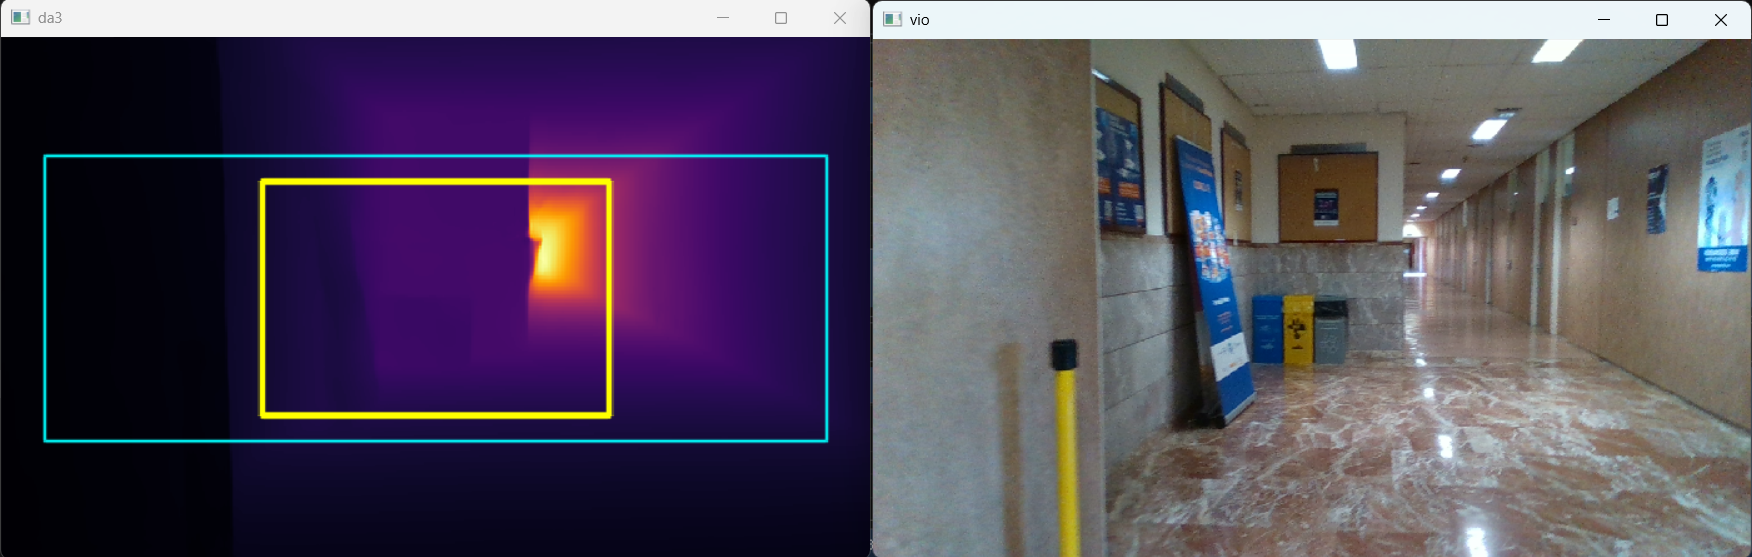
\includegraphics[width=1\textwidth]{images/roi_examp.png}
    \caption{ROI frontal en amarillo y ROI de guiado en azul. Fuente: Elaboración propia}
    \label{fig:roi_ex}
\end{figure}

\subsection{Máscara de ocupación frontal}
Dentro de la ROI frontal se umbraliza el mapa de cercanía para obtener una máscara binaria de obstáculo (\(M_F\)),~Figura \ref{fig:mask_obj}, obteniendo 1 en el caso 
de que el valor del píxel en \(C(ROI_F)\) sea mayor a un umbral de cercanía y 0 en otro caso. A partir de esta 
máscara y de la profundidad frontal se calculan las siguientes métricas:


\begin{figure}[H]
    \centering
    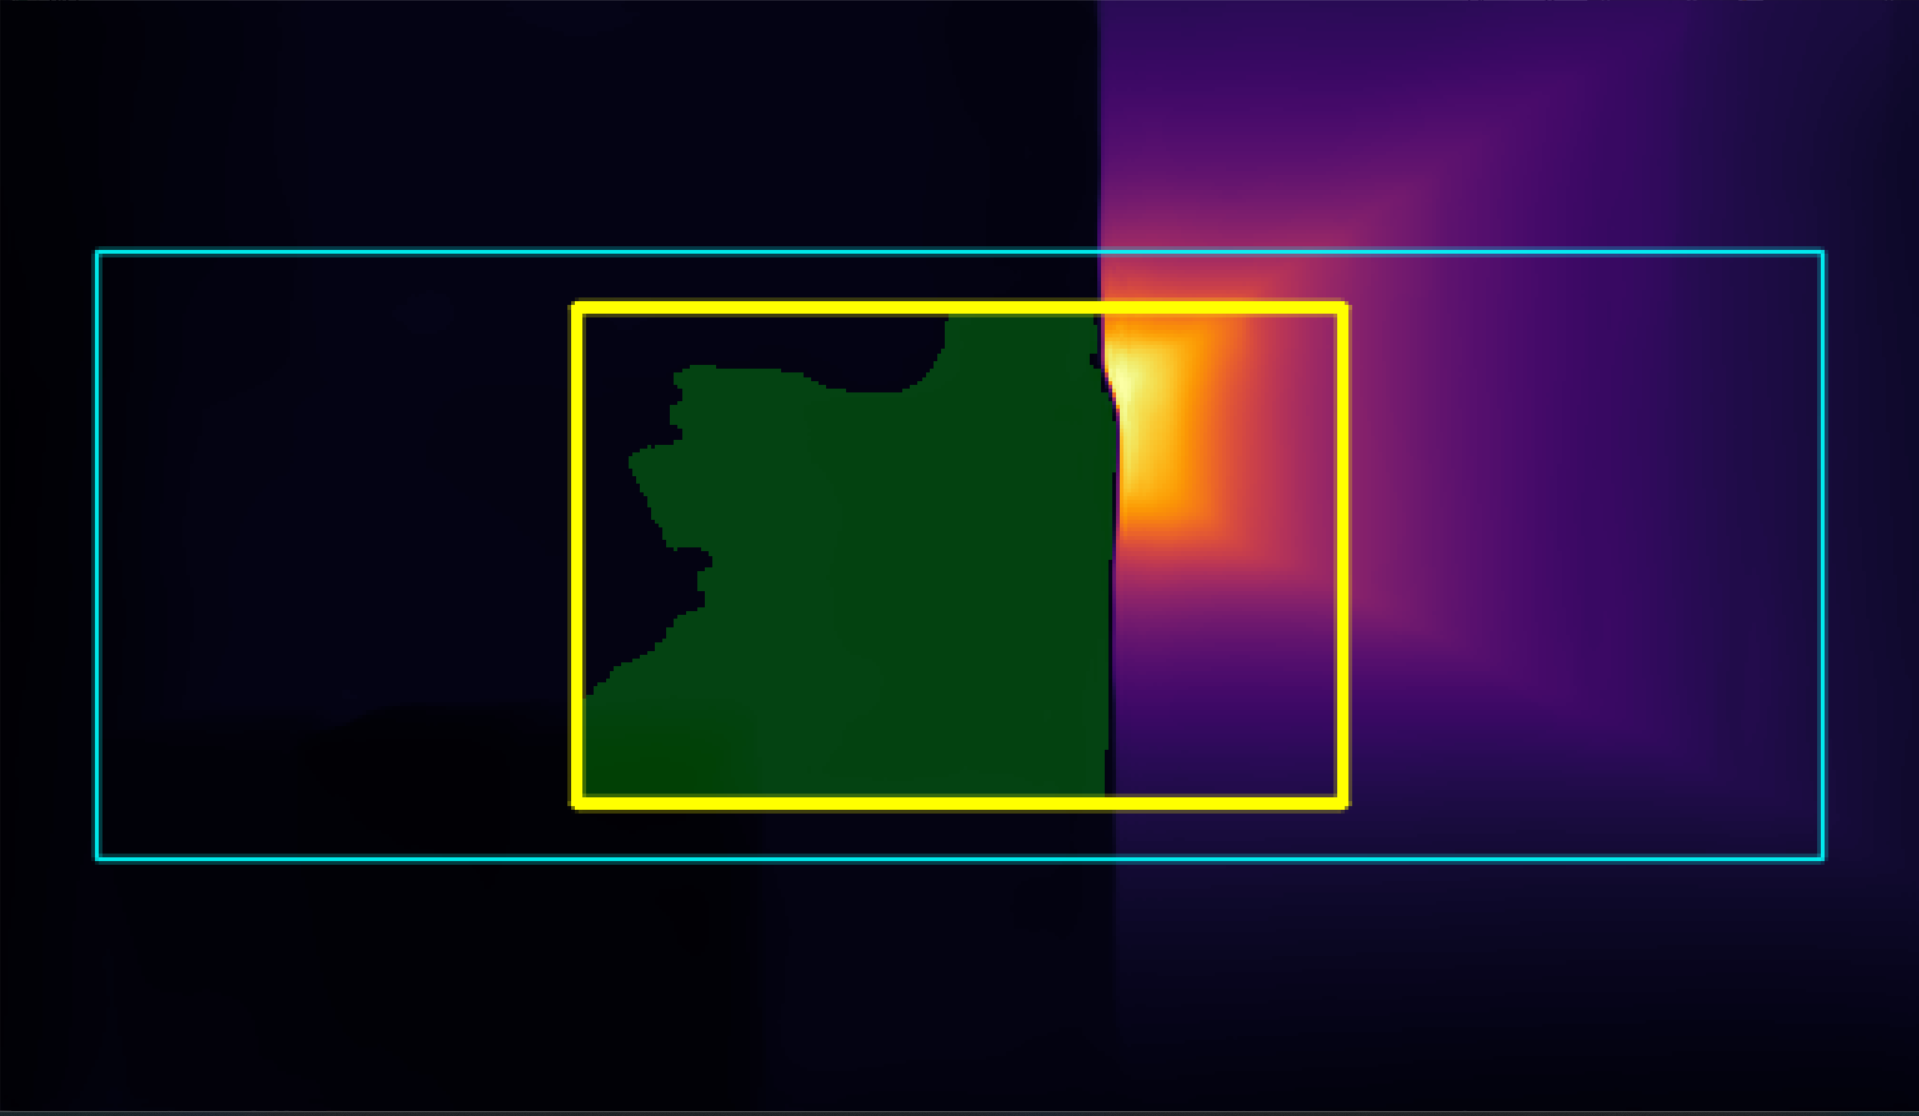
\includegraphics[width=1\textwidth]{images/mask_obj.png}
    \caption{Máscara \(M_F\) de la ROI frontal en verde. Fuente: Elaboración propia}
    \label{fig:mask_obj}
\end{figure}

\begin{itemize}
\item \textbf{Cercanía media frontal:} \(\bar{C}_F = \frac{1}{N_F}\sum C(ROI_F)\)

\item \textbf{Área ocupada:} \(A_F = \frac{1}{N_F}\sum M_F(ROI_F)\)

\item \textbf{Ratio de mayor área conexa:}\(B_F = \frac{\text{Mayor área conexa en } M_F}{N_F}\)

\item \textbf{Profundidad frontal percentil 20:} \(d_{20} = P_{20}(D_v \text{ en } ROI_F),\)

\item \textbf{Profundidad frontal pico:} \(d_{p} = P_{q}(D_v \text{ en } ROI_F)\)
donde \(q\) es un percentil pequeño, típicamente \(q=5\), para detectar obstáculos pequeños pero muy cercanos.
\end{itemize}

Estas dos últimas profundidades se convierten también a cercanía normalizada:

\[
c_{20} = \mathrm{clip}\!\left(1-\frac{d_{20}-p_{10}}{p_{90}-p_{10}},\,0,\,1\right),
\qquad
c_{p} = \mathrm{clip}\!\left(1-\frac{d_{p}-p_{10}}{p_{90}-p_{10}},\,0,\,1\right).
\]


\subsection{Cálculo de la puntuación de obstáculo}

Con las métricas anteriores se construye una puntuación escalar de obstáculo, esto se puede observar en la Figuras~\ref{fig:prop_noevad} y \ref{fig:prop_evad}:
\[ S_t = w_1 \bar{C}_F + w_2 A_F + w_3 B_F + w_4 c_{20} + w_5 c_p. \]


Esta puntuación se filtra temporalmente mediante un suavizado exponencial:

\begin{figure}[H]
    \centering
    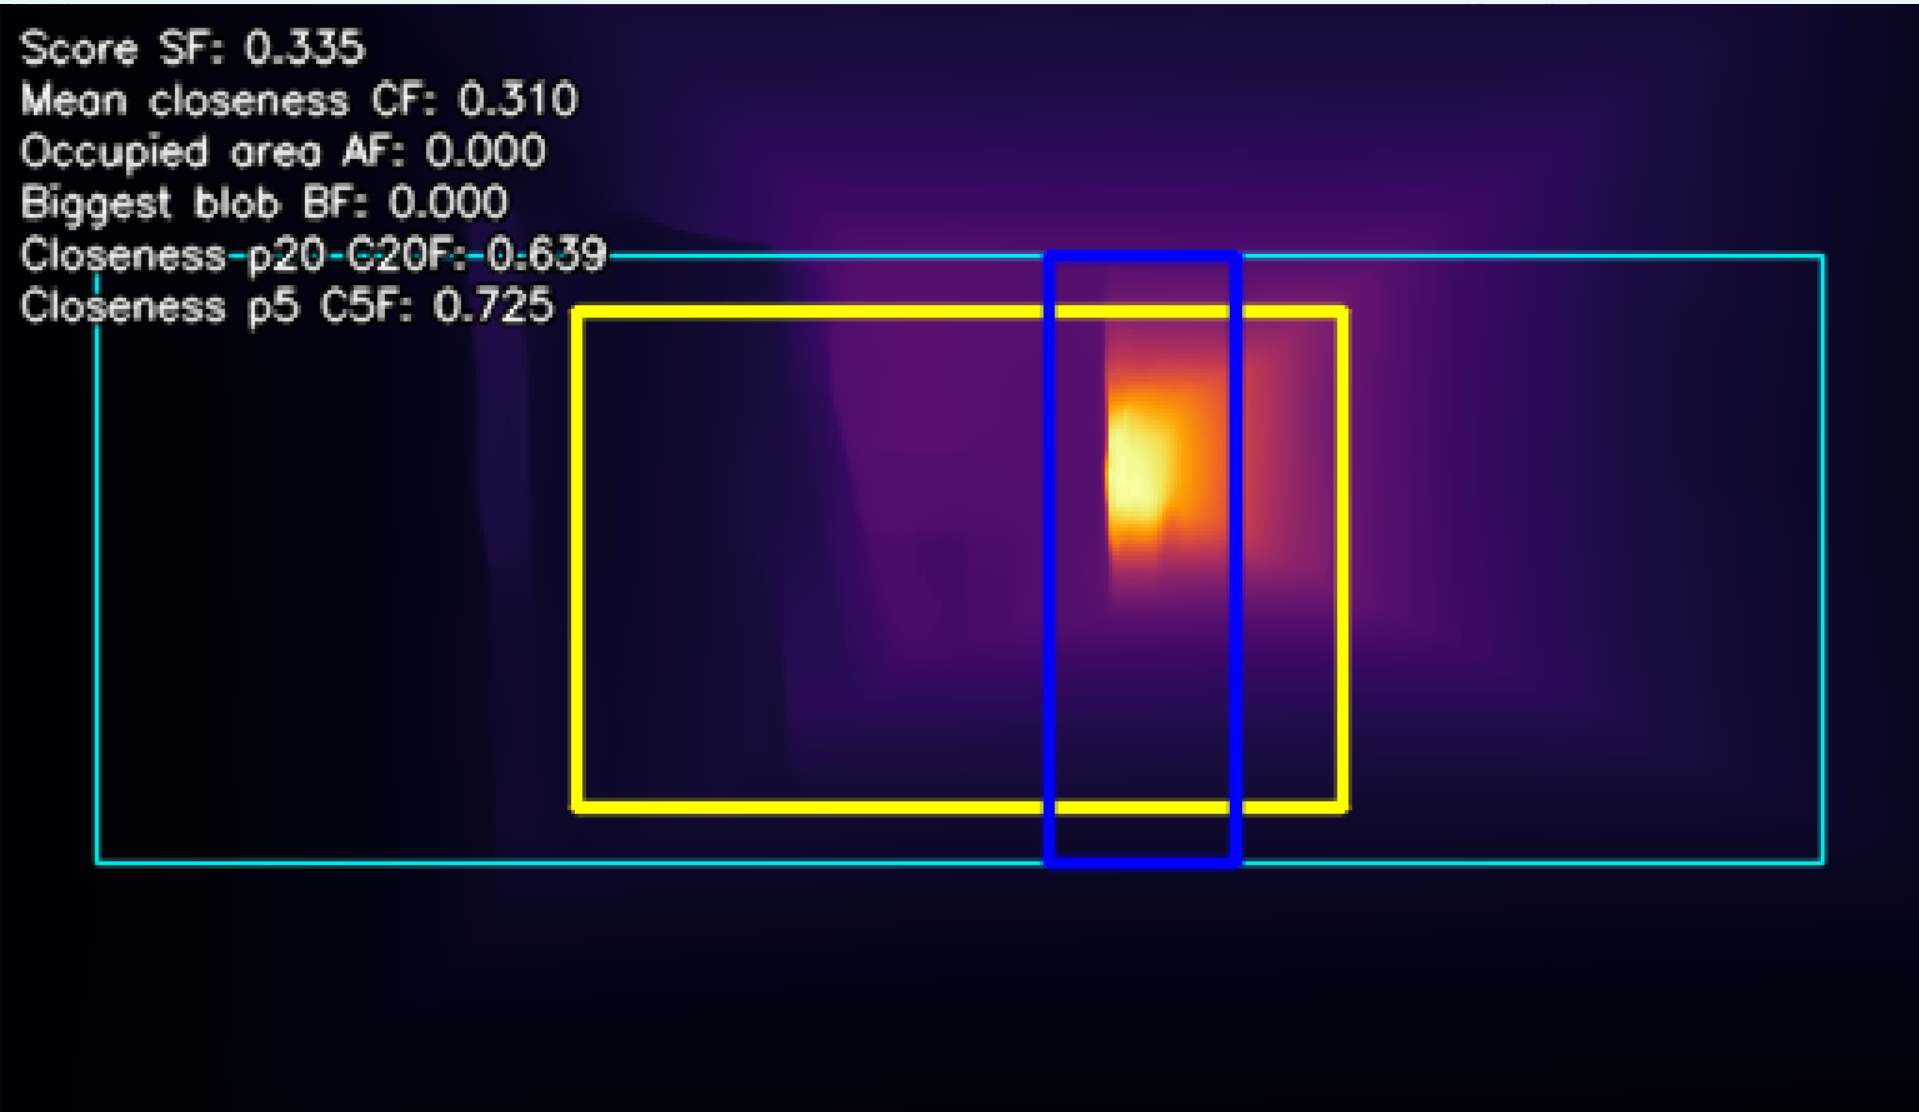
\includegraphics[width=1\textwidth]{images/prop_noevad.png}
    \caption{Ejemplo de propiedades sin obstáculo presente. Fuente: Elaboración propia}
    \label{fig:prop_noevad}
\end{figure}

\begin{figure}[H]
    \centering
    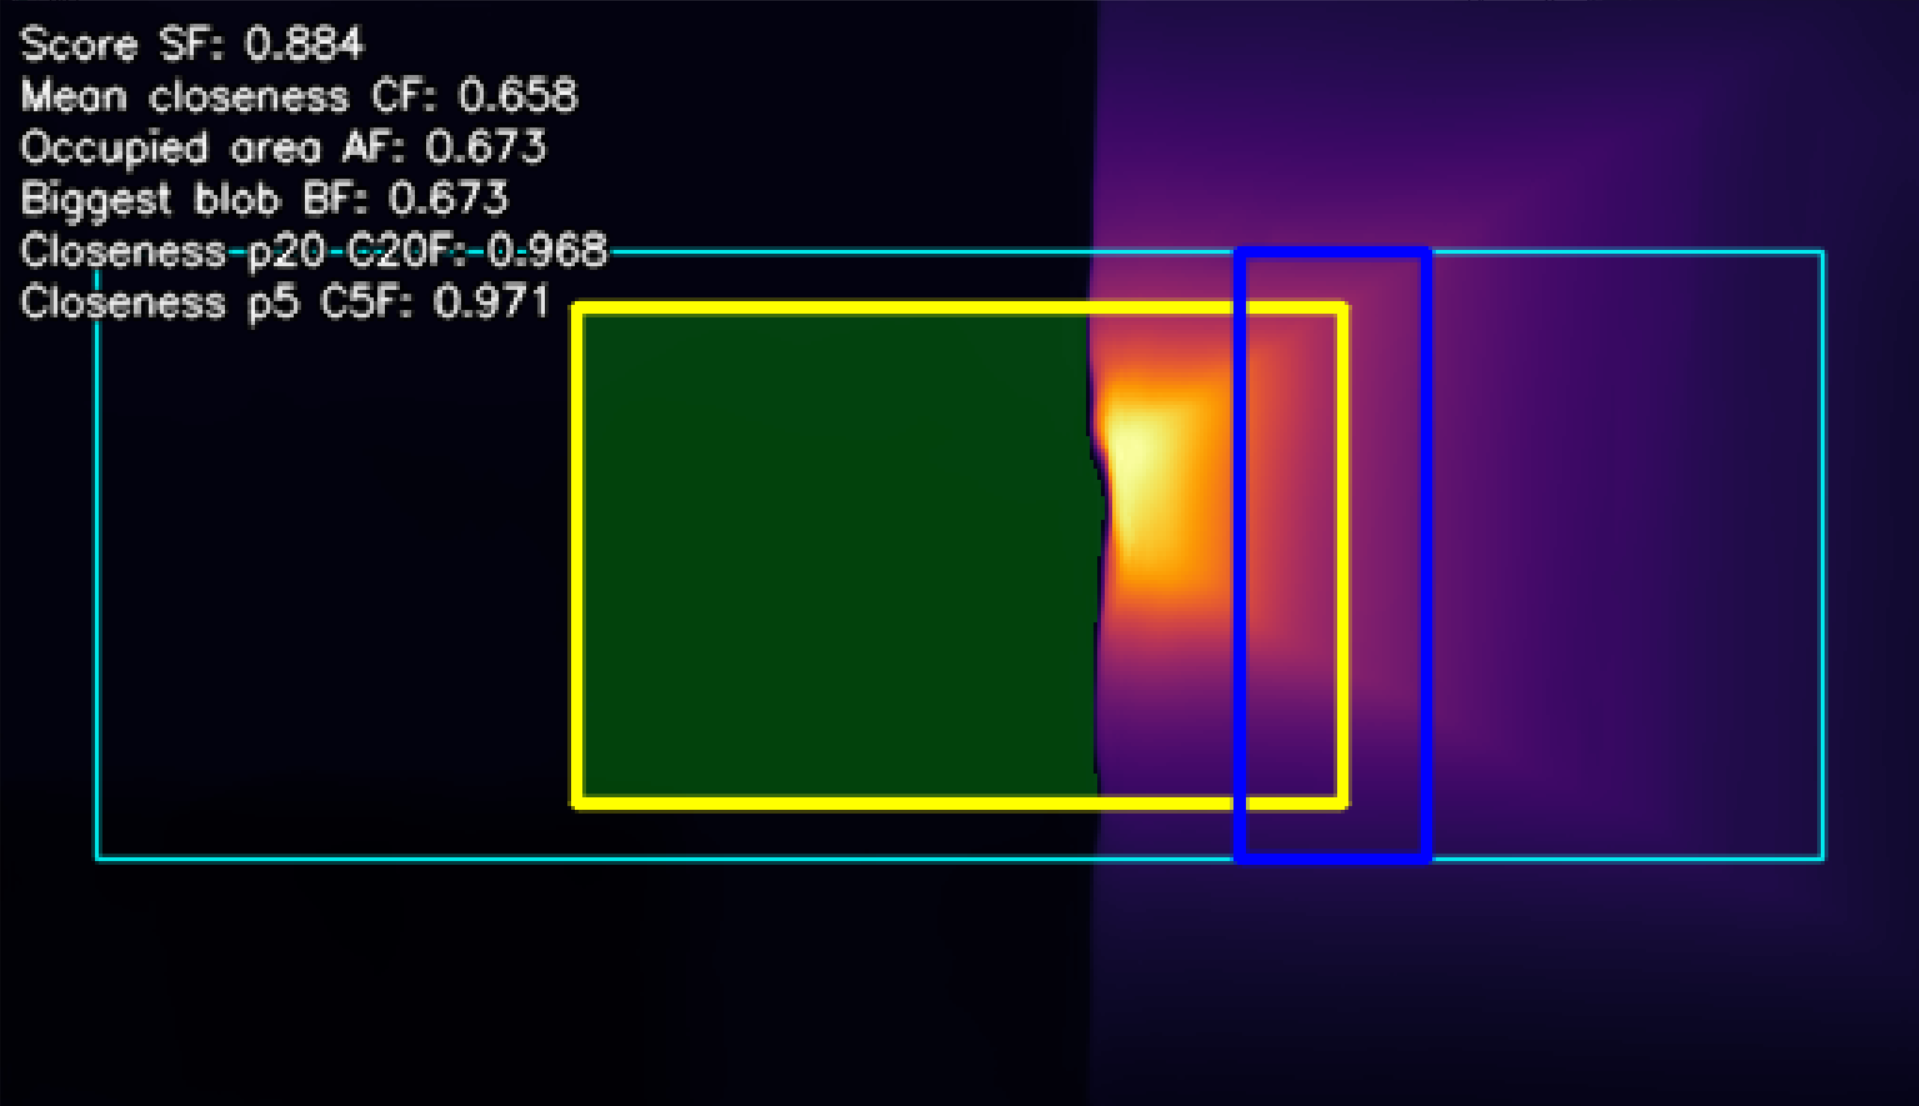
\includegraphics[width=1\textwidth]{images/prop_evad.png}
    \caption{Ejemplo de propiedades con obstáculo presente. Fuente: Elaboración propia}
    \label{fig:prop_evad}
\end{figure}


\[
\tilde{S}_t = \alpha_S \tilde{S}_{t-1} + (1-\alpha_S)S_t
\]
donde \(\alpha_S \in [0,1]\) es el factor de suavizado de la puntuación y \(\tilde{S}_t\) representa la puntuación filtrada.

\subsection{Activación del aviso de evitación}

La bandera binaria de evitación \(must\_evade\) indica si el módulo considera necesario avisar al planificador local de la 
presencia de un obstáculo frontal. Esta variable no se obtiene directamente del modelo de profundidad, sino a partir 
de una combinación de condiciones sobre la profundidad estimada, la ocupación de la región frontal y la puntuación global 
de obstáculo.

Para ello se definen varios umbrales:
\begin{itemize}
    \item El umbral \(d_{\text{evade}}\) representa un umbral operativo aplicado sobre la profundidad frontal estimada por el modelo para decidir si un obstáculo se considera relevante para la evasión. Aunque su valor se expresa en las mismas unidades manejadas por la salida del modelo, en este trabajo su uso debe interpretarse como un criterio práctico de activación dentro de la cadena completa de decisión, no como una medida física absoluta suficiente por sí sola. 
    \item El umbral \(T_p\) define el valor mínimo de cercanía pico (percentil 5\%) necesario para considerar que existe 
    una zona especialmente próxima al vehículo. 
    \item Los umbrales \(A_{\min}\) y \(B_{\min}\) establecen, respectivamente, el porcentaje mínimo de área cercana y el 
    tamaño mínimo del mayor obstáculo conexo dentro de la región frontal. 
    \item El umbral \(T_{\text{on}}\) es el umbral de activación de la puntuación global de obstáculo.
    \item El umbral \(T_{\text{off}}\) es el umbral de desactivación empleado para introducir histéresis.
\end{itemize}
Las condiciones de activación son las siguientes:

\begin{itemize}
    \item activación por profundidad frontal, cuando el percentil 20 de profundidad en la región frontal es menor o igual que el umbral operativo de evasión:
    \[d_{20} \le d_{\text{evade}}\]

    \item activación por cercanía pico, cuando la zona más próxima de la región frontal supera el umbral de cercanía definido:
    \[c_p \ge T_p\]

    \item activación por ocupación, cuando el área cercana o el mayor obstáculo conexo dentro de la región frontal superan sus respectivos umbrales:
    \[A_F \ge A_{\min} \quad \text{o} \quad B_F \ge B_{\min}\]

    \item activación por puntuación global, cuando la puntuación de obstáculo filtrada supera el umbral de activación:
    \[\tilde{S}_t \ge T_{\text{on}}\]
\end{itemize}

Estas condiciones se combinan en una única señal lógica de activación, denotada por \(\mathrm{threshold\_hit}_t\), de manera que sea suficiente el cumplimiento de una de ellas
para la activación de la bandera booleana:

\[
\mathrm{threshold\_hit}_t =
(d_{20} \le d_{\text{evade}}) || (c_p \ge T_p) || (A_F \ge A_{\min}) || (B_F \ge B_{\min}) || (\tilde{S}_t \ge T_{\text{on}}). \]

Una vez activado el aviso de evitación, la desactivación no se realiza con el mismo umbral de activación, sino con un umbral inferior \(T_{\text{off}}\). De este modo, si el sistema ya estaba en estado de evasión, la bandera se mantiene activa mientras la puntuación de obstáculo siga siendo suficientemente alta:

\[
\tilde{S}_t \ge T_{\text{off}}.
\]

Por tanto, la actualización final de la bandera de evitación queda definida como:

\[
\mathrm{must\_evade}_t =
\begin{cases}
1, & \text{si } \mathrm{must\_evade}_{t-1}=0 \text{ y } \mathrm{threshold\_hit}_t,\\
1, & \text{si } \mathrm{must\_evade}_{t-1}=1 \text{ y } \tilde{S}_t \ge T_{\text{off}},\\
0, & \text{en otro caso.}
\end{cases}
\]

Este comportamiento introduce una histéresis en la activación del aviso. El sistema se activa cuando 
alguna condición supera su umbral correspondiente, pero solo se desactiva cuando la puntuación global cae por debajo de 
\(T_{\text{off}}\). Al ser \(T_{\text{off}}\) menor que \(T_{\text{on}}\), se evita que la bandera \(must\_evade\) conmute 
rápidamente entre activa e inactiva cuando la escena se encuentra cerca del límite de decisión. Todo este comportamiento 
se puede comprobar en las Figuras~\ref{fig:mustevade_false} y \ref{fig:mustevade_true}.



\begin{figure}[H]
    \centering
    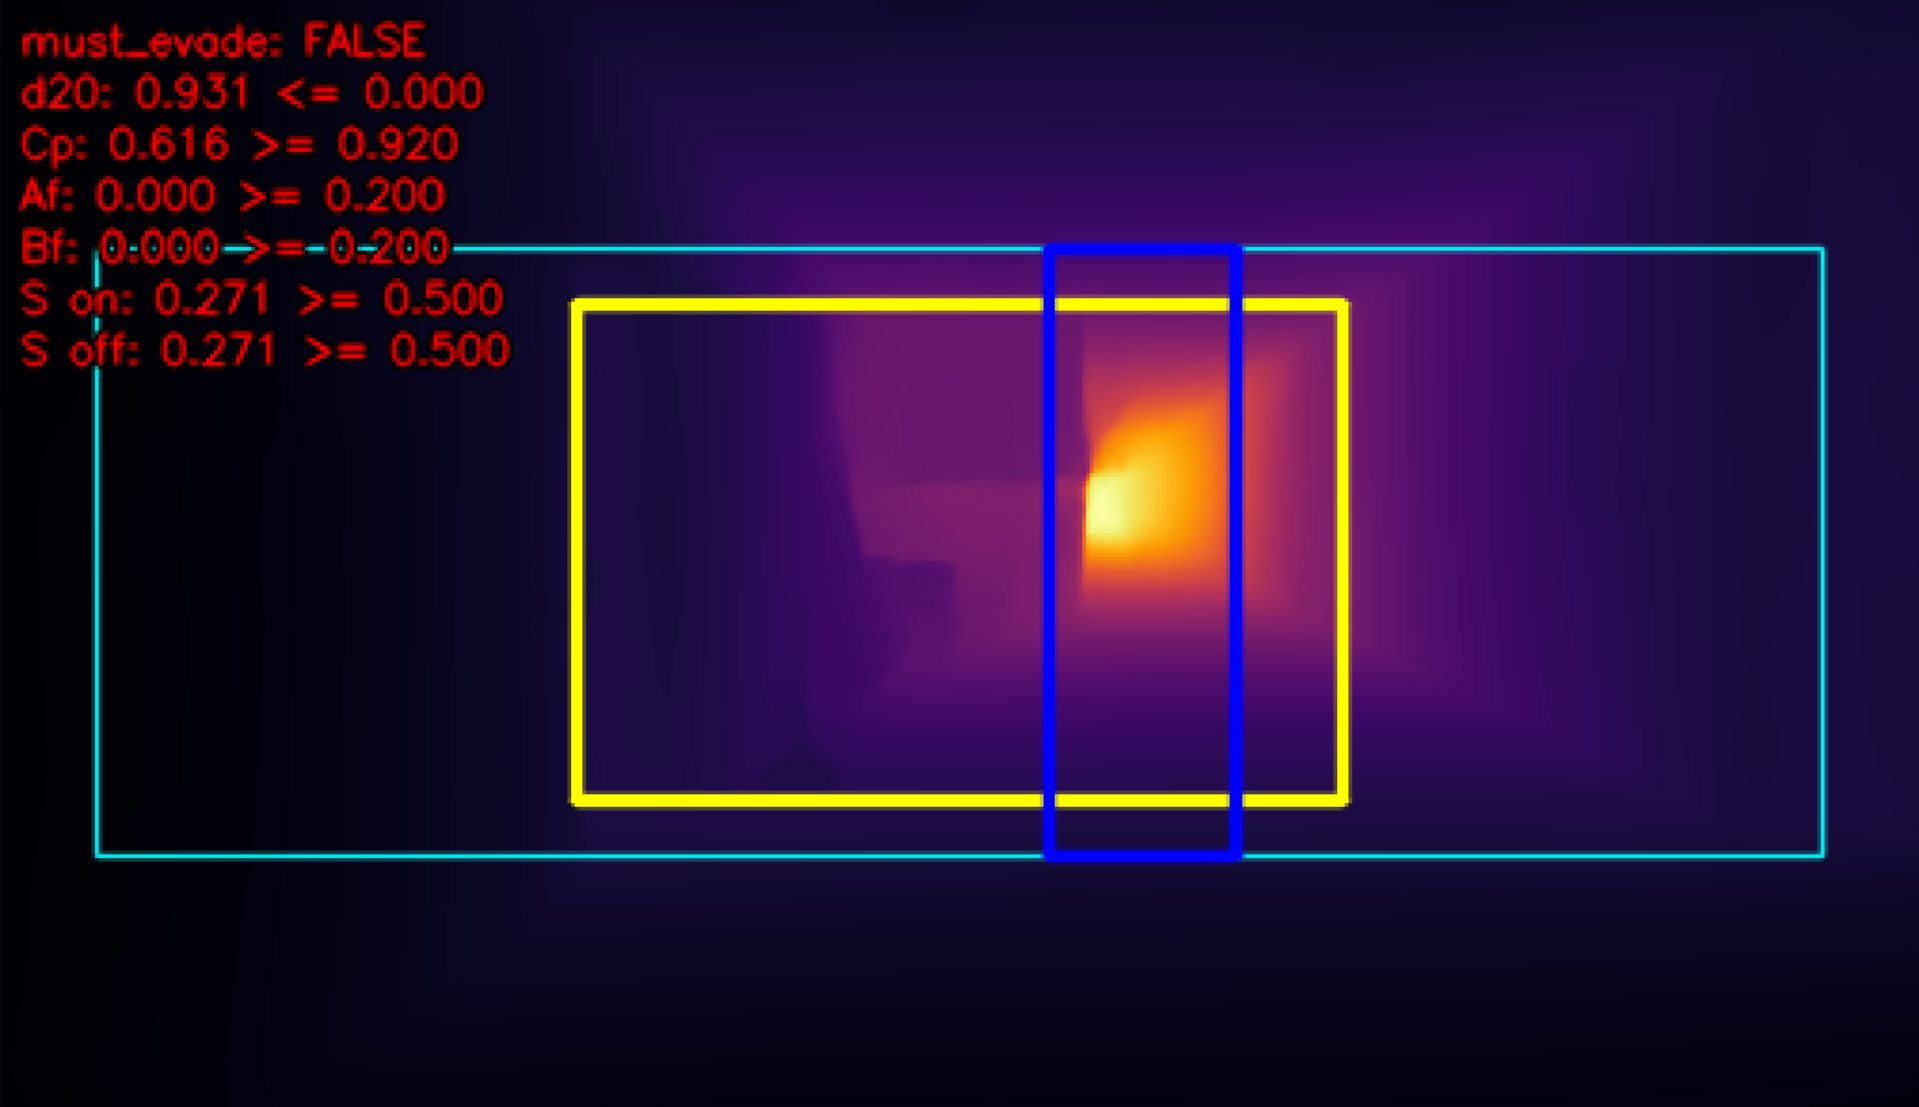
\includegraphics[width=1\textwidth]{images/mustevade_false.png}
    \caption{Ejemplo de condiciones no cumplidas. Fuente: Elaboración propia}
    \label{fig:mustevade_false}
\end{figure}

\begin{figure}[H]
    \centering
    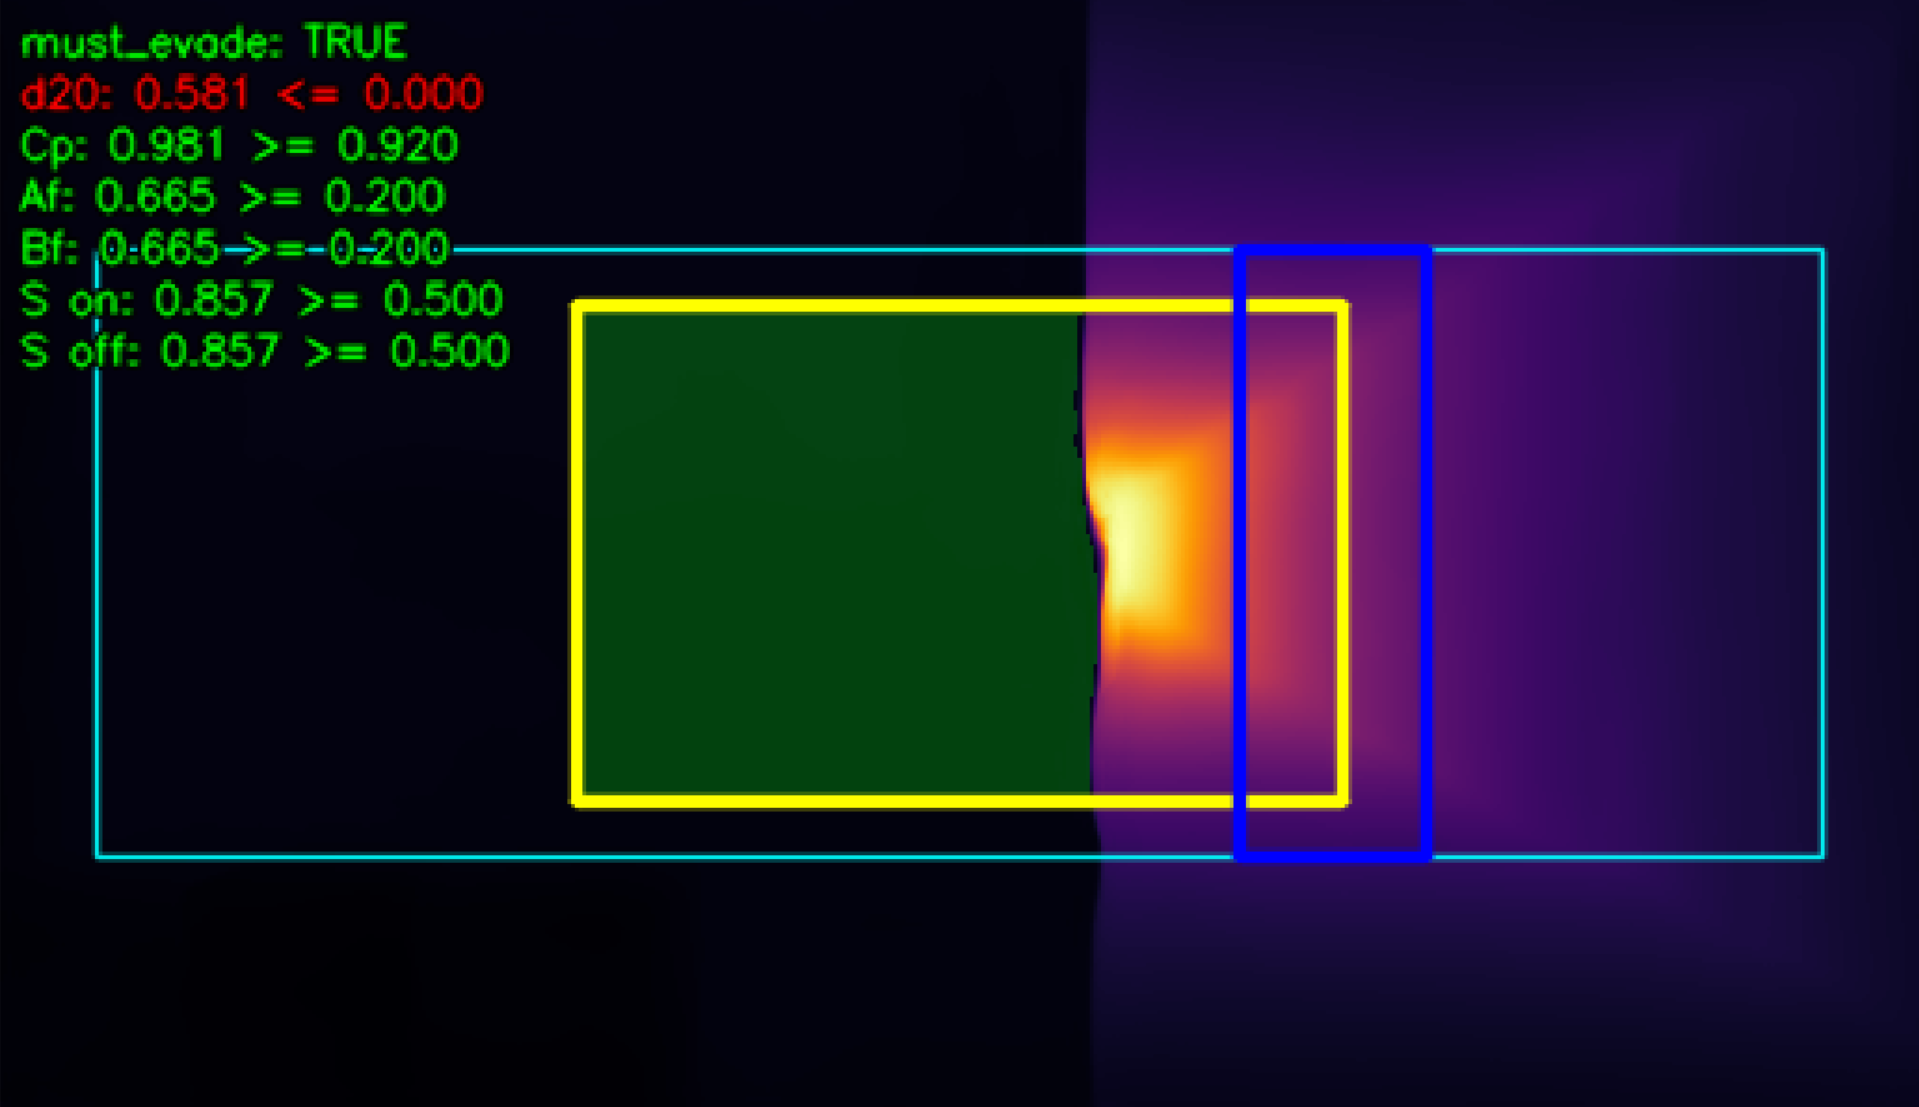
\includegraphics[width=1\textwidth]{images/mustevade_true.png}
    \caption{Ejemplo de condiciones cumplidas. Fuente: Elaboración propia}
    \label{fig:mustevade_true}
\end{figure}


\subsection{Cálculo de la dirección de evitación}

La dirección de evitación se calcula identificando hacia qué zona de la imagen conviene desplazar la referencia lateral 
de evasión. Para ello, se utiliza la ROI de guiado, que corresponde a una región amplia de la imagen centrada en la zona 
de avance del UAV. Esta región se divide en varios sectores verticales, de forma que cada uno de ellos representa una 
posible dirección lateral de escape como se puede ver en la Figura~\ref{fig:sectors}.


\begin{figure}[H]
    \centering
    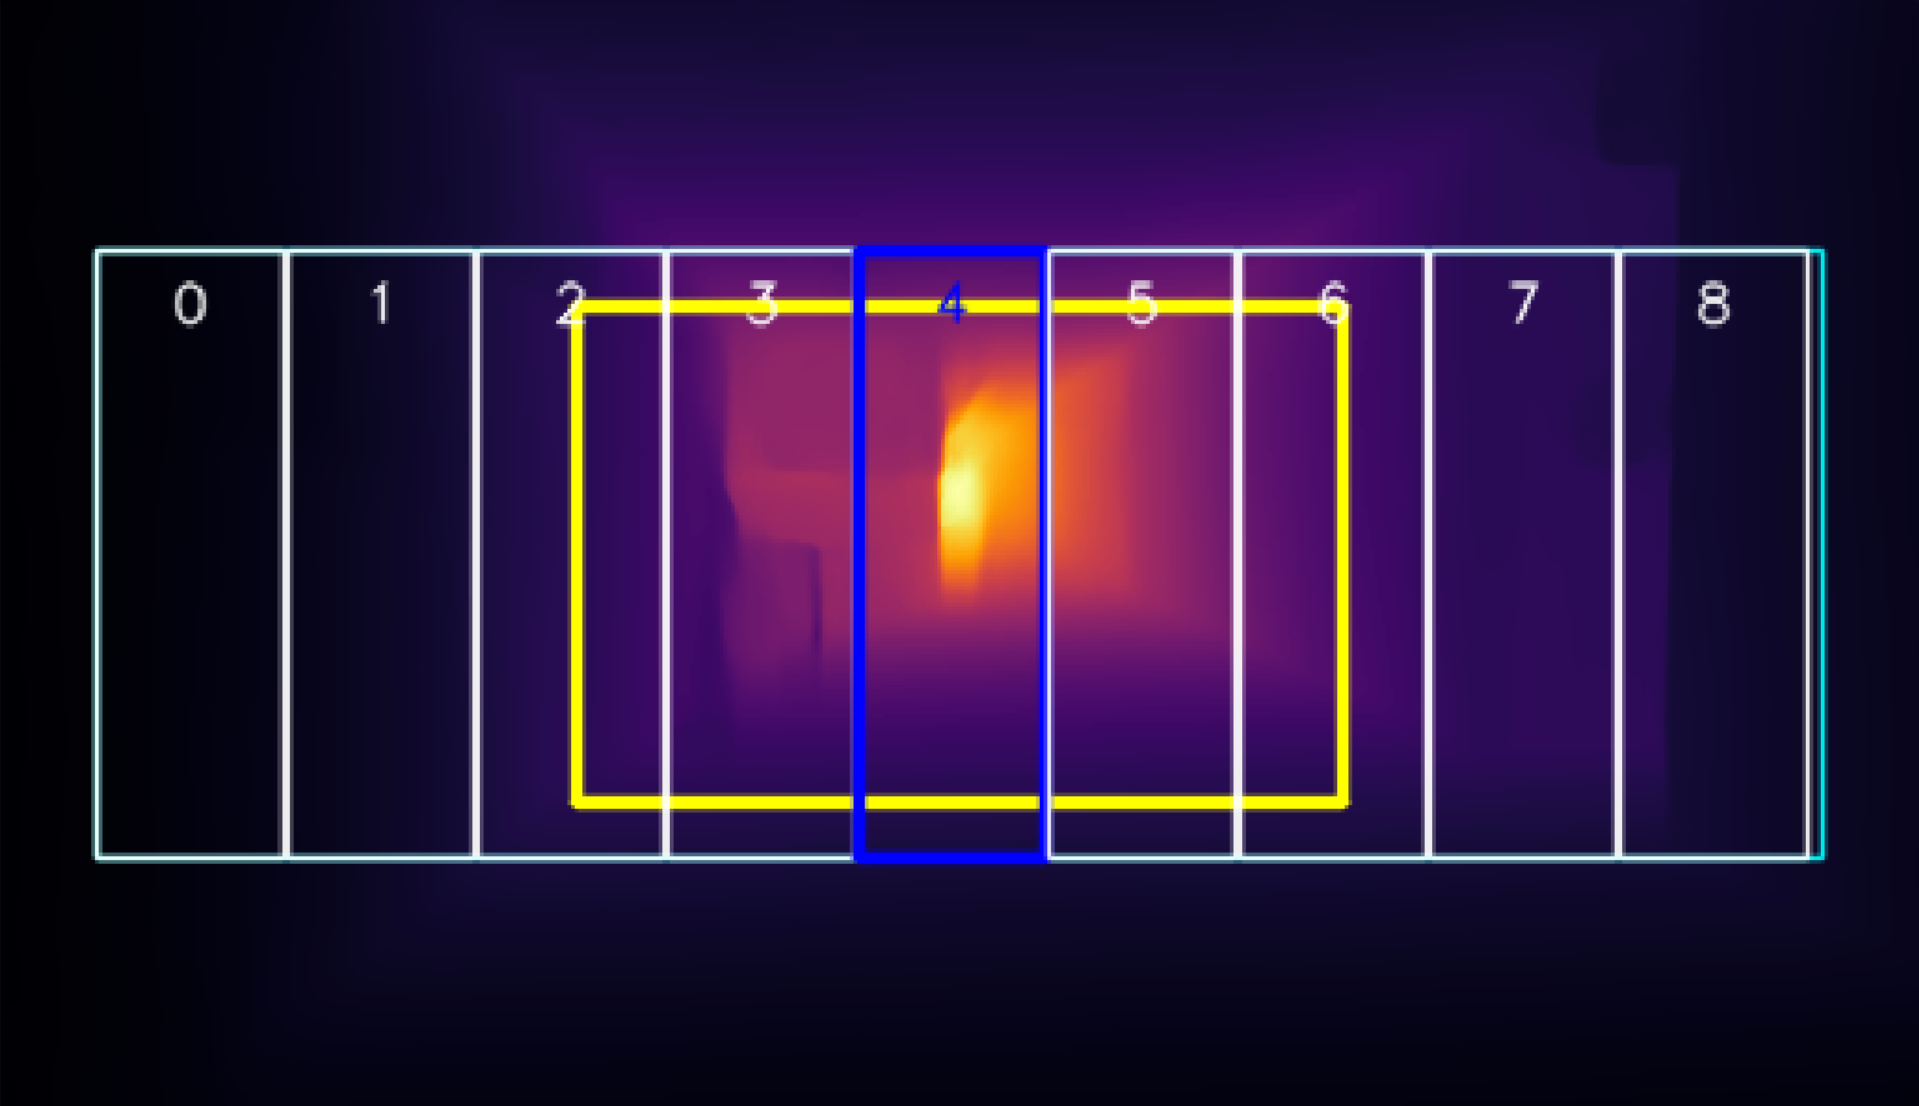
\includegraphics[width=1\textwidth]{images/sectors_ex.png}
    \caption{ROI de guiado dividida en 9 sectores verticales, en azul el sector seleccionado. Fuente: Elaboración propia}
    \label{fig:sectors}
\end{figure}

En cada sector se evalúan dos aspectos principales. En primer lugar, se calcula la profundidad normalizada media, que 
indica si esa zona de la imagen corresponde, en promedio, a una región lejana. Un valor alto indica que el sector 
corresponde, en promedio, a una zona relativamente más despejada dentro de la imagen. En segundo lugar, se calcula la 
proporción de píxeles cercanos, es decir, 
aquellos cuya cercanía supera el umbral definido para detectar ocupación próxima.

A partir de estas dos magnitudes se asigna una puntuación de espacio libre a cada sector:

\[
g_i = \overline{D}_{n,i} - \lambda \rho_i,
\]

donde \(\overline{D}_{n,i}\) es la profundidad normalizada media del sector \(i\), \(\rho_i\) es la proporción de píxeles 
cercanos dentro de dicho sector y \(\lambda\) es un factor de penalización. Esta penalización permite descartar sectores 
que, aunque puedan parecer relativamente profundos en promedio, contienen una cantidad significativa de píxeles cercanos 
y, por tanto, no son adecuados como dirección de evasión.

Una vez calculada la puntuación de todos los sectores, se selecciona aquel que presenta el mayor valor:

\[
i^\star = \arg\max_i g_i.
\]

El sector \(i^\star\) se interpreta como la dirección lateral preferente dentro de la ROI de guiado según la puntuación 
definida. Sin embargo, no se toma simplemente el centro geométrico del sector como punto objetivo, sino que se calcula un 
centroide ponderado hacia las zonas más lejanas. Para ello, cada píxel del sector recibe un peso proporcional a su 
profundidad normalizada, elevando el peso al cuadrado, de manera que los píxeles correspondientes a regiones lejanas 
tengan más influencia en el cálculo del punto objetivo que aquellos situados en zonas menos despejadas.

\[
w(x,y)=D_n(x,y)^2.
\]

El punto objetivo dentro del sector seleccionado se calcula como:

\[
\mathbf{p}^\star =
\frac{\sum w(x,y)\,[x\;\;y]^T}{\sum w(x,y)}.
\]

De esta forma, el punto \(\mathbf{p}^\star\) queda desplazado hacia la zona más libre del mejor sector. Si no existe 
suficiente información válida para calcular este centroide ponderado, se utiliza como alternativa el centro geométrico 
del sector seleccionado.

A continuación, se calcula un vector desde el centro de la imagen hasta el punto objetivo:

\[
\mathbf{u} = \mathbf{p}^\star - \mathbf{p}_c,
\]

donde \(\mathbf{p}_c\) representa el centro de la imagen. Este vector indica hacia qué zona de la imagen debería 
desplazarse el UAV para evitar el obstáculo. En coordenadas de imagen, una componente horizontal positiva indica una 
dirección hacia la derecha, mientras que una componente horizontal negativa indica una dirección hacia la izquierda.

Para evitar cambios bruscos entre fotogramas consecutivos, la dirección obtenida se suaviza temporalmente mediante un filtro 
exponencial:

\[
\tilde{\mathbf{u}}_t =
\alpha_u \tilde{\mathbf{u}}_{t-1} + (1-\alpha_u)\mathbf{u}_t.
\]


Finalmente, se normaliza para obtener el vector final de evitación:

\[
\mathbf{v}_t =
\begin{cases}
\dfrac{\tilde{\mathbf{u}}_t}{\|\tilde{\mathbf{u}}_t\|}, & \text{si } \|\tilde{\mathbf{u}}_t\| > \varepsilon,\\[2mm]
\mathbf{0}, & \text{en otro caso,}
\end{cases}
\]

donde \(\varepsilon\) es un umbral pequeño positivo que evita la división por valores cercanos a cero cuando la dirección de evasión no queda suficientemente definida.

Por tanto, el vector \(\mathbf{v}_t\) representa la dirección normalizada hacia la zona más segura de la imagen, y posteriormente se convierte en un ángulo de evasión 
para devolverlo como \textit{evade\_angle}, Figura~\ref{fig:evade_angle}.

\[\textit{evade\_angle} = \mathrm{atan2}(v_y, v_x).\]



\begin{figure}[H]
    \centering
    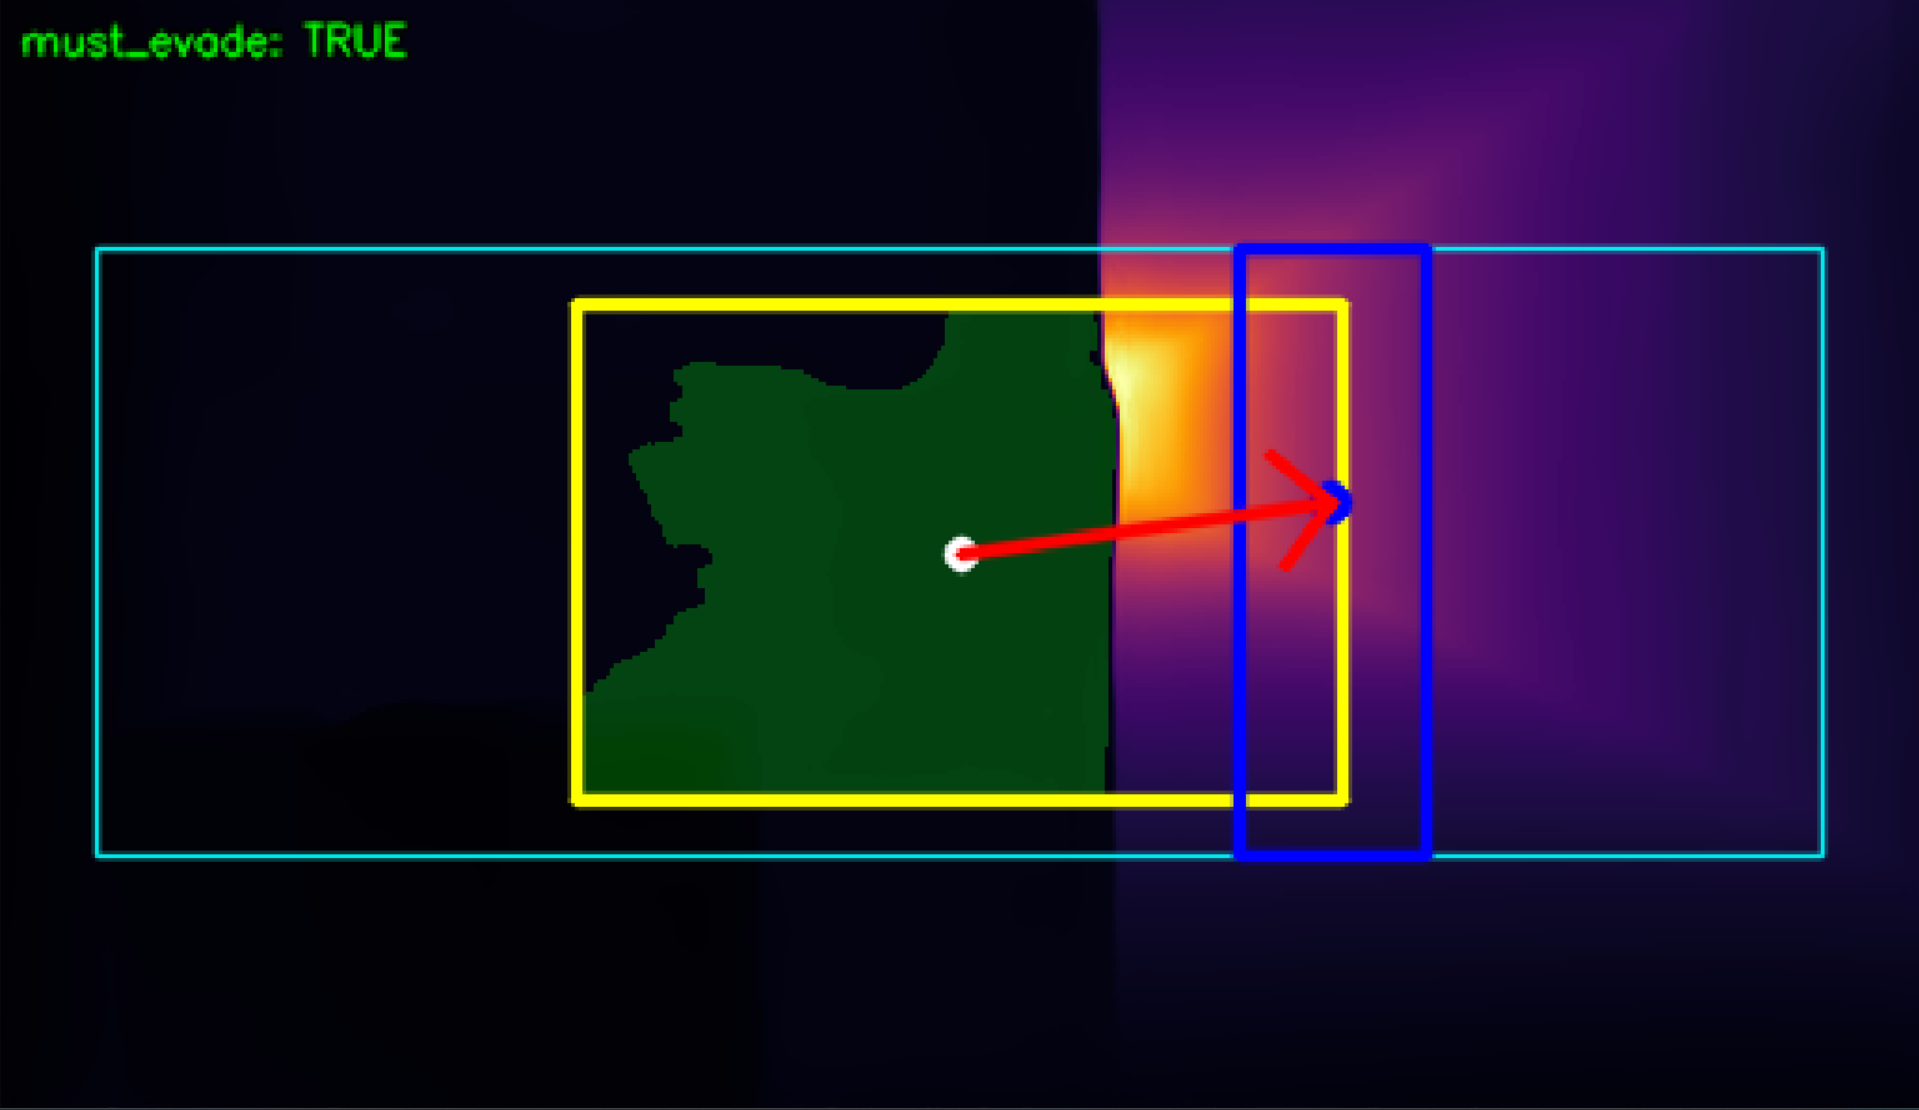
\includegraphics[width=1\textwidth]{images/evade_angle.png}
    \caption{La flecha indica la dirección de evitación decidida por el algoritmo. Fuente: Elaboración propia}
    \label{fig:evade_angle}
\end{figure}

\subsection{Interpretación}

La filosofía del algoritmo es desacoplar dos problemas distintos:

\begin{itemize}
\item \textbf{detección}: decidir si existe un obstáculo frontal suficientemente relevante como para activar evasión;
\item \textbf{guiado}: decidir hacia qué dirección conviene desplazarse una vez detectado el obstáculo.
\end{itemize}

La detección se apoya en indicadores de ocupación y cercanía frontal, mientras que la dirección se basa en la selección 
del sector con mejor puntuación de guiado. Esta separación hace al sistema más robusto que una aproximación basada 
únicamente en el gradiente medio del mapa de profundidad como se realizó en primera instancia en el proyecto de 
investigación tutelado~\cite{estudio-nav2D}.

El planificador, por tanto, recibirá las tres variables (\textit{must\_evade}, \textit{evade\_angle} y 
\textit{obstacle\_score}). En el momento en que la bandera de activación se ponga a 1, el algoritmo de planificación 
local empezará a tener en cuenta el ángulo de evitación o escape, y podrá decidir también la intensidad que debe aplicar 
a esta acción mediante la puntuación. En las siguientes gráficas de las Figuras~\ref{fig:avoidance_angle},~\ref{fig:avoidance_mag} y \ref{fig:avoidance_flag} se puede observar 
la salida de estas tres variables para un recorrido con dos obstáculos (la tercera activación de la bandera booleana corresponde al aterrizaje del dron).

\begin{figure}[H]
    \centering
    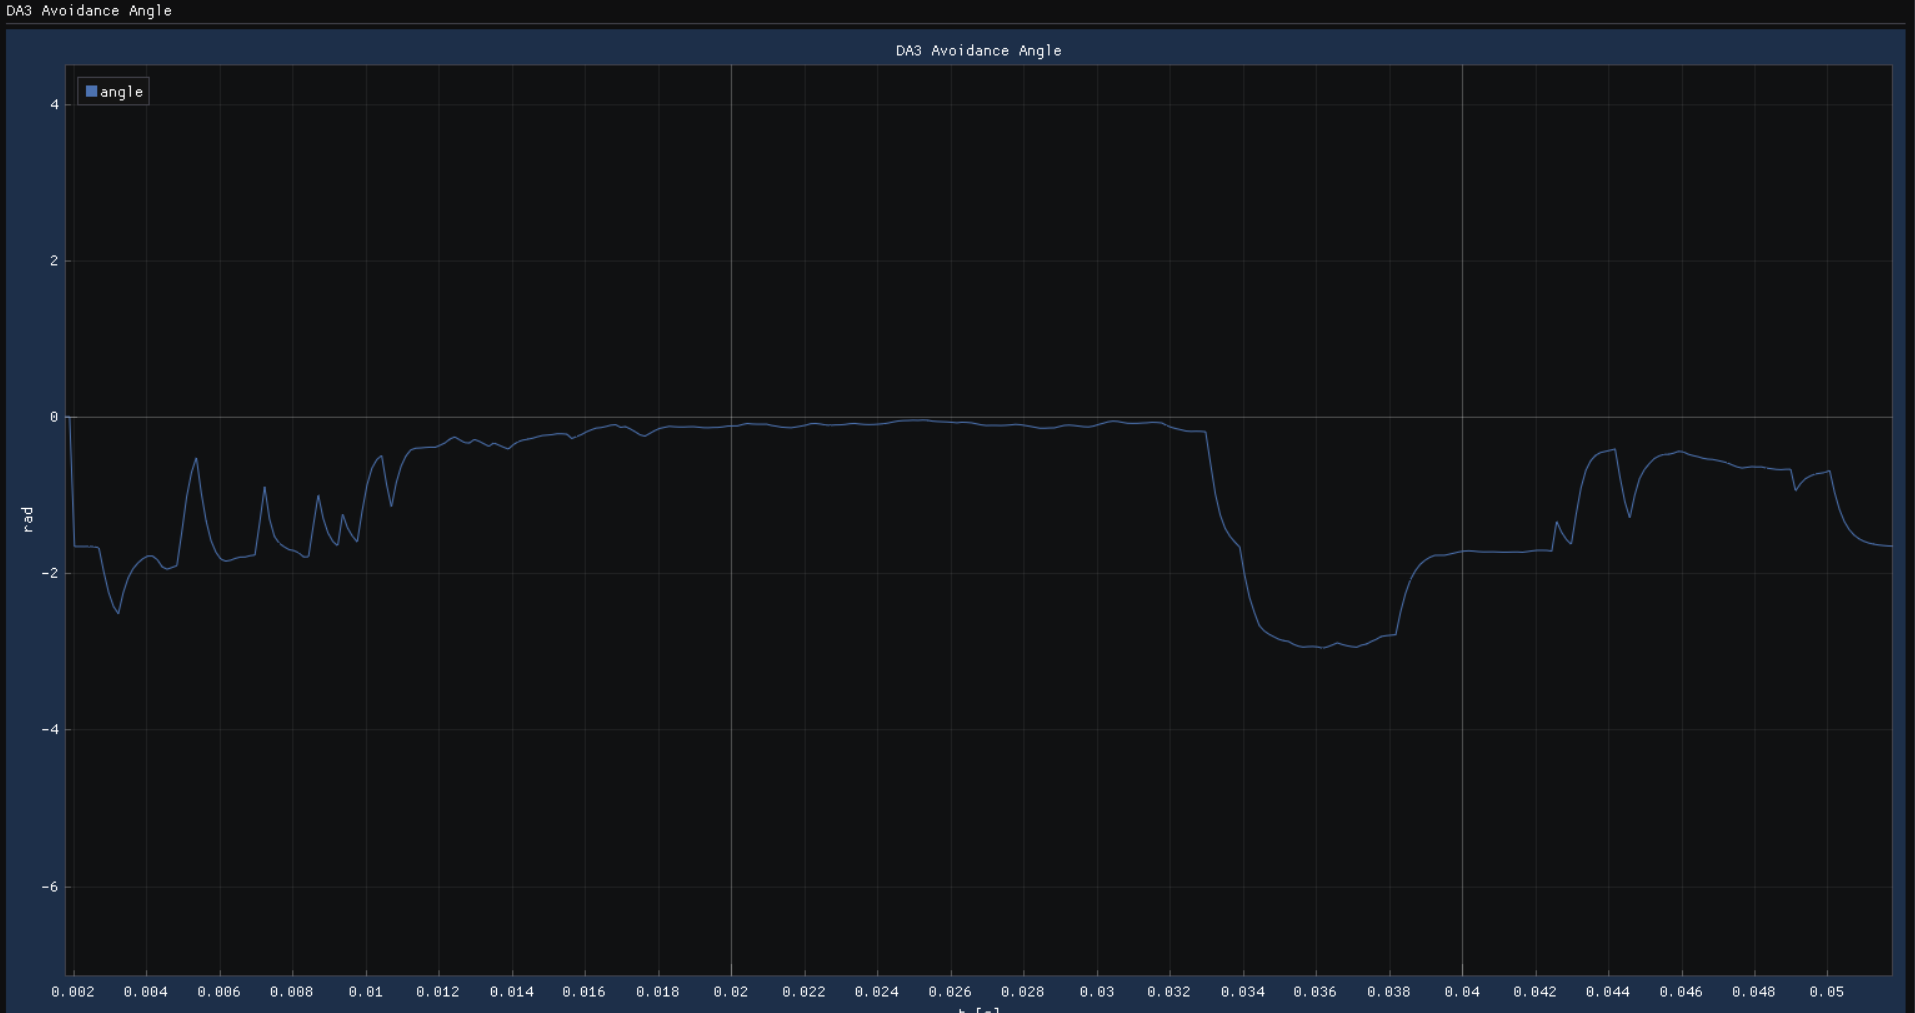
\includegraphics[width=1\textwidth]{images/avoidance_angle.png}
    \caption{Ángulo de evitación. Fuente: Elaboración propia}
    \label{fig:avoidance_angle}
\end{figure}

\begin{figure}[H]
    \centering
    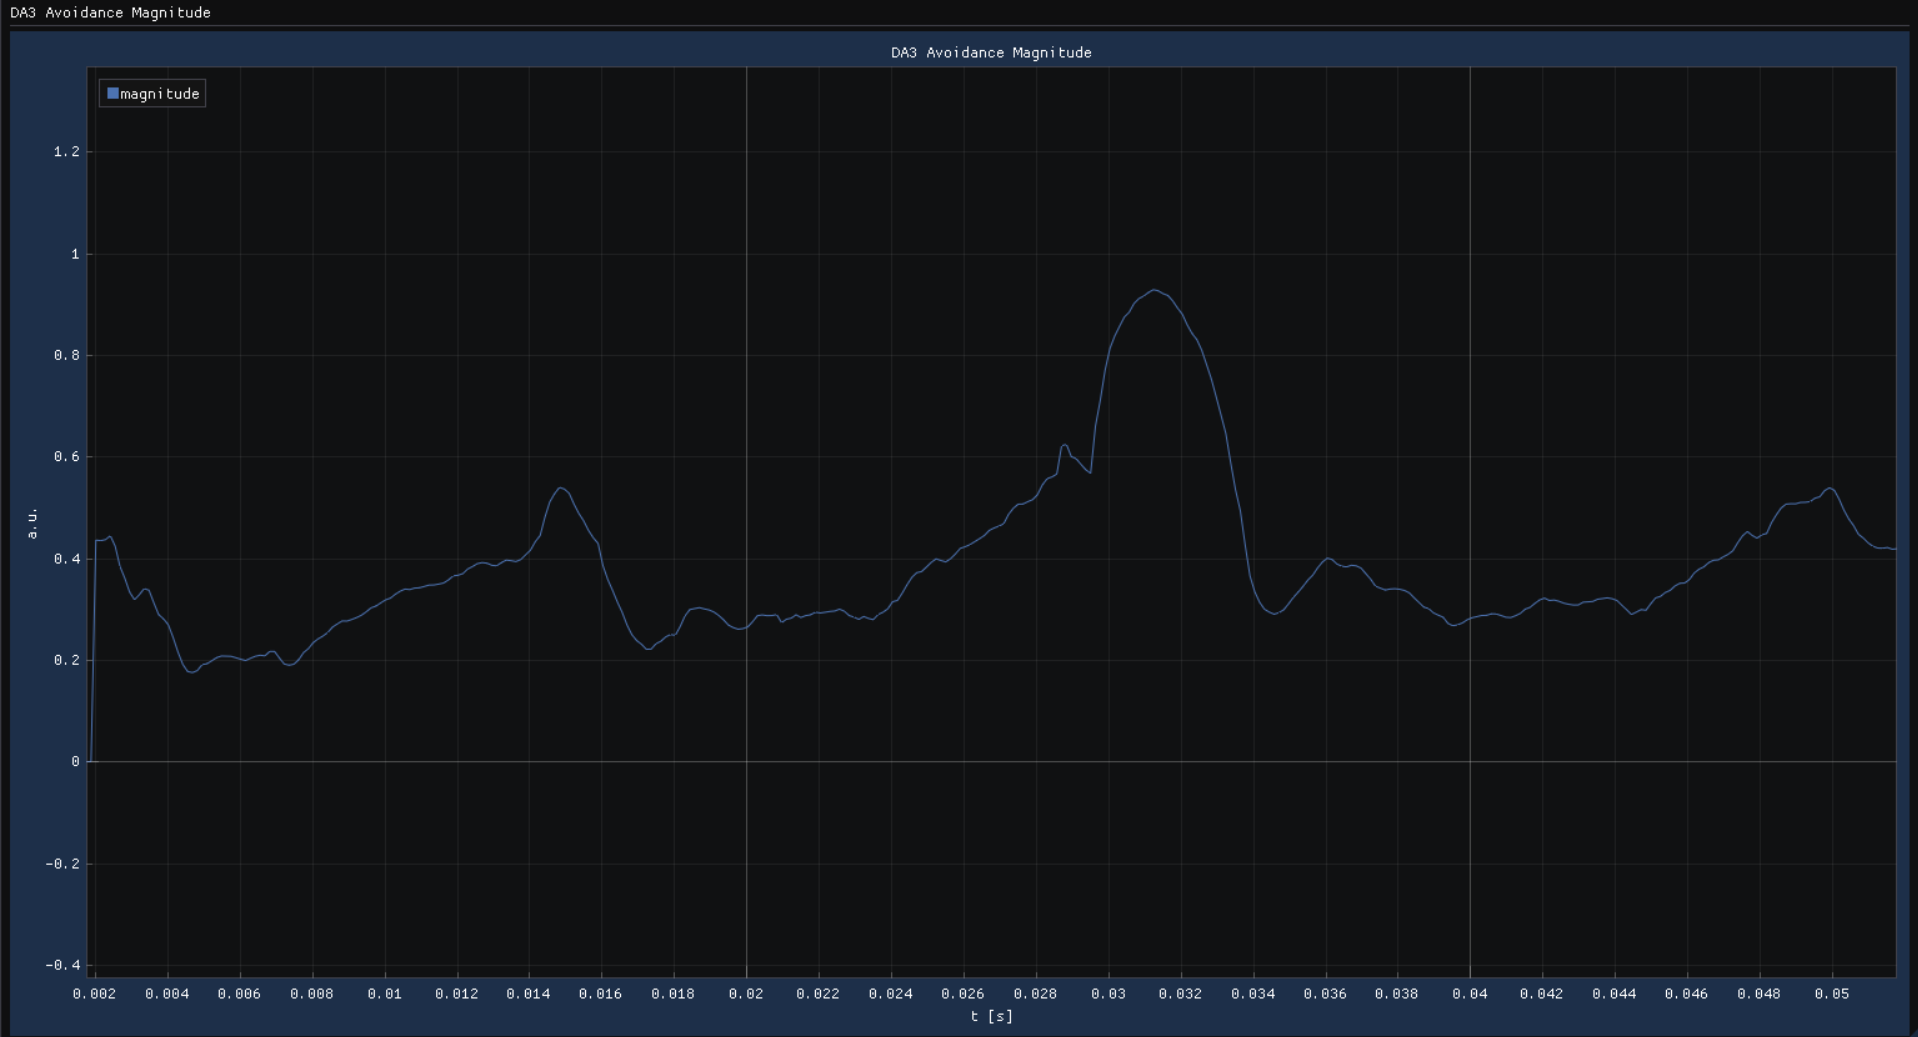
\includegraphics[width=1\textwidth]{images/avoidance_mag.png}
    \caption{Puntuación de obstáculo. Fuente: Elaboración propia}
    \label{fig:avoidance_mag}
\end{figure}
\begin{figure}[H]
    \centering
    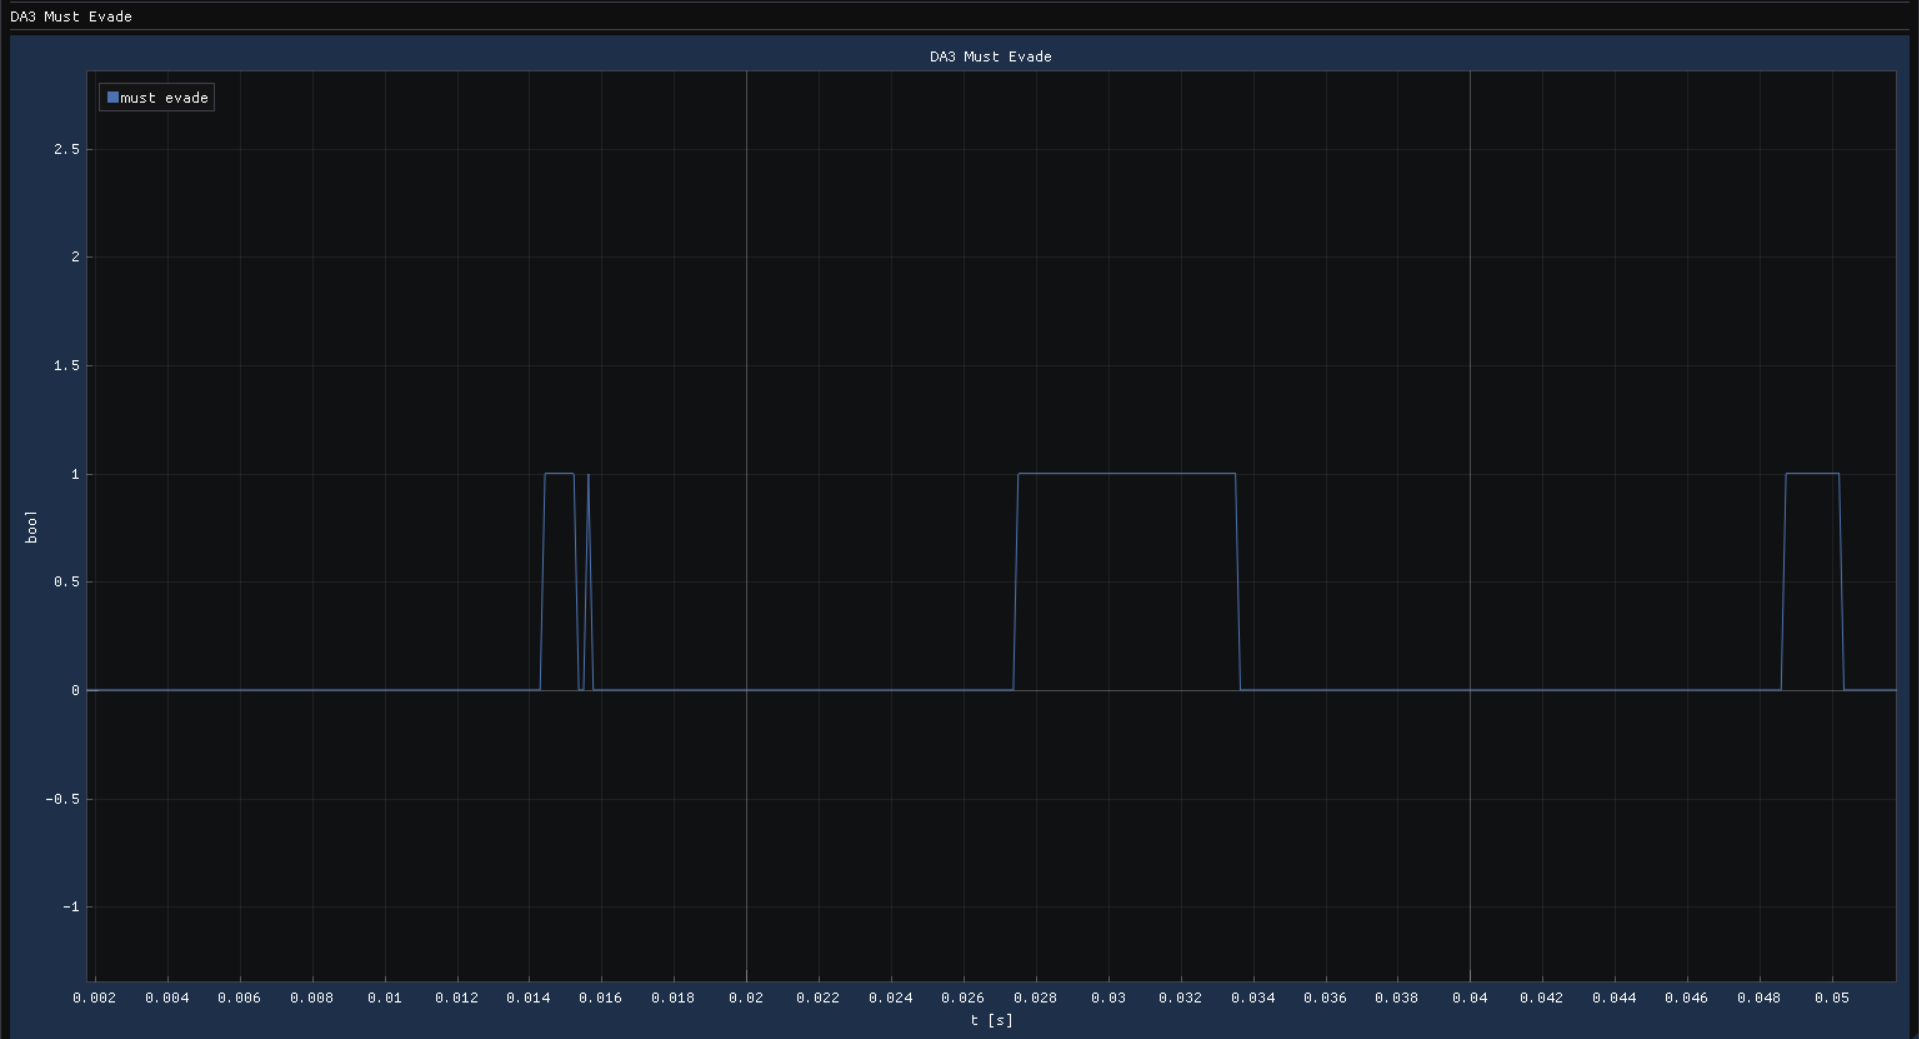
\includegraphics[width=1\textwidth]{images/avoidance_flag.png}
    \caption{Bandera de evitación booleana (1 activada, 0 desactivada). Fuente: Elaboración propia}
    \label{fig:avoidance_flag}
\end{figure}

\chapter{Planificadores y controladores de trayectoria}
\section{Planificador Local}

\section{Planificador Global}

\section{Controlador}
\chapter{Pruebas y ensayos del sistema}

\section{Procedimiento de ensayos}
Las pruebas se han desarrollado como medida de evaluaci\'on del sistema, referenciadas siempre a un ground truth escogido en funci\'on del tipo de ensayo. Este procedimiento permite detectar errores, cuantificar el rendimiento de cada m\'odulo y comparar los resultados obtenidos con las expectativas te\'oricas del comportamiento del sistema. En todos los casos se han registrado los datos relevantes y se ha realizado un an\'alisis cualitativo y cuantitativo de la respuesta del algoritmo frente a escenarios controlados.

\section{Test 1: Validaci\'on del c\'alculo de la direcci\'on de evitaci\'on}
En este ensayo se valida de forma cualitativa que la direcci\'on de evitaci\'on calculada por el sistema sea coherente 
con la escena observada. Para ello se aproxim\'o manualmente el dron a una pared, simulando el vuelo con la mano.

Como se observa en la Figura~\ref{fig:test1_evasion}, en la imagen visual se aprecia que el dron se encuentra muy 
pr\'oximo a una pared situada en la parte izquierda del campo de visi\'on. De forma coherente con esa situaci\'on, el 
estimador de profundidad identifica la zona de riesgo y genera una direcci\'on de evitaci\'on hacia la derecha. Esta 
decisi\'on tambi\'en se refleja en los comandos de velocidad: el eje \(x\), definido positivo hacia la derecha, toma 
valores positivos, mientras que el eje \(z\), asociado al avance, disminuye e incluso llega a hacerse negativo para 
reducir el acercamiento al obst\'aculo.

En la gr\'afica de velocidades se aprecia adem\'as que el comando en \(x\) pasa de valores del orden de \(0.4{-}0.5\) 
a aproximadamente \(0.7{-}0.8\). Este salto no se debe a un cambio err\'atico del criterio de evitaci\'on, sino a que 
la detecci\'on del peligro se produce algo antes del instante mostrado y, en el momento exacto de la captura, el sistema 
ya considera que el riesgo es alto. Se ha preferido mantener una ventana temporal algo m\'as amplia en la figura para 
mostrar mejor la evoluci\'on completa del comando.


\begin{figure}[H]
    \centering
    \begin{subfigure}{0.95\textwidth}
        \centering
        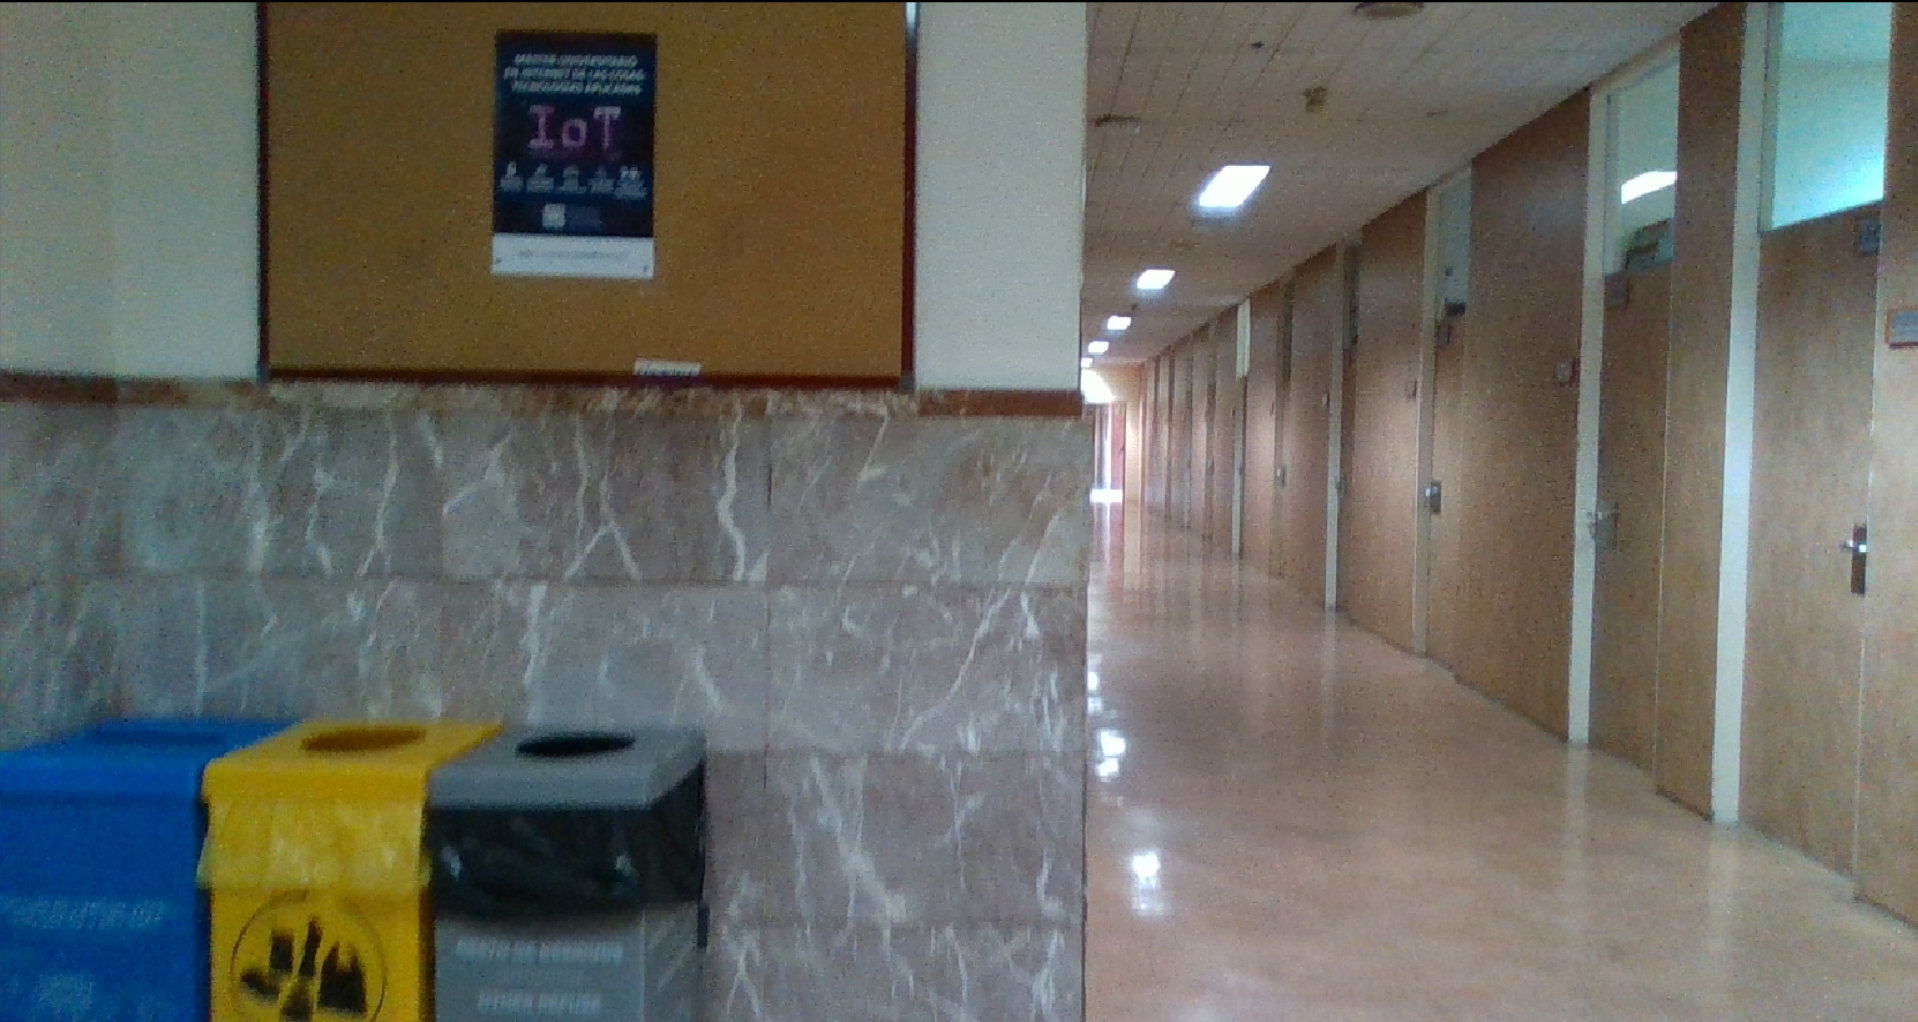
\includegraphics[width=\textwidth]{images/test1_visual.png}
        \caption{Imagen visual del ensayo, con la pared cercana en la parte izquierda de la escena.}
    \end{subfigure}

    \vspace{0.5em}

    \begin{subfigure}{0.95\textwidth}
        \centering
        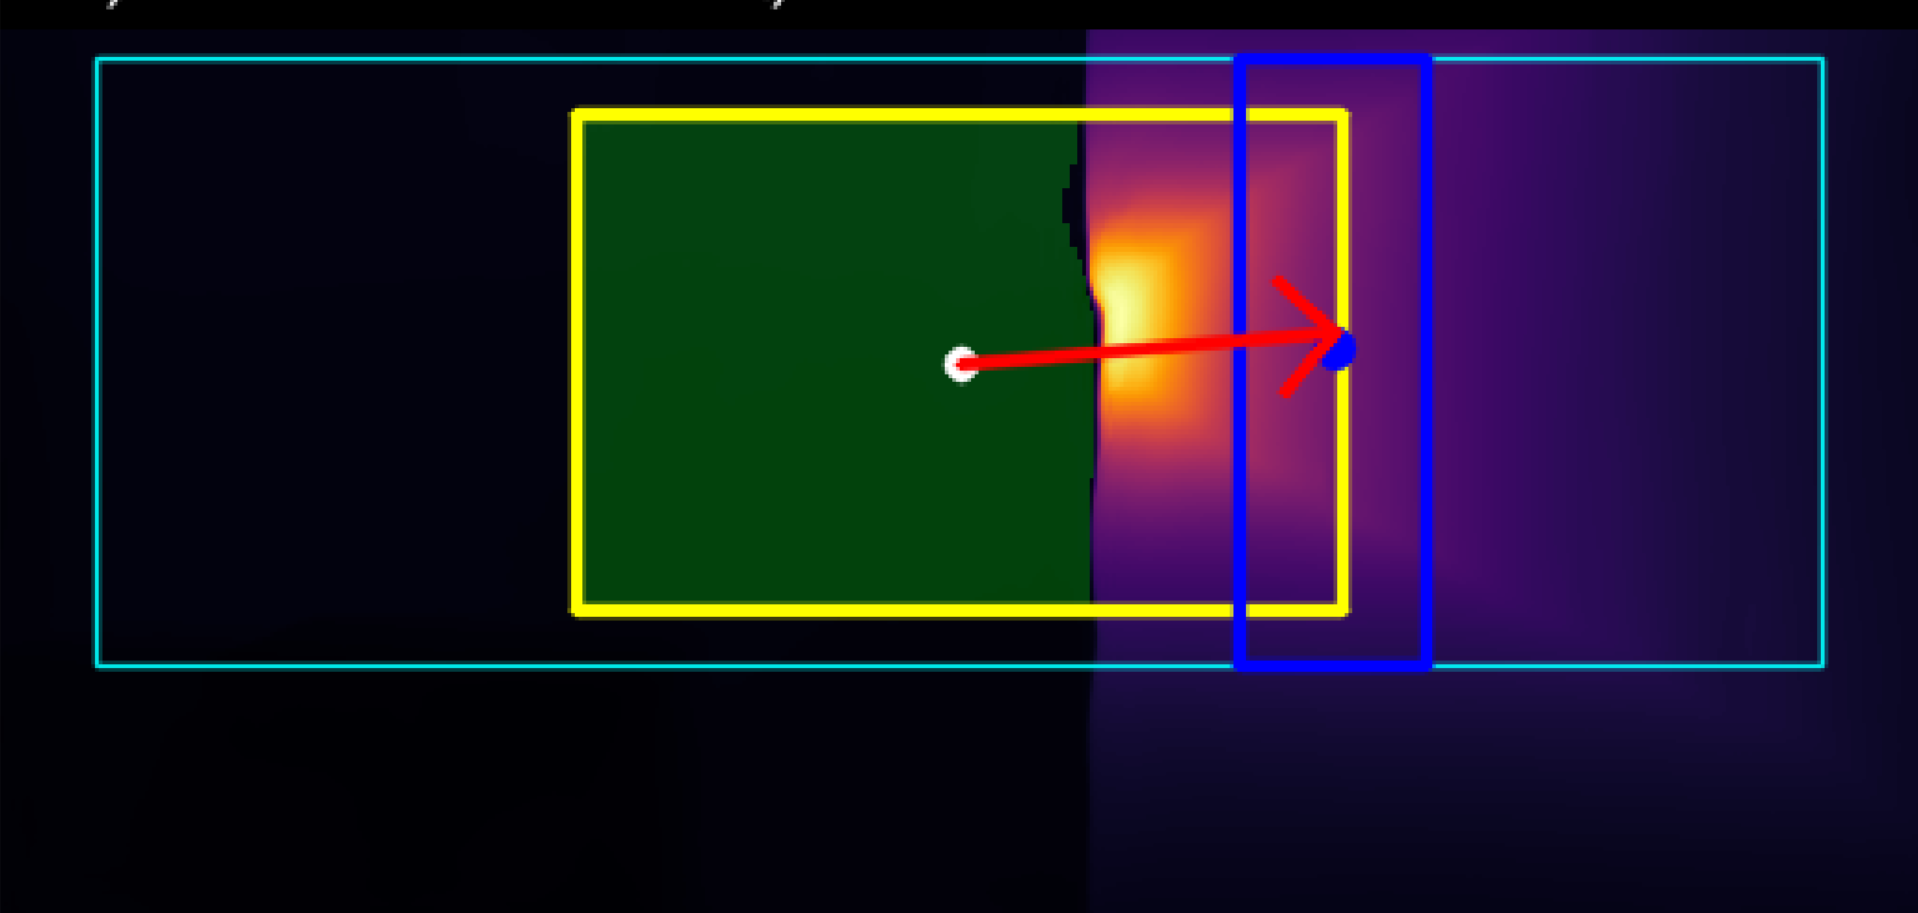
\includegraphics[width=\textwidth]{images/test1_prof.png}
        \caption{Estimaci\'on de profundidad y direcci\'on de evitaci\'on calculada hacia la derecha.}
    \end{subfigure}

    \vspace{0.5em}

    \begin{subfigure}{0.95\textwidth}
        \centering
        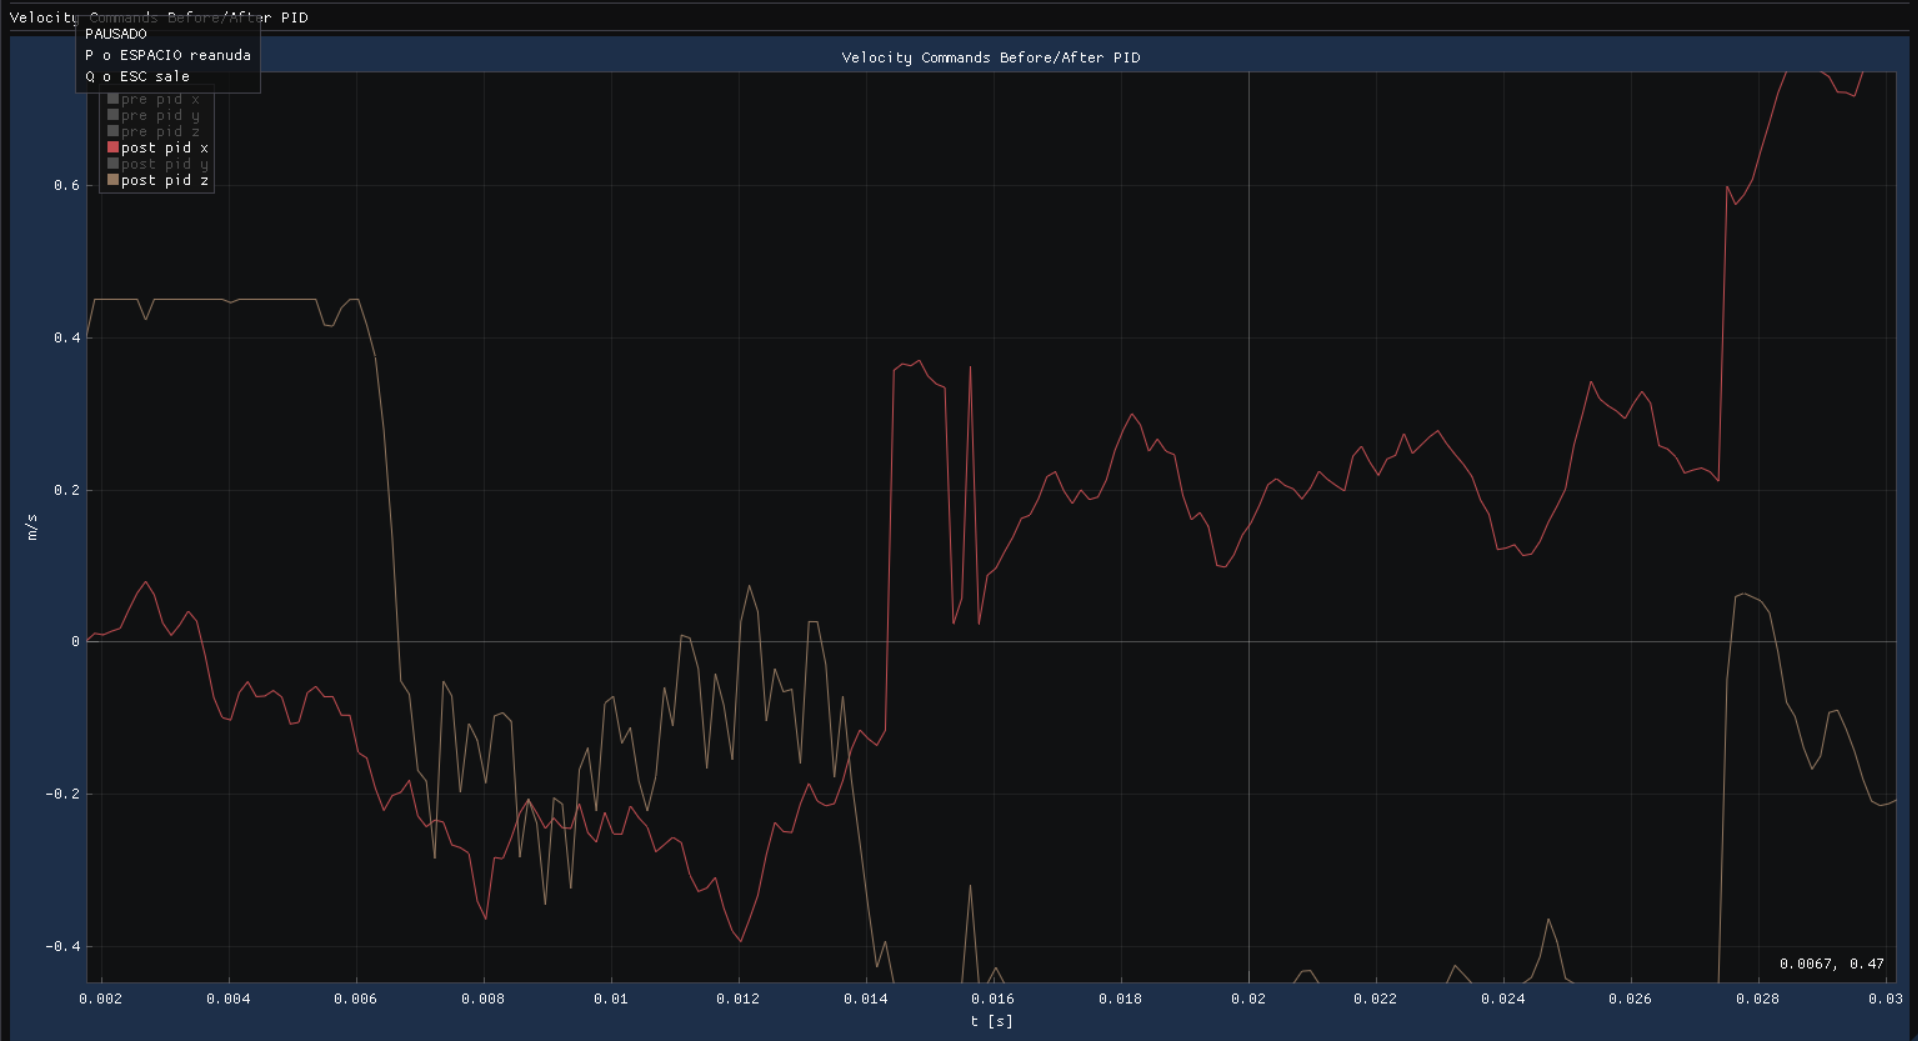
\includegraphics[width=\textwidth]{images/test1_vel_cmd.png}
        \caption{Comandos de velocidad, con \(x>0\) hacia la derecha y reducci\'on del avance en \(z\).}
    \end{subfigure}

    \caption{Resultados del Test 1. La escena visual, la salida del estimador de profundidad y los comandos de control son coherentes con una maniobra de evitaci\'on hacia la derecha ante la presencia de una pared cercana.}
    \label{fig:test1_evasion}
\end{figure}

\section{Test 2: Validaci\'on de la pre-integraci\'on mediante test sint\'eticos}
Este ensayo se ha realizado para validar de forma aislada la parte de pre-integraci\'on del estimador inercial. 
Para ello se a\~nadi\'o al proyecto un modo de funcionamiento en el que se proporciona un archivo csv con datos generados 
de manera sintética y donde se bloquea el cálculo visual. De esta forma, el resultado depende \'unicamente del modelo 
inercial y de su integraci\'on num\'erica.


Los ficheros sint\'eticos se generaron mediante un script en python. En dicho script se define 
una secuencia de aceleraciones lineales y velocidades angulares en el sistema del cuerpo, y a partir de ellas se integra 
una trayectoria de referencia conocida. Para mejorar la fidelidad de la simulaci\'on, la trayectoria se integra con un 
esquema de subpasos y usando una orientaci\'on intermedia en cada intervalo, reduciendo as\'i el error num\'erico del 
propio generador. Finalmente, para cada caso se calculan los incrementos esperados
\[
\Delta R = R_i^T R_j,\qquad
\Delta v = R_i^T\left(v_j-v_i\right),\qquad
\Delta p = R_i^T\left(p_j-p_i-v_i\Delta t\right),
\]
que se comparan con la salida del estimador implementado en el sistema.

Además, las medidas sint\'eticas se generarón mediante la inyección de ruido aleatorio basado en el que se cálculo con el 
método de Allan variance. El script permite inyectar tres contribuciones: sesgo est\'atico, ruido blanco y 
paseo aleatorio del sesgo. En t\'erminos pr\'acticos, cada muestra generada se modifica como
\[
\omega_m = \omega + b_g + b_g^{rw} + n_g,\qquad
a_m = a + b_a + b_a^{rw} + n_a,
\]
donde $b_g$ y $b_a$ son los sesgos constantes, $n_g$ y $n_a$ son ruidos blancos gaussianos y $b_g^{rw}$, $b_a^{rw}$ 
evolucionan como un random walk discreto. El ruido blanco se escala como $N/\sqrt{\Delta t}$ y el paseo aleatorio 
como $K\sqrt{\Delta t}$.

La Tabla~\ref{tab:test2_preintegration_summary} resume los resultados obtenidos para los seis casos sint\'eticos 
considerados. En ella se muestran la duraci\'on de cada secuencia, el n\'umero de muestras y el error final en 
posici\'on y orientaci\'on reportado por el programa de comparaci\'on.

\begin{table}[H]
    \centering
    \caption{Resumen de resultados del ensayo sint\'etico de pre-integraci\'on IMU.}
    \label{tab:test2_preintegration_summary}
    \small
    \resizebox{\textwidth}{!}{%
    \begin{tabular}{lcccc}
        \hline
        Caso & Duraci\'on [s] & Muestras & Error pos. [m] & Error rot. [$^\circ$] \\
        \hline
        \texttt{Caso 1: Movimiento cero} & 0.10 & 21 & $1.44\cdot10^{-5}$ & 0.0057 \\
        \texttt{Caso 2: Aceleración constante} & 0.10 & 21 & $1.44\cdot10^{-5}$ & 0.0057 \\
        \texttt{Caso 3: Giro constante} & 0.10 & 21 & $1.43\cdot10^{-5}$ & 0.0056 \\
        \texttt{Caso 4: Aceleración cte - Giro - Aceleración cte} & 0.10 & 21 & $1.43\cdot10^{-5}$ & 0.0057 \\
        \texttt{Caso 5: Camino complejo en los 6 GDL} & 2.00 & 401 & $3.34\cdot10^{-2}$ & 0.1861 \\
        \texttt{Caso 6: Camino complejo y de larga duración} & 69.00 & 13801 & 4.3690 & 0.2378 \\
        \hline
    \end{tabular}}
\end{table}


Los cuatro primeros casos son deliberadamente cortos y sencillos, y sirven para verificar que las tres componentes 
b\'asicas del modelo se comportan como se espera:

\paragraph{\texttt{Caso 1: Movimiento cero}}
En este caso no existe ni aceleraci\'on lineal ni velocidad angular, por lo que el resultado ideal es 
$\Delta p=\mathbf{0}$, $\Delta v=\mathbf{0}$ y $\Delta R=I$. El error obtenido es del orden de $10^{-5}\,\mathrm{m}$ en 
posici\'on y de unas pocas mil\'esimas de grado en rotaci\'on. Este resultado confirma que, en ausencia de maniobras, la 
implementaci\'on no introduce deriva apreciable a corto plazo y que la compensaci\'on de gravedad, sesgos y ruido se 
mantiene coherente.

\paragraph{\texttt{Caso 2: Aceleración constante}}
Se aplica una aceleraci\'on constante hacia delante, de modo que el incremento esperado es puramente traslacional. 
El error final vuelve a mantenerse en el orden de $10^{-5}\,\mathrm{m}$ y la rotaci\'on residual es pr\'acticamente 
la misma que en el caso de reposo. Esto indica que la integraci\'on de aceleraciones y la reconstrucci\'on de $\Delta v$ y 
$\Delta p$ son correctas para maniobras lineales simples.

\paragraph{\texttt{Giro constante}}
En este ensayo se impone una velocidad angular constante alrededor del eje de gui\~nada, sin traslaci\'on neta. El 
resultado esperado es una rotaci\'on pura, y la comparaci\'on muestra un error angular de s\'olo $0.0056^\circ$. 
La posici\'on permanece pr\'acticamente nula, con error tambi\'en del orden de $10^{-5}\,\mathrm{m}$. Por tanto, 
la integraci\'on de la actitud se considera correcta incluso con ruido y sesgos a\~nadidos.

\paragraph{\texttt{Aceleración cte - Giro - Aceleración cte}}
Este caso combina un tramo rectil\'ineo, un giro y un segundo tramo rectil\'ineo. Se trata de la primera prueba en la que 
aparecen simult\'aneamente traslaci\'on y rotaci\'on, aunque todav\'ia en una ventana temporal muy corta. El error se 
mantiene pr\'acticamente id\'entico al de los casos anteriores, lo que demuestra que el acoplamiento entre cinem\'atica 
lineal y angular est\'a bien resuelto en el horizonte corto.

Los dos \'ultimos casos son m\'as exigentes porque prolongan la integraci\'on durante mucho m\'as tiempo y fuerzan 
excitaci\'on en varios ejes:

\paragraph{\texttt{Camino complejo en los 6 GDL}}
La secuencia dura 2 segundos y encadena varios tramos con aceleraciones y velocidades angulares en distintos ejes. 
En este caso el error crece hasta aproximadamente $3.3\,\mathrm{cm}$ y $0.19^\circ$, lo cual es razonable al tratarse de 
una pre-integraci\'on pura sometida a ruido blanco, sesgos constantes y random walk. El resultado muestra que el modelo 
sigue siendo consistente cuando la maniobra excita simult\'aneamente varios grados de libertad.

\paragraph{\texttt{Camino complejo y de larga duración}}
Este es el caso m\'as severo del conjunto: una trayectoria de 69 segundos y 13801 muestras, con excitaci\'on prolongada 
en los tres ejes lineales y angulares. Como era esperable, aqu\'i se observa el mayor error acumulado, 
con $4.369\,\mathrm{m}$ en posici\'on y $0.238^\circ$ en orientaci\'on. El crecimiento del error confirma dos ideas 
importantes: por un lado, que la implementaci\'on es estable, ya que la orientaci\'on permanece muy cercana a la 
referencia incluso tras una secuencia larga; por otro, que una estimaci\'on basada s\'olo en IMU deriva de manera 
inevitable en posici\'on cuando no existe una observaci\'on externa que corrija los sesgos acumulados.

En conjunto, estos ensayos permiten concluir que la pre-integraci\'on implementada en el sistema reproduce 
correctamente el comportamiento esperado en maniobras simples y mantiene una consistencia muy alta en orientaci\'on 
incluso en secuencias largas y complejas. La deriva en posici\'on observada en los casos m\'as largos no debe 
interpretarse como un fallo del modelo, sino como el comportamiento esperable de una soluci\'on puramente inercial en 
presencia de ruido y sesgos. Precisamente por esta raz\'on resulta necesaria, en el sistema final, 
la correcci\'on peri\'odica aportada por la parte visual del estimador VIO.

\section{Test 3: Validaci\'on de la estimaci\'on solo visual}
En este caso se desactiva la parte inercial y se analiza el comportamiento del sistema cuando \'unicamente se emplea la 
informaci\'on visual. El objetivo principal es comprobar que la forma de la trayectoria estimada sea similar a la 
trayectoria real, aunque la escala pueda presentar un error residual debido a la ausencia de observaciones de 
informaci\'on inercial.

Como se observa en la Figura~\ref{fig:test3_visual_only}, la forma general de la trayectoria visual es similar a la del 
ground truth, por lo que el resultado es coherente con lo esperado para una estimaci\'on monocular. Sin embargo, tambi\'en 
se aprecia un error claro de escala, ya que la trayectoria estimada crece mucho m\'as que la real. Adem\'as, en los tramos 
con giro la estimaci\'on empeora m\'as, lo cual tambi\'en es esperable al no disponer de la informaci\'on angular m\'as 
precisa que aporta la IMU.


\begin{figure}[H]
    \centering
    \begin{subfigure}{0.95\textwidth}
        \centering
        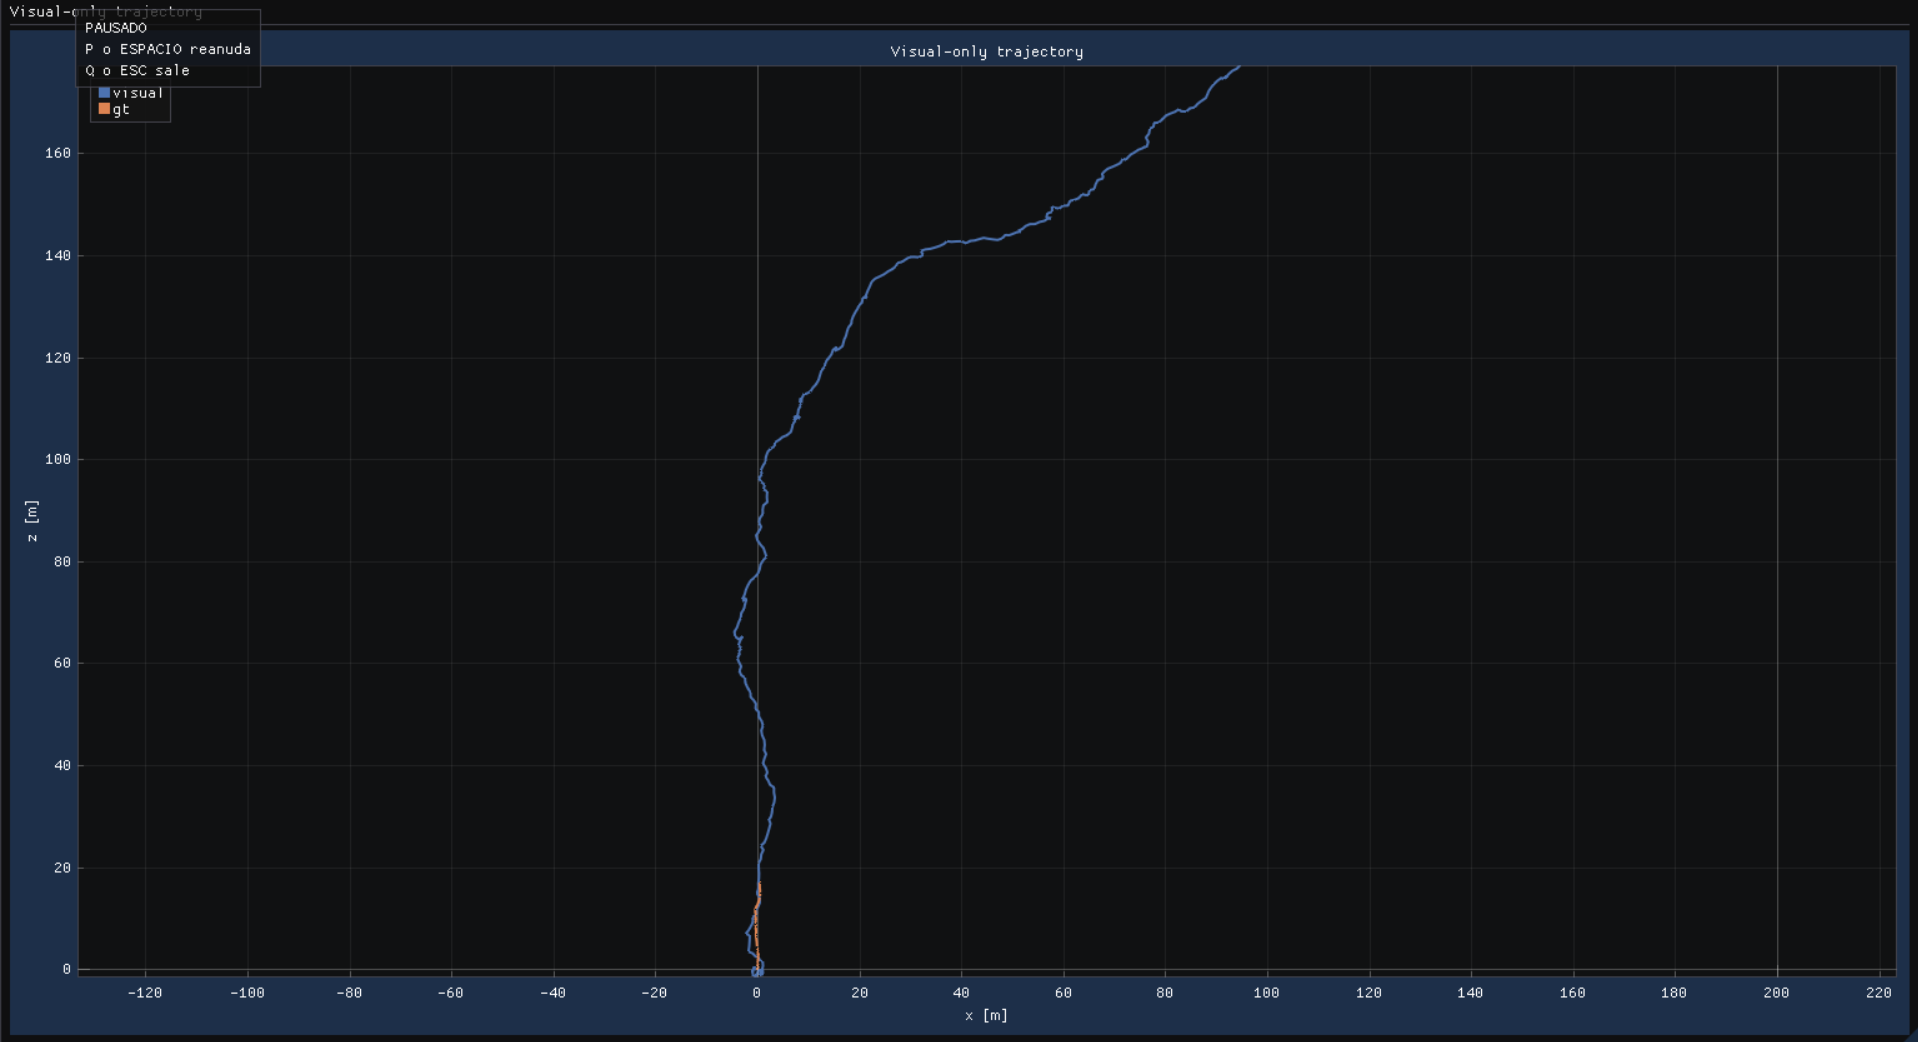
\includegraphics[width=\textwidth]{images/tezt3_gt_vis.png}
        \caption{Comparaci\'on directa entre la trayectoria visual y el ground truth.}
    \end{subfigure}

    \vspace{0.5em}

    \begin{subfigure}{0.95\textwidth}
        \centering
        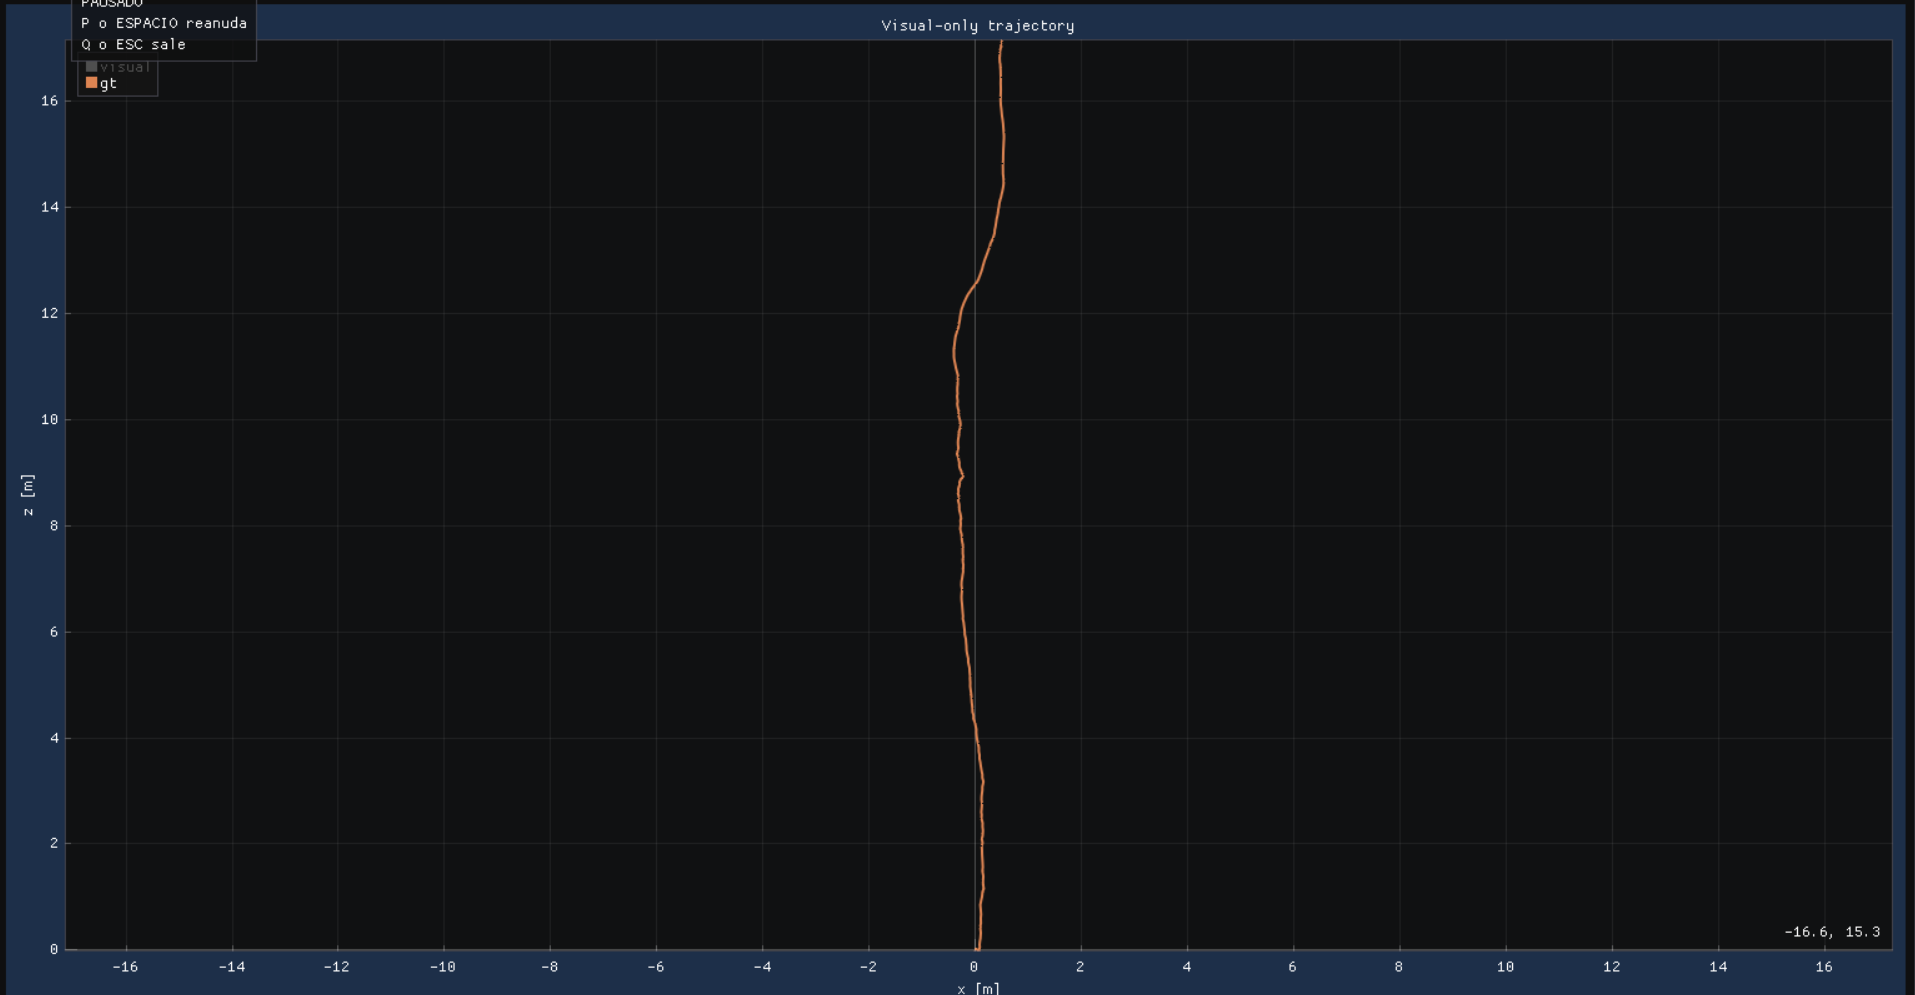
\includegraphics[width=\textwidth]{images/test3_solo_gt.png}
        \caption{Trayectoria de referencia.}
    \end{subfigure}

    \vspace{0.5em}

    \begin{subfigure}{0.95\textwidth}
        \centering
        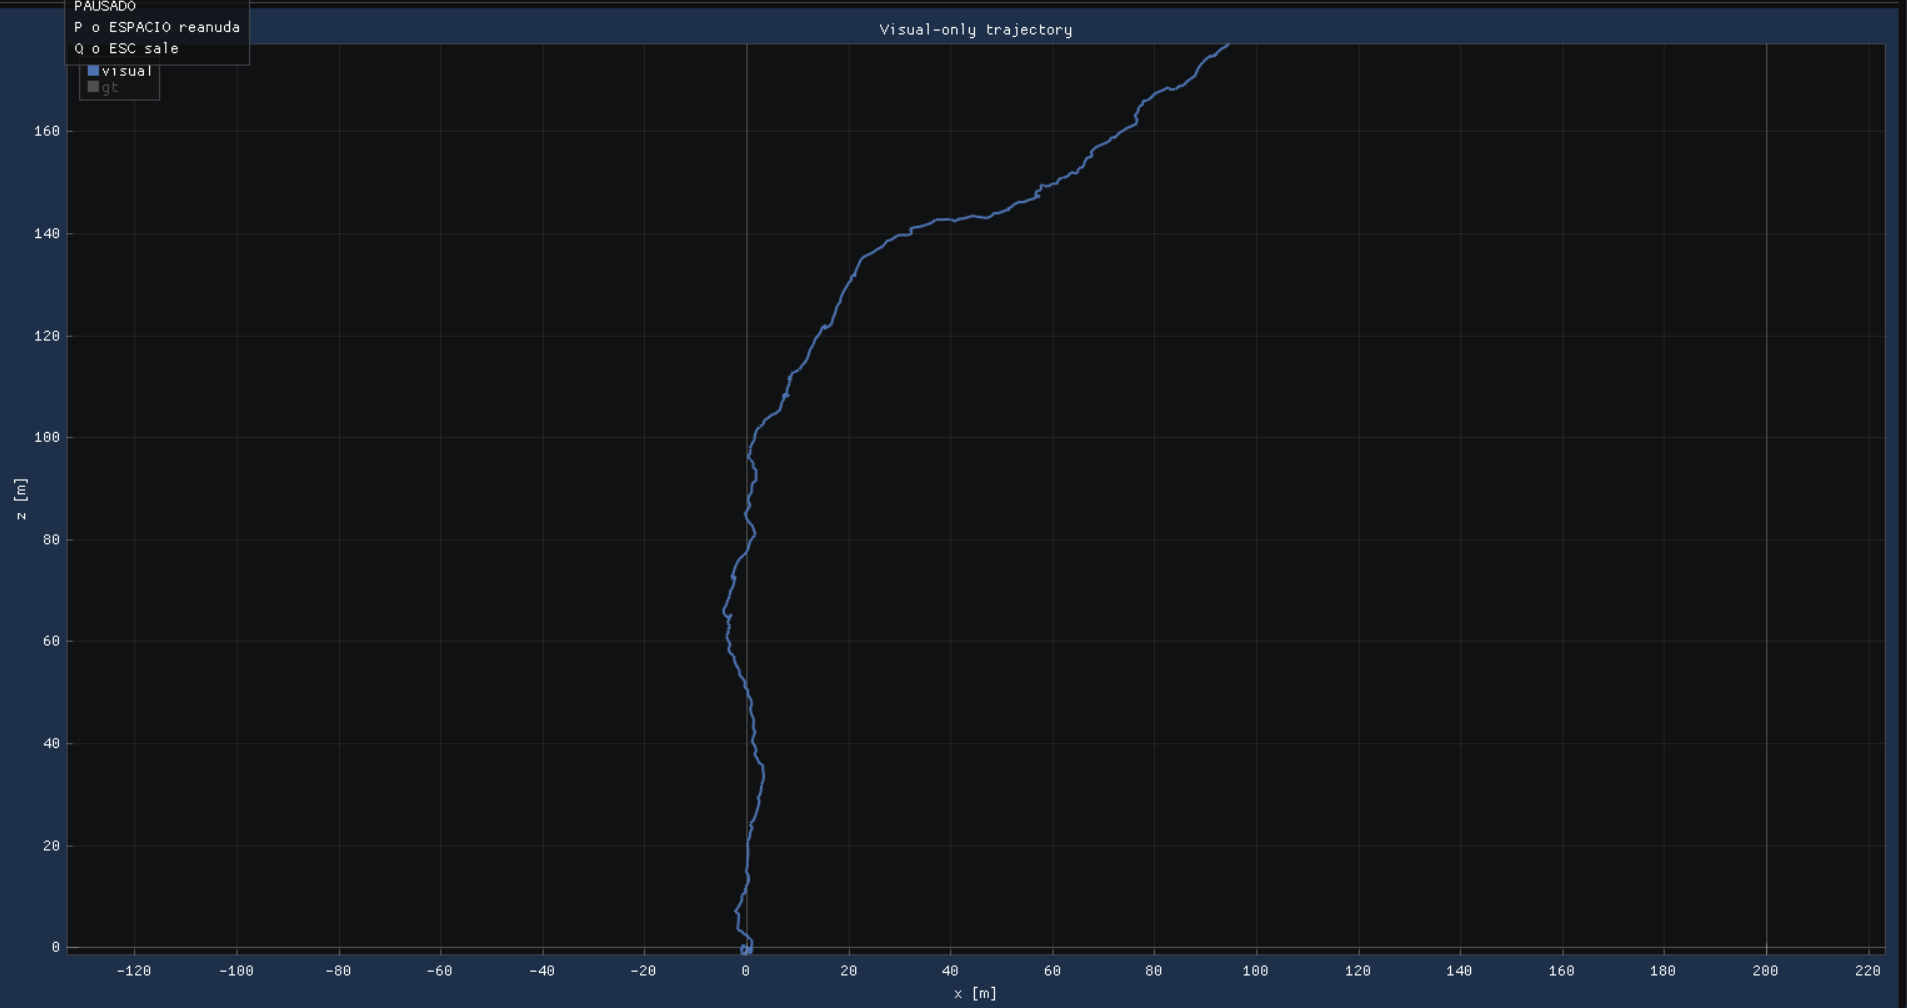
\includegraphics[width=\textwidth]{images/test3_solo_vis.png}
        \caption{Trayectoria estimada usando s\'olo informaci\'on visual.}
    \end{subfigure}

    \caption{Resultados del Test 3. La estimaci\'on visual reproduce la forma general de la trayectoria, pero presenta un error de escala apreciable y una mayor degradaci\'on en los tramos con giro.}
    \label{fig:test3_visual_only}
\end{figure}


\section{Test 4: Validaci\'on completa del sistema VIO}
En este ensayo se valida el funcionamiento completo del sistema VIO, comparando la trayectoria estimada con una referencia 
obtenida a partir del c\'alculo de posici\'on basado en el canal de profundidad. Conviene remarcar que esta referencia no 
es un ground truth exacto de la trayectoria real, sino una estimaci\'on alternativa, por lo que la trayectoria real 
esperable estar\'ia previsiblemente en un punto intermedio entre ambas.

Como se observa en la Figura~\ref{fig:test4_vio_full}, el sistema sigue una trayectoria coherente y cercana a la referencia. 
Adem\'as, en la Figura~\ref{fig:test4_vio_height} se aprecia que la estimaci\'on VIO mantiene mejor la altura que la 
referencia basada en profundidad. En esta gr\'afica la altura aparece invertida, por eso los valores se representan 
negativos.

\begin{figure}[H]
    \centering
    \begin{subfigure}{0.95\textwidth}
        \centering
        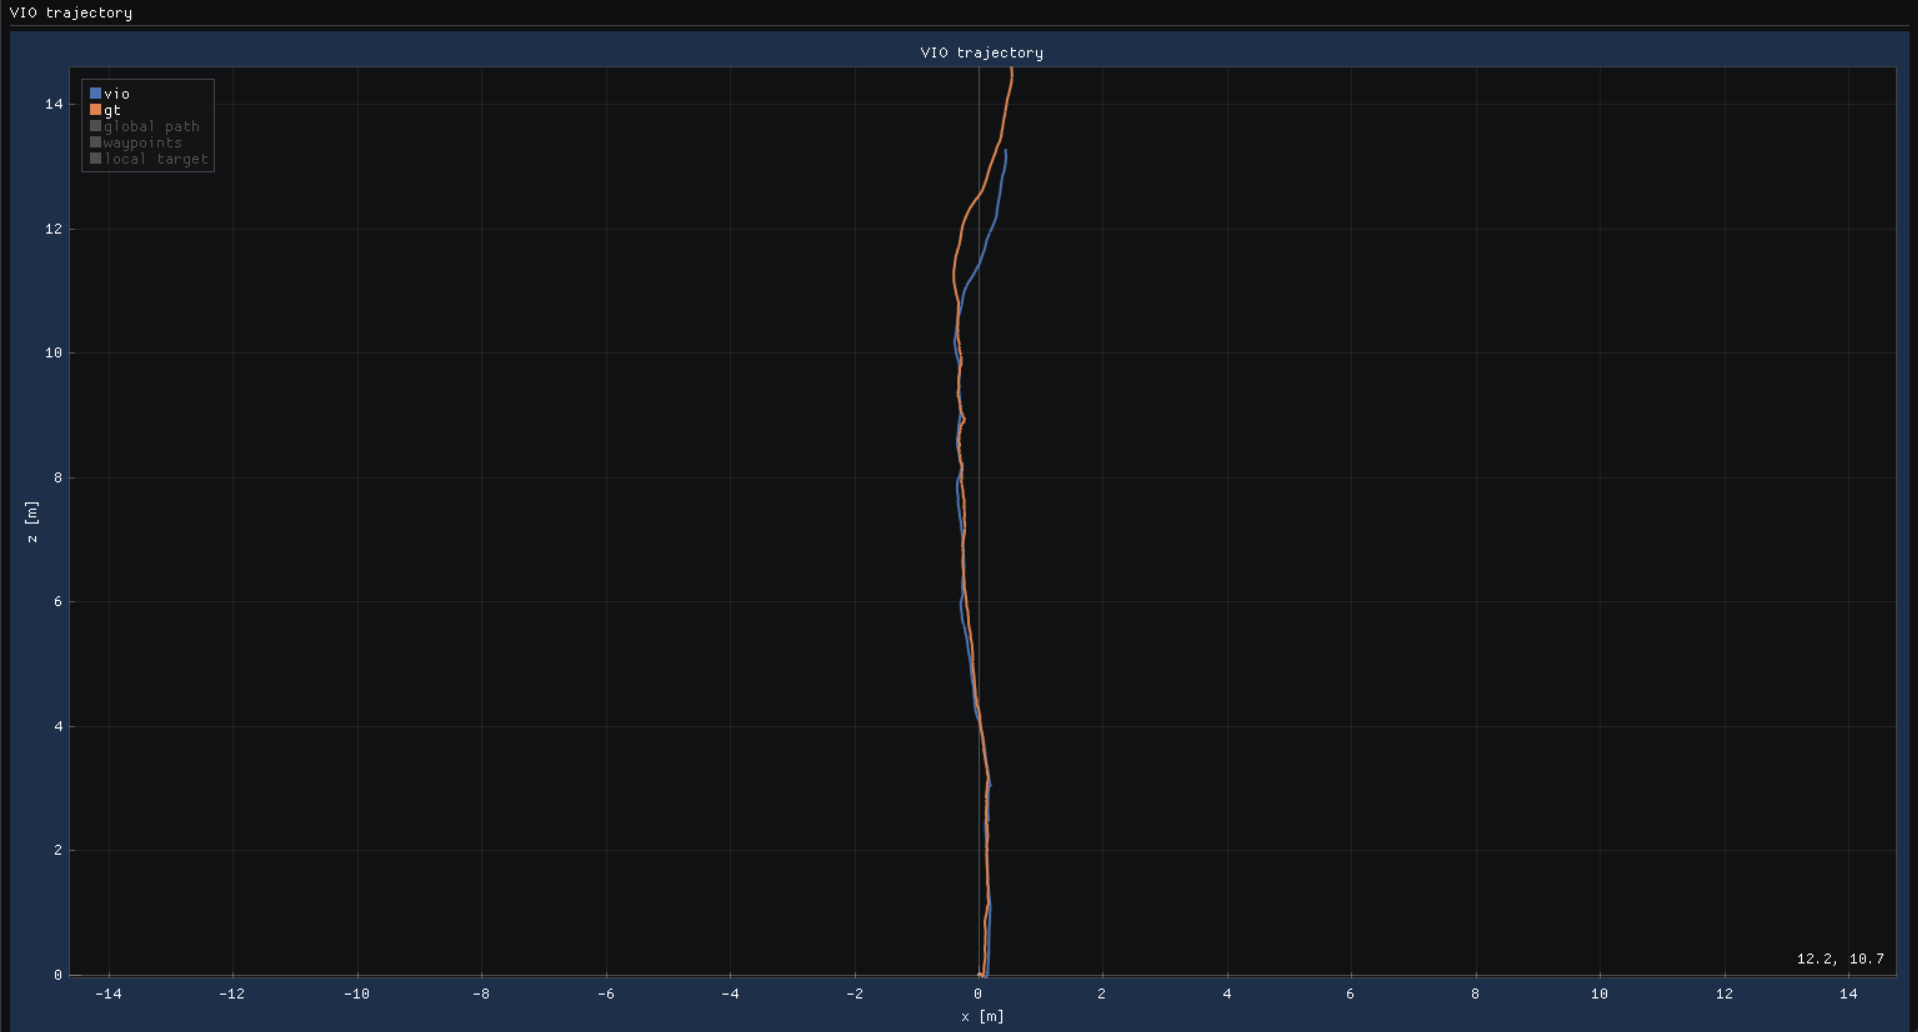
\includegraphics[width=\textwidth]{images/test4_fullvio.png}
        \caption{Comparaci\'on de la trayectoria estimada por el sistema VIO frente a la referencia basada en profundidad.}
    \end{subfigure}

    \vspace{0.5em}

    \begin{subfigure}{0.95\textwidth}
        \centering
        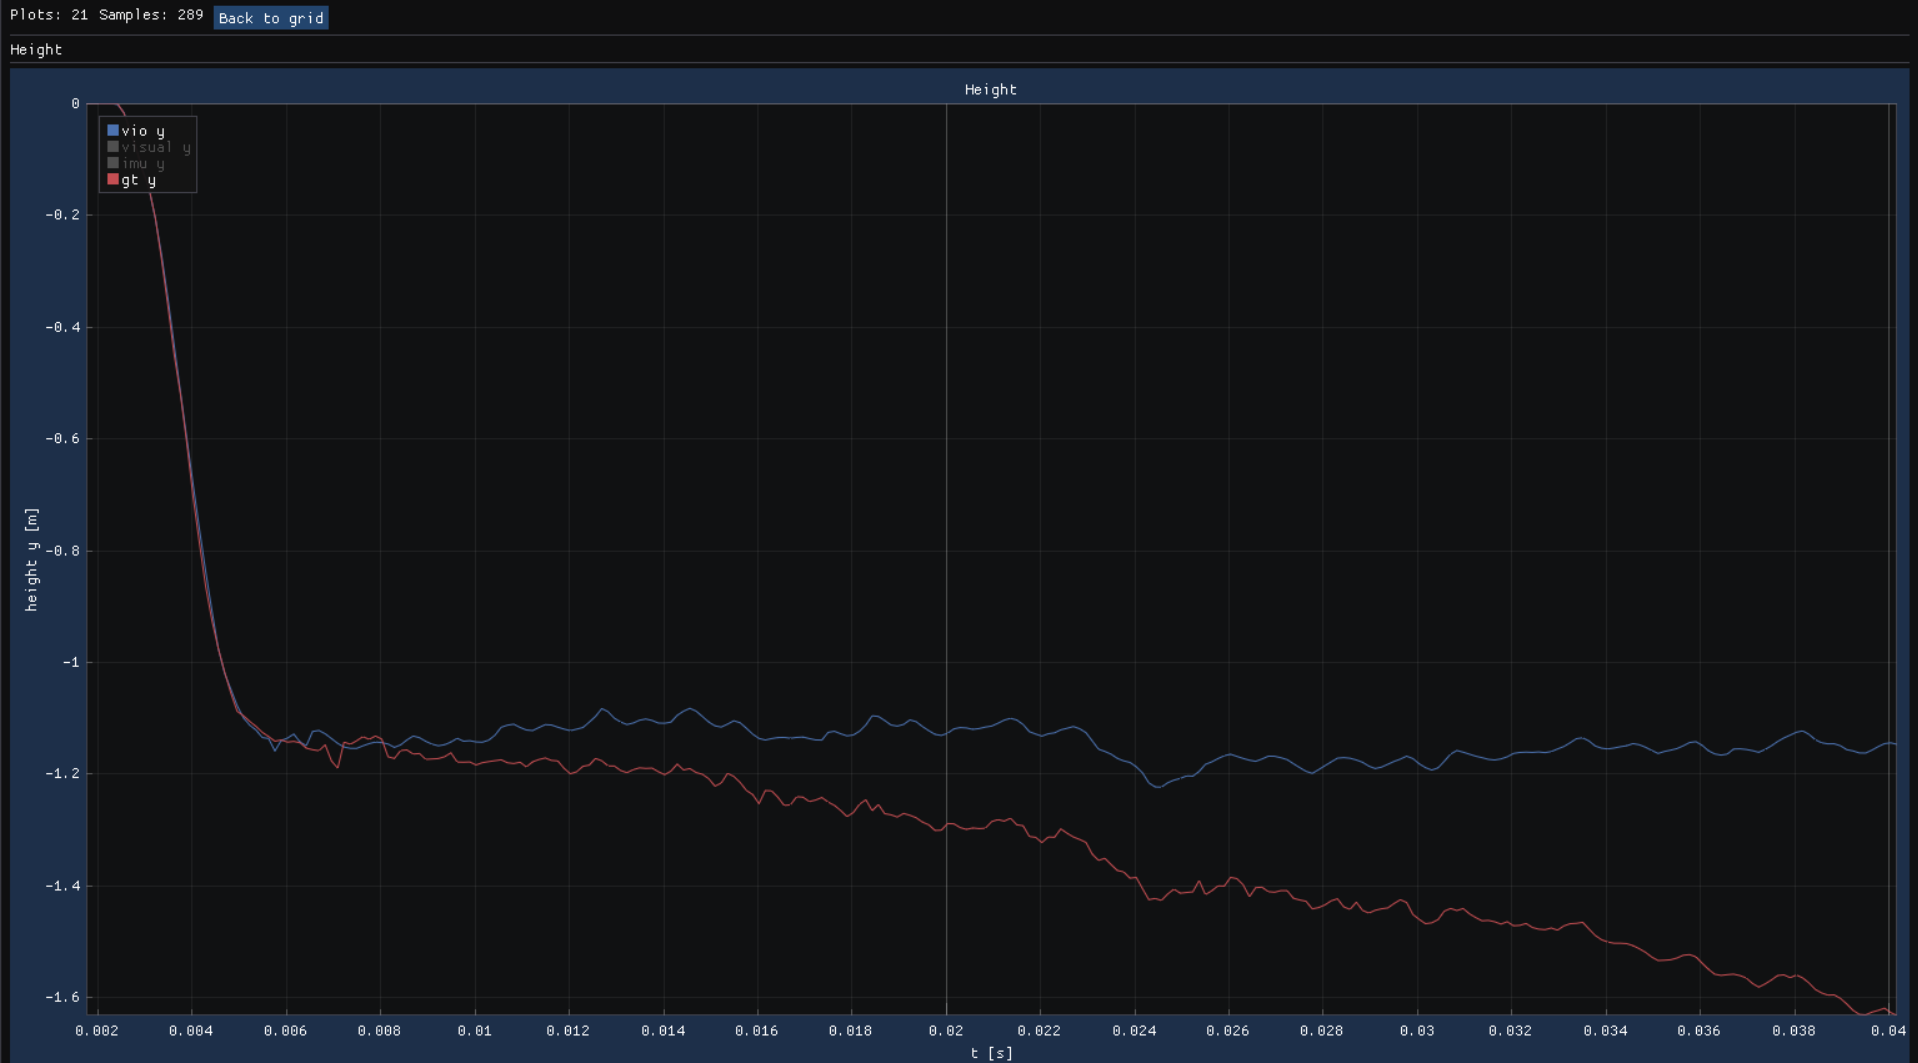
\includegraphics[width=\textwidth]{images/test4_altura.png}
        \caption{Comparaci\'on en altura. El eje aparece invertido, por lo que la altura se representa con valores negativos.}
        \label{fig:test4_vio_height}
    \end{subfigure}

    \caption{Resultados del Test 4. El sistema VIO mantiene una trayectoria global coherente y una estimaci\'on de altura m\'as estable, teniendo en cuenta que la referencia usada no constituye un ground truth exacto.}
    \label{fig:test4_vio_full}
\end{figure}

\section{Test 5: Validaci\'on de la frecuencia de control del sistema}
En este ensayo se ha medido la frecuencia de funcionamiento del sistema completo a partir del monitor de rendimiento 
implementado durante la ejecuci\'on. El objetivo es identificar qu\'e bloques dominan el coste temporal total y comprobar 
si la cadena de control mantiene una ejecuci\'on razonable para el escenario evaluado.

El resumen final muestra que el sistema completo procesa 289 iteraciones con un tiempo medio total de \(294.31\) ms, lo que 
equivale a una frecuencia media de \(3.40\) FPS. El cuello de botella principal se encuentra claramente en el bloque VIO, con 
un tiempo medio de \(186.71\) ms, seguido por el c\'alculo de ground truth, con \(93.26\) ms. En cambio, el m\'odulo DA3 
presenta un coste medio muy reducido, de \(2.48\) ms, y el bloque de control resulta pr\'acticamente despreciable frente al 
resto, con solo \(0.19\) ms de media.

Por tanto, puede concluirse que la limitaci\'on temporal del sistema no viene de la parte de control ni del estimador de 
profundidad, sino fundamentalmente del bloque de estimaci\'on VIO. Los valores m\'inimos y m\'aximos observados presentan una 
dispersi\'on elevada, por lo que resultan m\'as representativos los valores medios del resumen final que los picos instant\'aneos 
registrados durante la ejecuci\'on.


\begin{table}[H]
    \centering
    \caption{Resumen de tiempos y frecuencias medias del Test 5.}
    \label{tab:test5_frequencies}
    \small
    \resizebox{\textwidth}{!}{%
    \begin{tabular}{lcccc}
        \hline
        Bloque & Tiempo medio [ms] & FPS medio & Tiempo m\'in. [ms] & Tiempo m\'ax. [ms] \\
        \hline
        Source & 1.44 & 696.71 & 0.01 & 10.28 \\
        DA3 & 2.48 & 403.87 & 1.19 & 9.46 \\
        Ground truth & 93.26 & 10.72 & 5.12 & 300.99 \\
        VIO & 186.71 & 5.36 & 0.02 & 727.30 \\
        Control & 0.19 & 5301.89 & 0.08 & 13.15 \\
        Render & 10.51 & 95.17 & 6.09 & 33.76 \\
        Sistema completo & 294.31 & 3.40 & 7.43 & 925.43 \\
        \hline
    \end{tabular}}
\end{table}

\section{Test 6: Validaci\'on del funcionamiento del planificador global y local}
En este ensayo se muestra el funcionamiento conjunto del planificador global y del planificador local durante la 
ejecuci\'on del sistema. El objetivo es comprobar que el punto de seguimiento seleccionado por el planificador local sea 
coherente con la trayectoria global y que esa decisi\'on se refleje correctamente en los comandos de control.


Como se observa en la Figura~\ref{fig:test6_planning}, en la trayectoria se muestran en verde los puntos a seguir del 
planificador global y en morado el punto de seguimiento actual del planificador local. En el instante representado, dicho 
punto de seguimiento queda a la izquierda de la trayectoria del dron. De forma coherente con ello, en la gr\'afica de 
\texttt{yaw\_cmd} se aprecia que el comando de gui\~nada toma valores negativos para hacer girar el dron hacia ese lado, 
validando as\'i el funcionamiento esperado del sistema.

\begin{figure}[H]
    \centering
    \begin{subfigure}{0.95\textwidth}
        \centering
        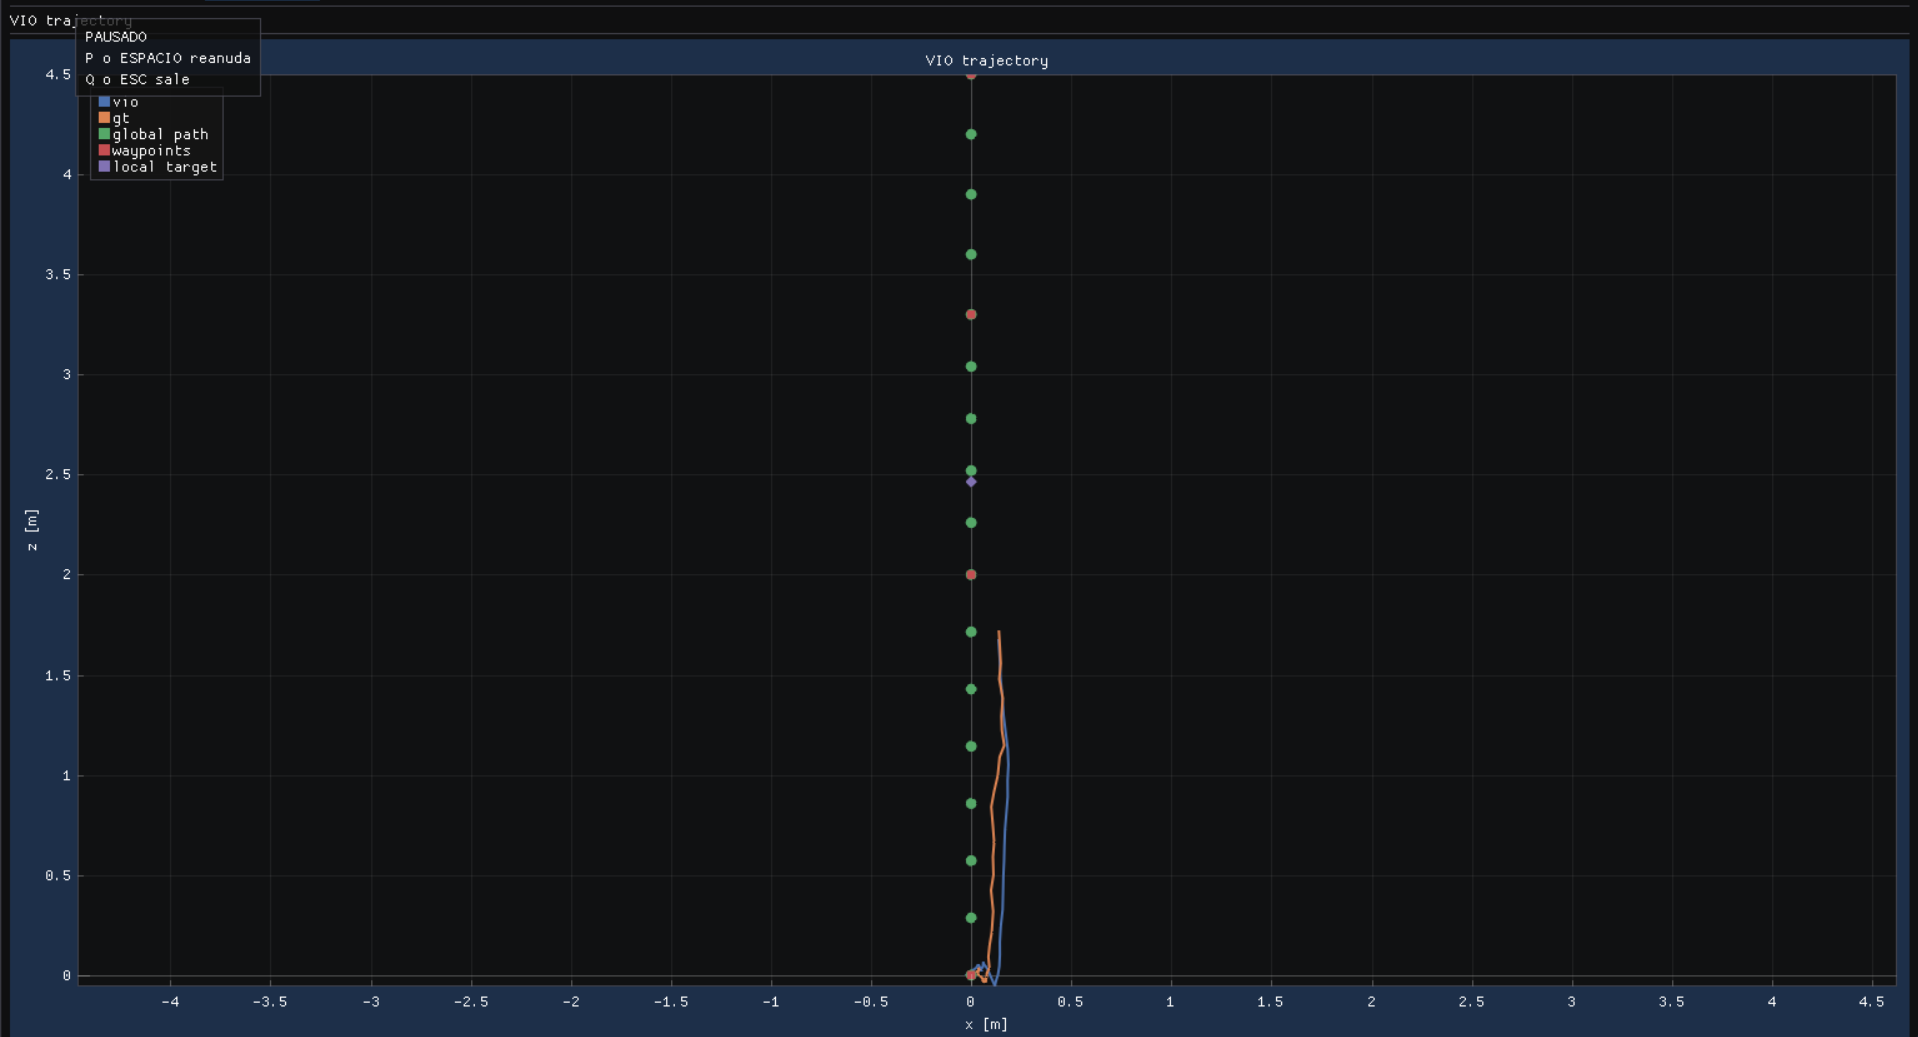
\includegraphics[width=\textwidth]{images/test6_planfiicacion.png}
        \caption{Trayectoria en un instante \(t\), con los puntos globales en verde y el punto de seguimiento local actual en morado.}
    \end{subfigure}

    \vspace{0.5em}

    \begin{subfigure}{0.95\textwidth}
        \centering
        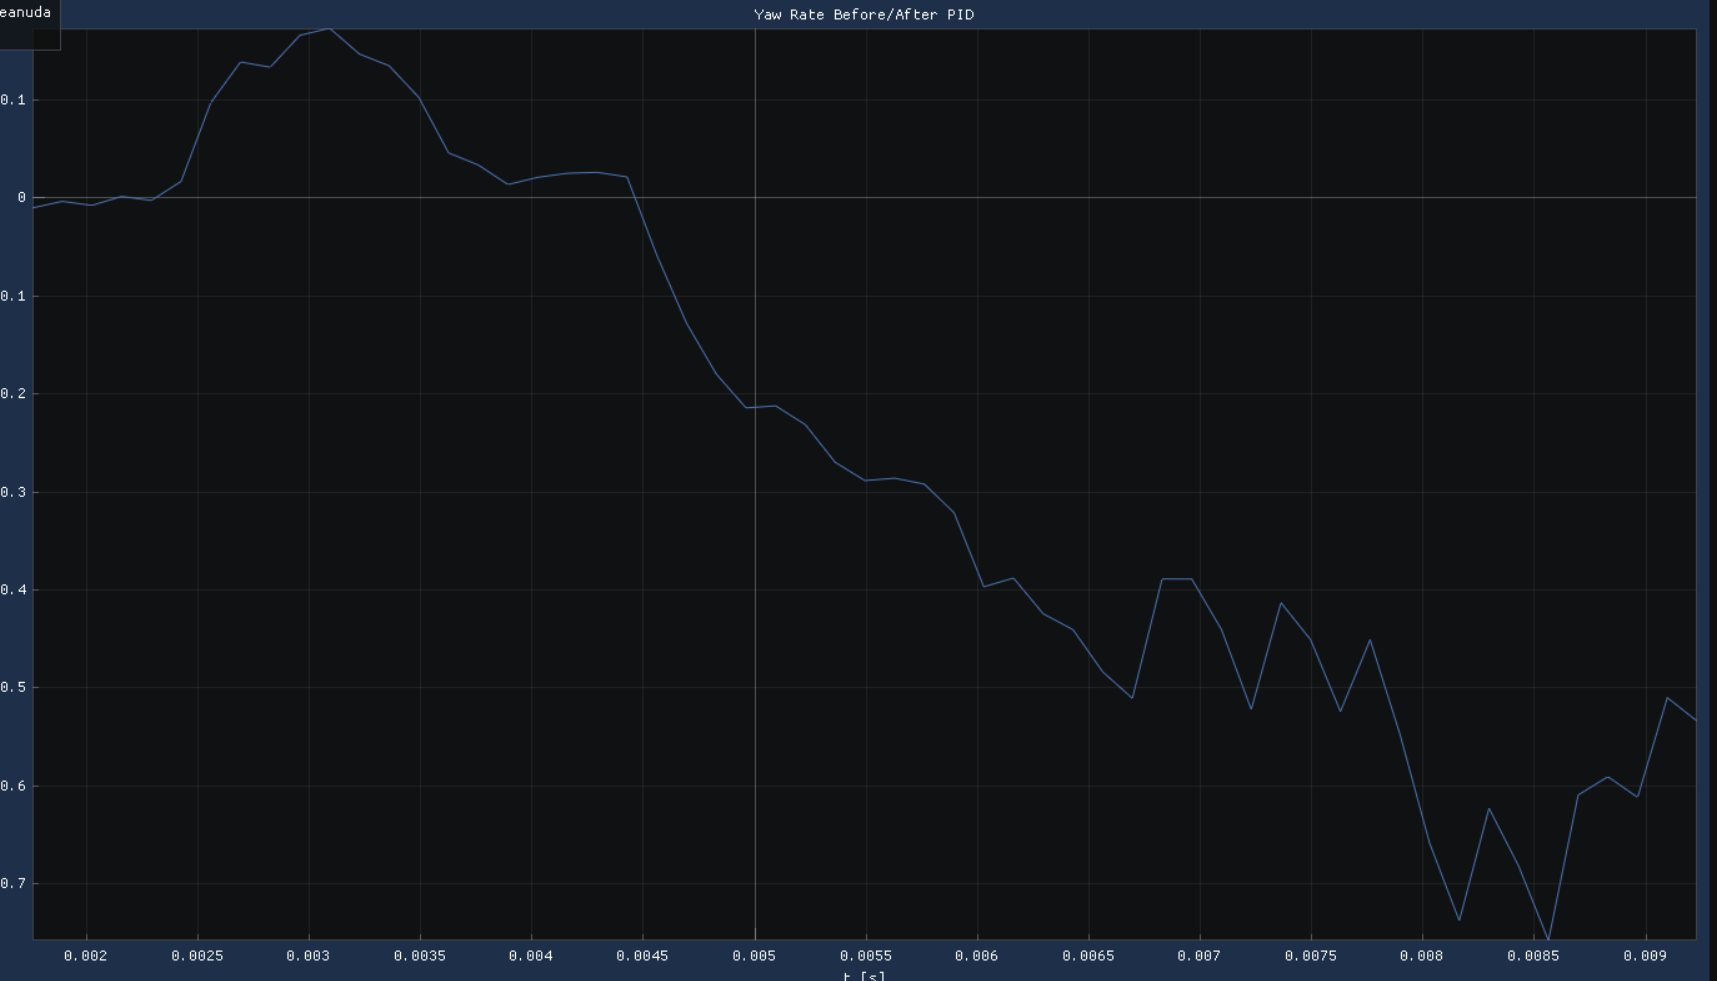
\includegraphics[width=\textwidth]{images/test6_yaw_cmd.png}
        \caption{Comando de \texttt{yaw}, que se hace negativo para girar hacia la izquierda.}
    \end{subfigure}

    \caption{Resultados del Test 6. La selecci\'on del punto de seguimiento por parte del planificador local y la respuesta del comando de gui\~nada son coherentes entre s\'i.}
    \label{fig:test6_planning}
\end{figure}

\chapter{Conclusiones y líneas futuras}

\section{Conclusiones}
\par
Este trabajo ha permitido desarrollar e integrar un sistema completo de navegaci\'on para un UAV en entornos interiores, 
combinando percepci\'on, estimaci\'on, planificaci\'on y control dentro de una misma arquitectura funcional. El resultado 
final no debe entenderse como una suma de bloques aislados, sino como una soluci\'on conjunta en la que cada m\'odulo aporta 
una parte necesaria para conseguir un comportamiento global coherente.

Desde el punto de vista de la arquitectura del sistema, se ha definido una separaci\'on adecuada entre la plataforma a\'erea 
y la estaci\'on de tierra, lo que ha permitido aprovechar mejor los recursos de c\'omputo disponibles y simplificar el 
desarrollo experimental. De forma complementaria, el sistema de comunicaciones implementado ha permitido transportar de 
manera estable la informaci\'on visual, inercial y de control, resolviendo de forma pr\'actica las necesidades del proyecto.

En la parte de estimaci\'on, el sistema de odometr\'ia visual-inercial desarrollado ha demostrado ser capaz de proporcionar 
una estimaci\'on de pose utilizable para navegaci\'on. Los ensayos realizados han mostrado tanto las ventajas de la fusi\'on 
visual-inercial en el sistema completo como las limitaciones de una soluci\'on puramente visual, especialmente en escala y 
en maniobras con giro. Esto confirma que la integraci\'on de la IMU aporta una mejora real en robustez y consistencia.

En paralelo, el estimador de profundidad y el sistema de evitaci\'on de obst\'aculos han permitido dotar al dron de una 
capacidad reactiva frente a obst\'aculos cercanos. Los resultados obtenidos muestran que la direcci\'on de evitaci\'on y los 
comandos generados son coherentes con la escena observada, lo que valida el enfoque adoptado para esta parte del problema.

Por otro lado, la capa de planificaci\'on y control ha permitido transformar una trayectoria global en referencias locales y, 
a partir de ellas, en comandos de velocidad ejecutables por el veh\'iculo. La validaci\'on experimental ha mostrado que el 
planificador local selecciona puntos de seguimiento coherentes con la trayectoria y que esta decisi\'on se refleja 
correctamente en los comandos de gui\~nada y movimiento.

Finalmente, el conjunto de ensayos realizados ha permitido validar de forma progresiva los distintos bloques del sistema, 
desde pruebas sint\'eticas de preintegraci\'on IMU hasta evaluaciones del sistema completo. En conjunto, puede concluirse 
que se han cumplido los objetivos principales del proyecto: disponer de una base funcional de navegaci\'on aut\'onoma para un 
UAV, integrar los distintos subsistemas en una \'unica cadena de funcionamiento y demostrar experimentalmente que el sistema 
responde de forma coherente en los escenarios evaluados.
No obstante, los ensayos temporales tambi\'en muestran que la frecuencia global de funcionamiento todav\'ia no es tan alta 
como ser\'ia deseable, especialmente por la carga computacional asociada al bloque VIO, por lo que el sistema a\'un presenta 
un margen claro de mejora en rendimiento.


\section{Líneas futuras}

A partir de los resultados obtenidos en este trabajo, se identifican varias líneas de mejora que podrían abordarse en desarrollos futuros. 
Aunque la solución propuesta permite avanzar hacia una navegación segura de un UAV en entornos interiores, todavía presenta ciertas 
limitaciones. Por ello, a continuación se recogen algunos puntos de mejora que, por cuestiones de tiempo o por quedar fuera del alcance 
definido para este proyecto, no se han desarrollado en profundidad, pero que podrían aportar un valor significativo a la solución propuesta:

\begin{itemize}
    \item Optimizar computacionalmente el sistema, en especial el bloque de odometr\'ia visual-inercial y el c\'alculo de referencia, para aumentar la frecuencia global de funcionamiento y acercar la soluci\'on a un comportamiento m\'as pr\'oximo a tiempo real.
    \item Desarrollar un sistema VI-SLAM completo, incorporando la generación de un mapa del entorno y técnicas de \textit{loop closure}.
    \item Implementar un planificador global que tenga en cuenta el mapa del entorno y genere una trayectoria en función de la construcción del mapa en línea.
    \item Aumentar el tiempo de calibración mediante varianza de Allan hasta, al menos, 24 a 48 horas, con el objetivo de obtener una caracterización más precisa de la IMU.
    \item Implementar una interfaz gráfica de control que permita utilizar el algoritmo de forma más visual e intuitiva.
    \item Explorar e investigar algoritmos de planificación más avanzados para UAV en entornos interiores.
    \item Validación experimental en escenarios interiores más complejos.
\end{itemize}


% --- BIBLIOGRAFÍA ---
\clearpage
\addcontentsline{toc}{chapter}{Bibliografía}
% \setquotestyle[english]{british}
\printbibliography

% --- ANEXOS ---
\appendix
% !TeX root = ../memoria.tex
\chapter{Curvas de desviación de Allan de la IMU}
\label{anexo:allan}

En este anexo se recogen las curvas de desviación de Allan obtenidas para los tres ejes del
acelerómetro y los tres ejes del giróscopo. Estas curvas se emplearon para estimar los
parámetros de ruido blanco \(N\) y paseo aleatorio del sesgo \(K\) utilizados en la
configuración del estimador VIO.

\begin{figure}[p]
    \centering
    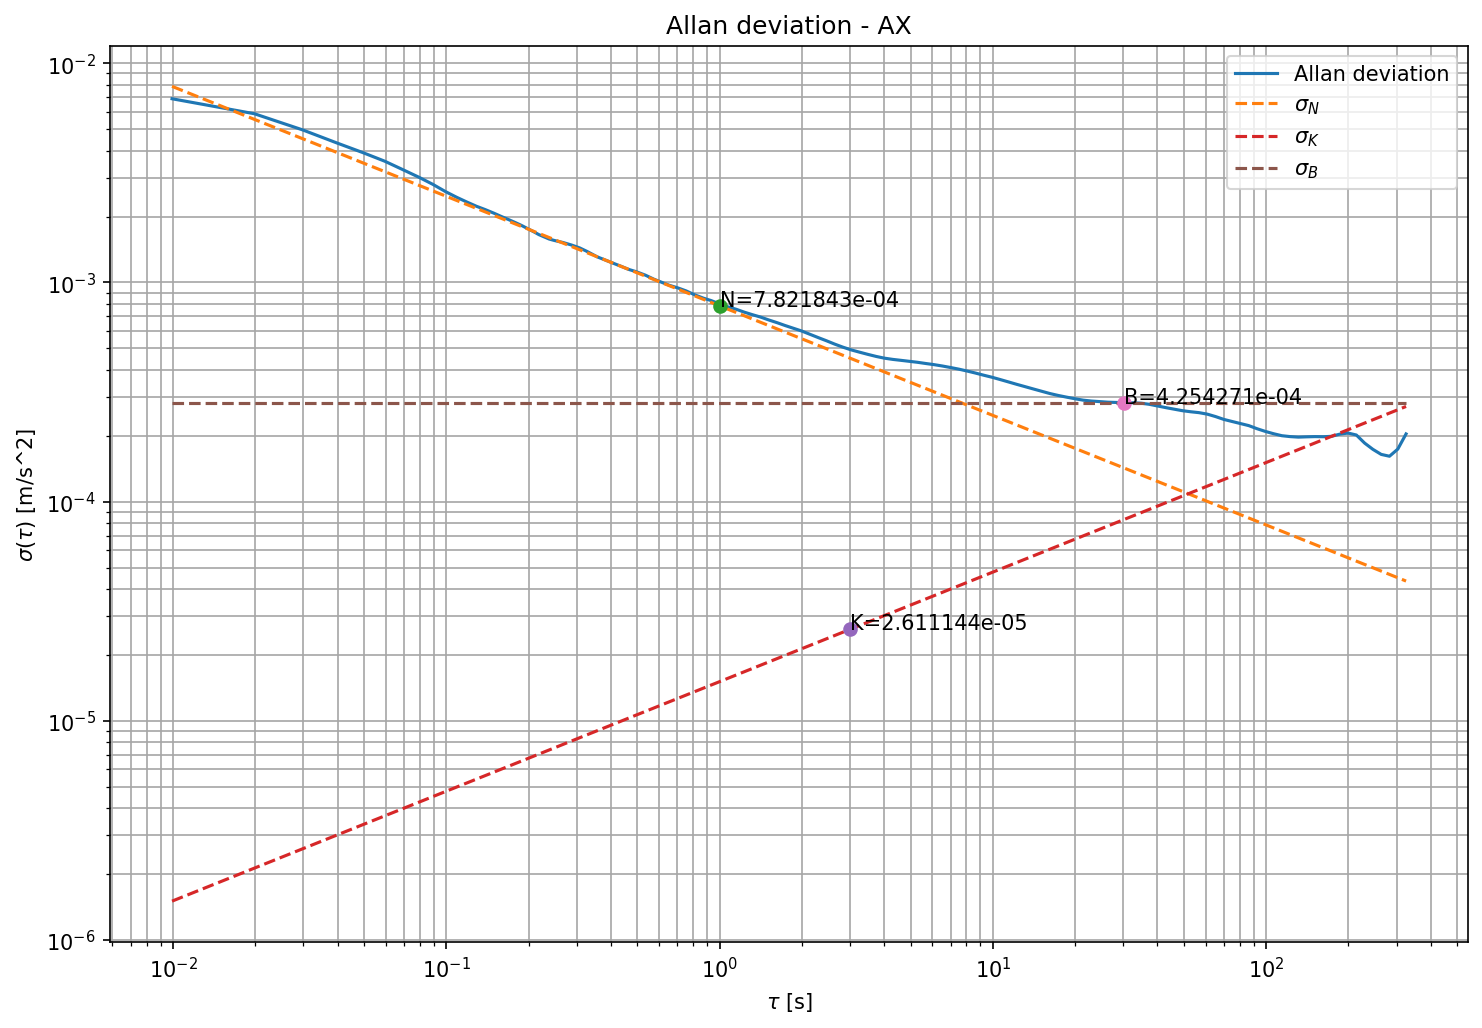
\includegraphics[width=0.88\textwidth]{images/ax_allan.png}
    \caption{Curva de desviación de Allan correspondiente al eje \(x\) del acelerómetro durante el ensayo estático de una hora.}
    \label{fig:allan_ax_anexo}
\end{figure}

\begin{figure}[p]
    \centering
    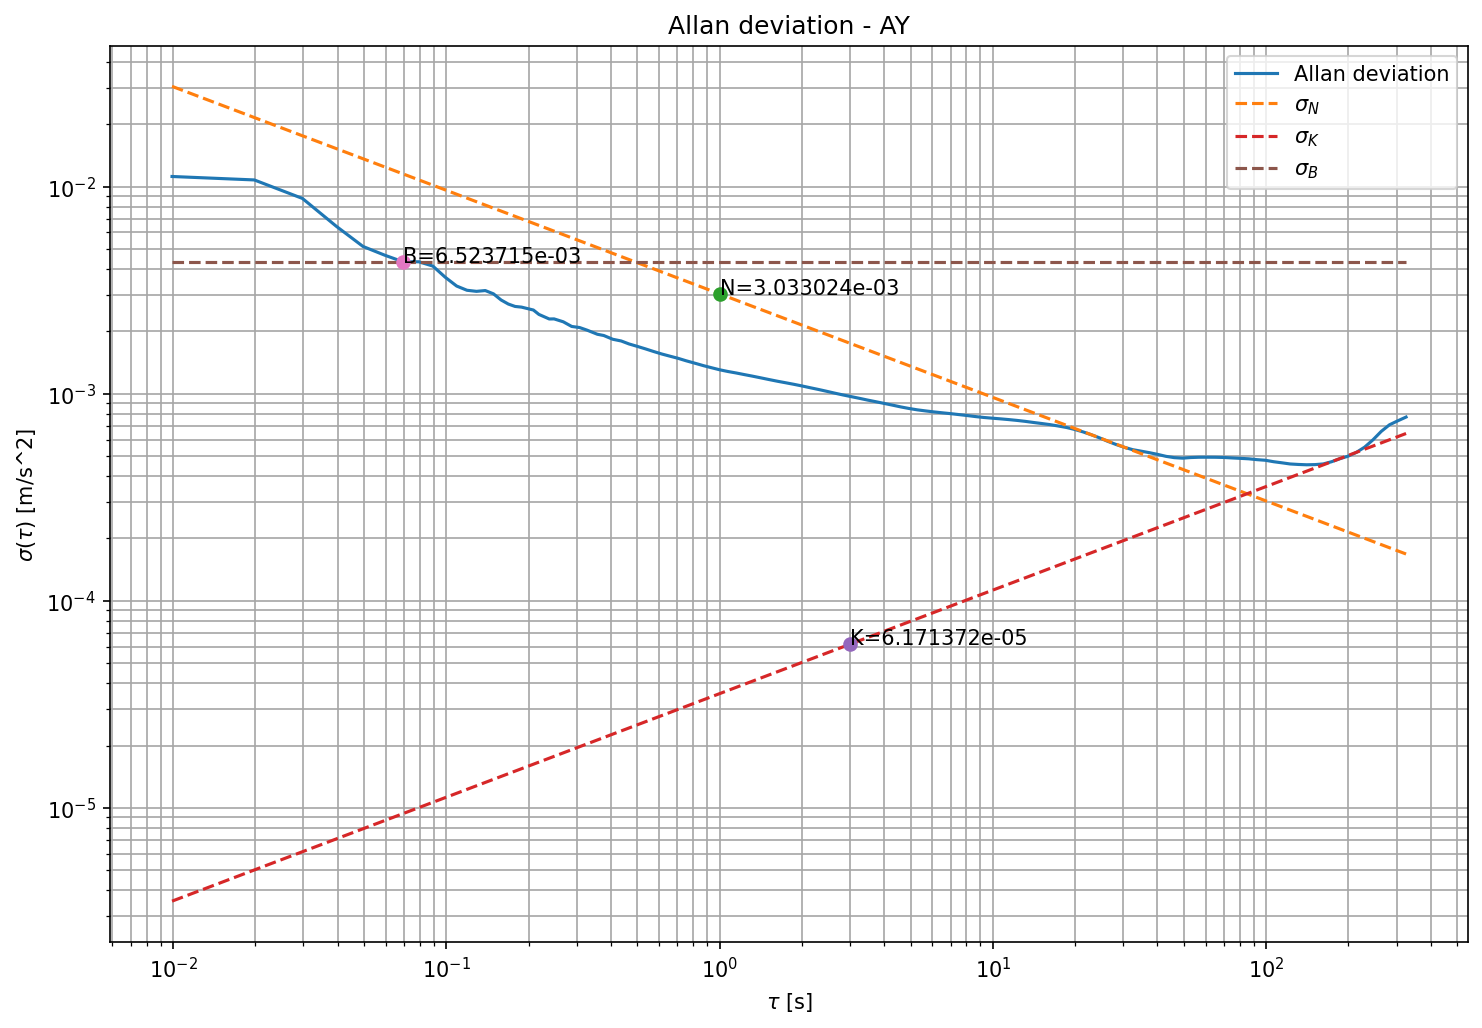
\includegraphics[width=0.88\textwidth]{images/ay_allan.png}
    \caption{Curva de desviación de Allan correspondiente al eje \(y\) del acelerómetro durante el ensayo estático de una hora.}
    \label{fig:allan_ay_anexo}
\end{figure}

\begin{figure}[p]
    \centering
    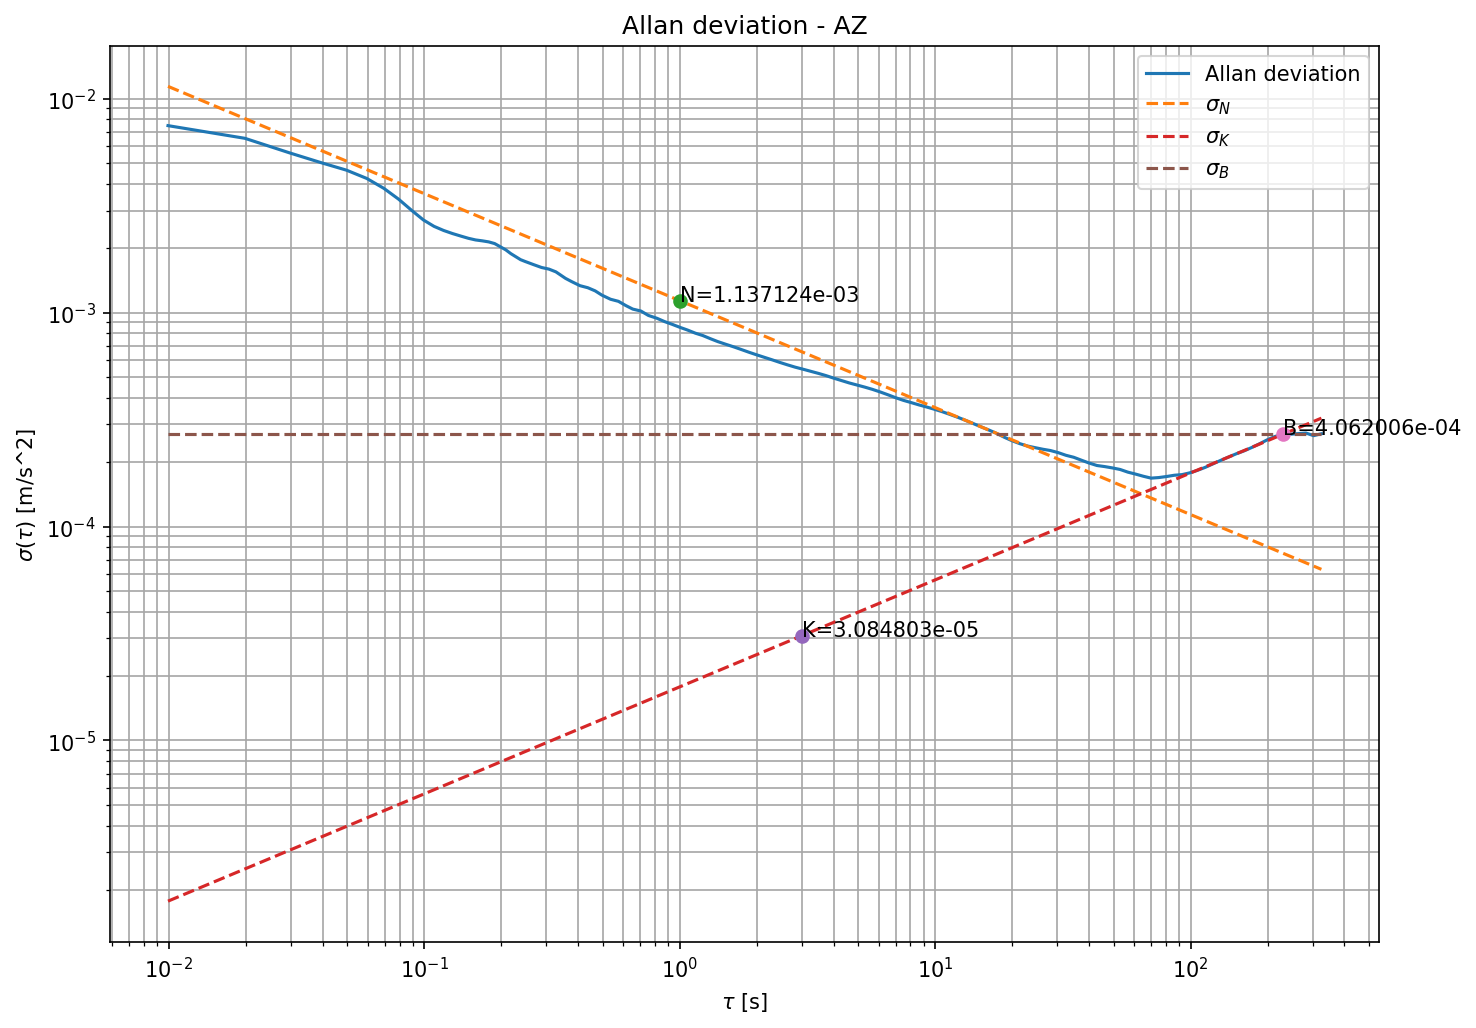
\includegraphics[width=0.88\textwidth]{images/az_allan.png}
    \caption{Curva de desviación de Allan correspondiente al eje \(z\) del acelerómetro durante el ensayo estático de una hora.}
    \label{fig:allan_az_anexo}
\end{figure}

\begin{figure}[p]
    \centering
    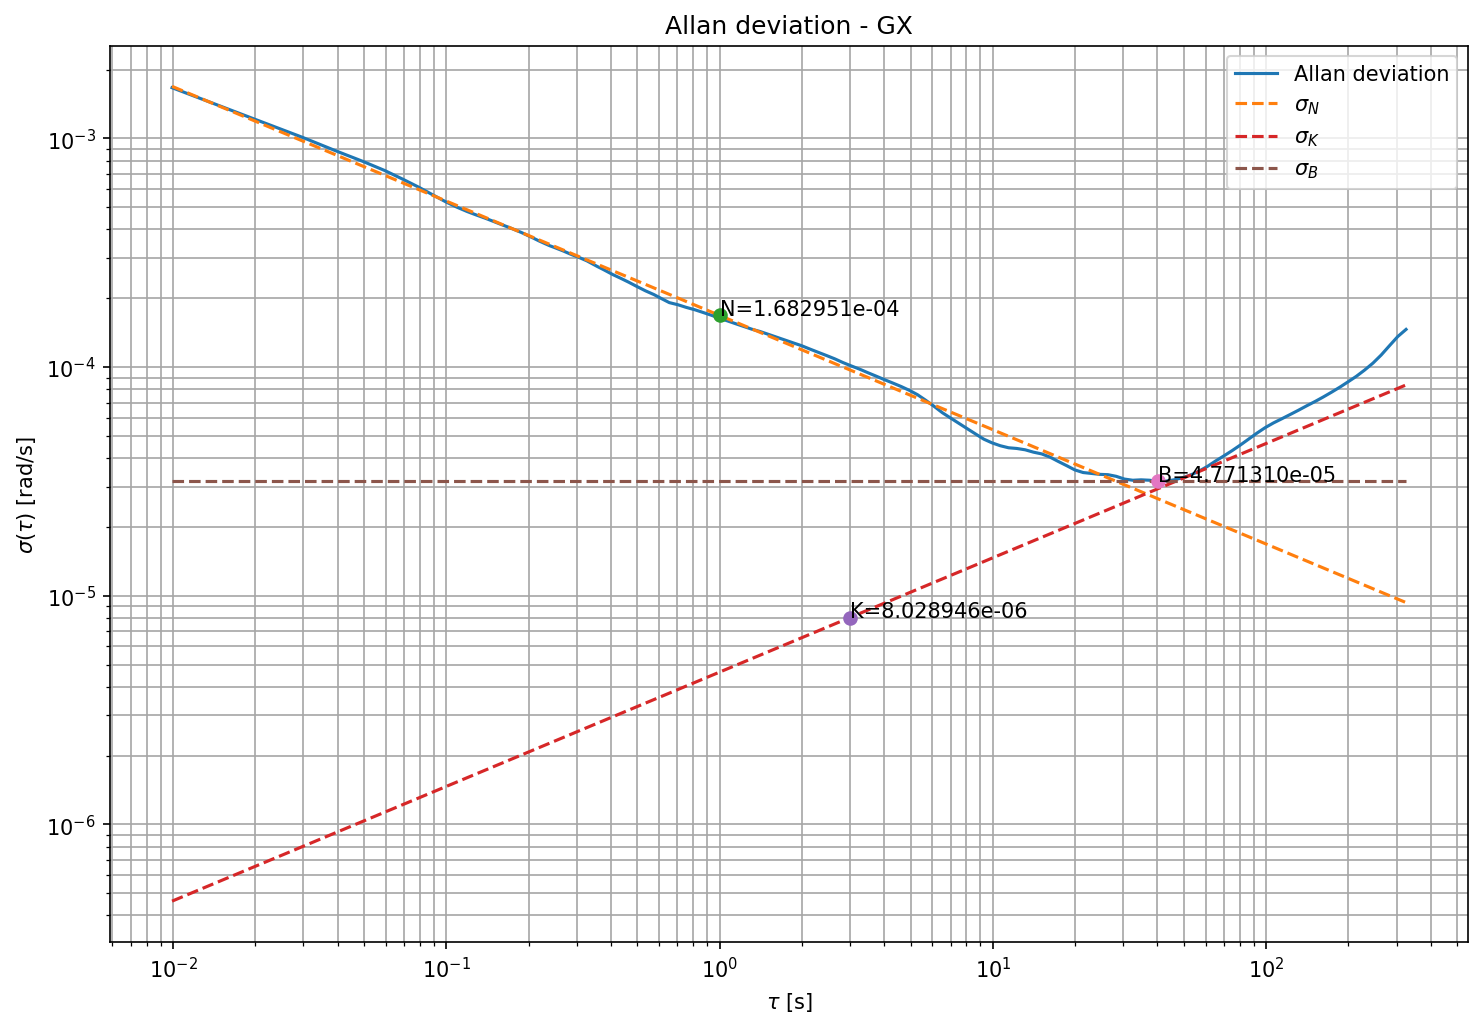
\includegraphics[width=0.88\textwidth]{images/gx_allan.png}
    \caption{Curva de desviación de Allan correspondiente al eje \(x\) del giróscopo durante el ensayo estático de una hora.}
    \label{fig:allan_gx_anexo}
\end{figure}

\begin{figure}[p]
    \centering
    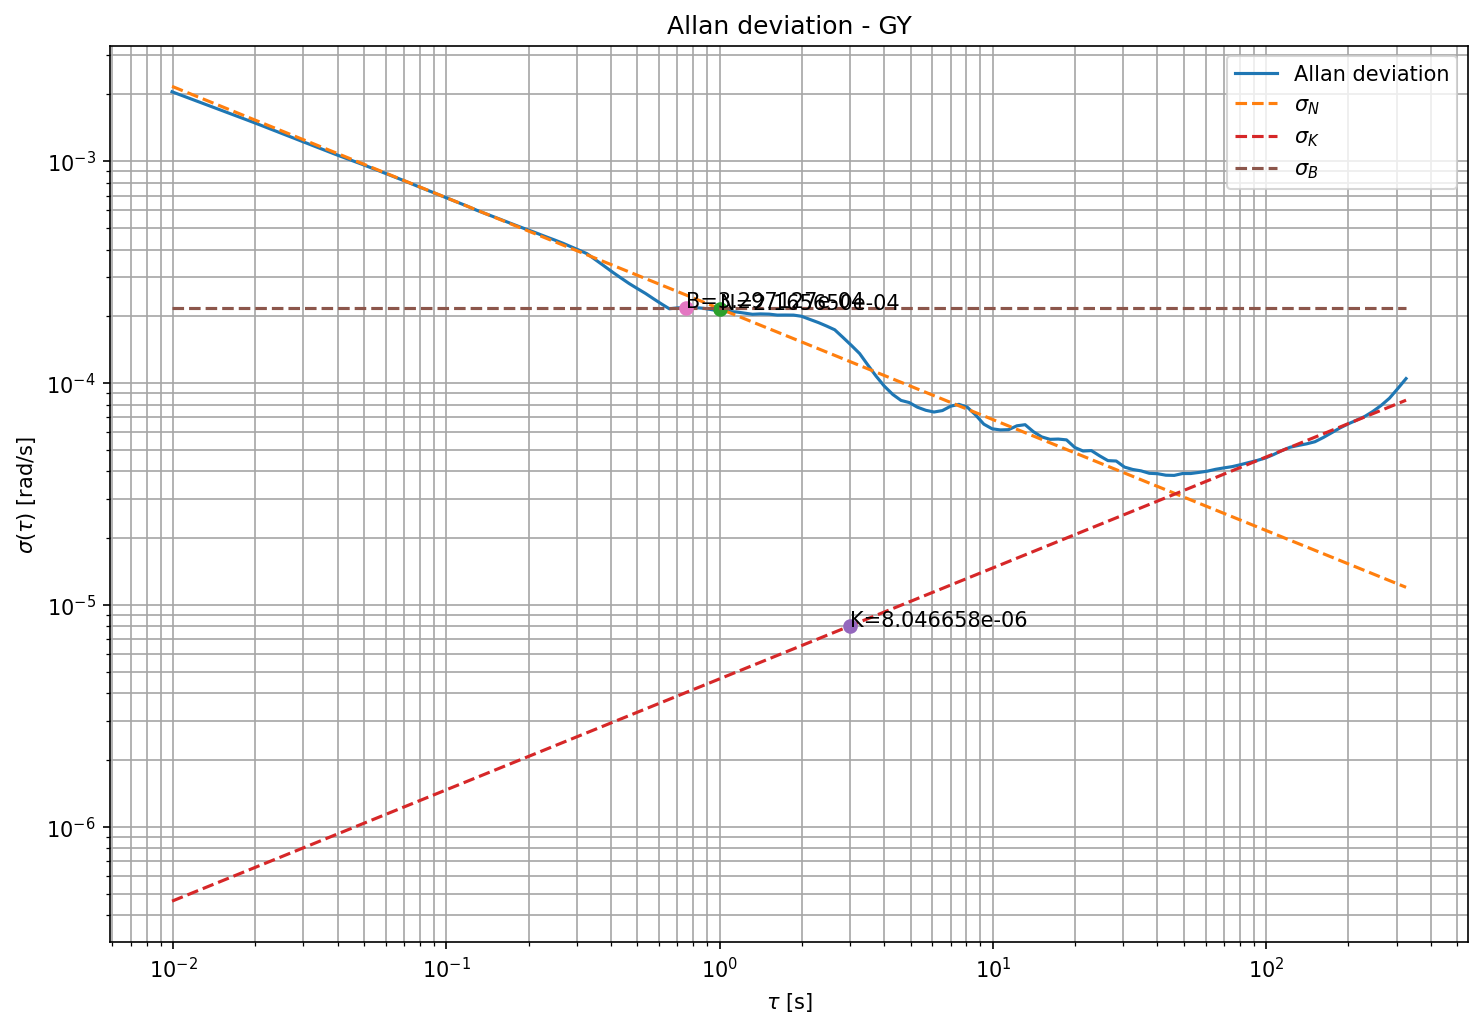
\includegraphics[width=0.88\textwidth]{images/gy_allan.png}
    \caption{Curva de desviación de Allan correspondiente al eje \(y\) del giróscopo durante el ensayo estático de una hora.}
    \label{fig:allan_gy_anexo}
\end{figure}

\begin{figure}[p]
    \centering
    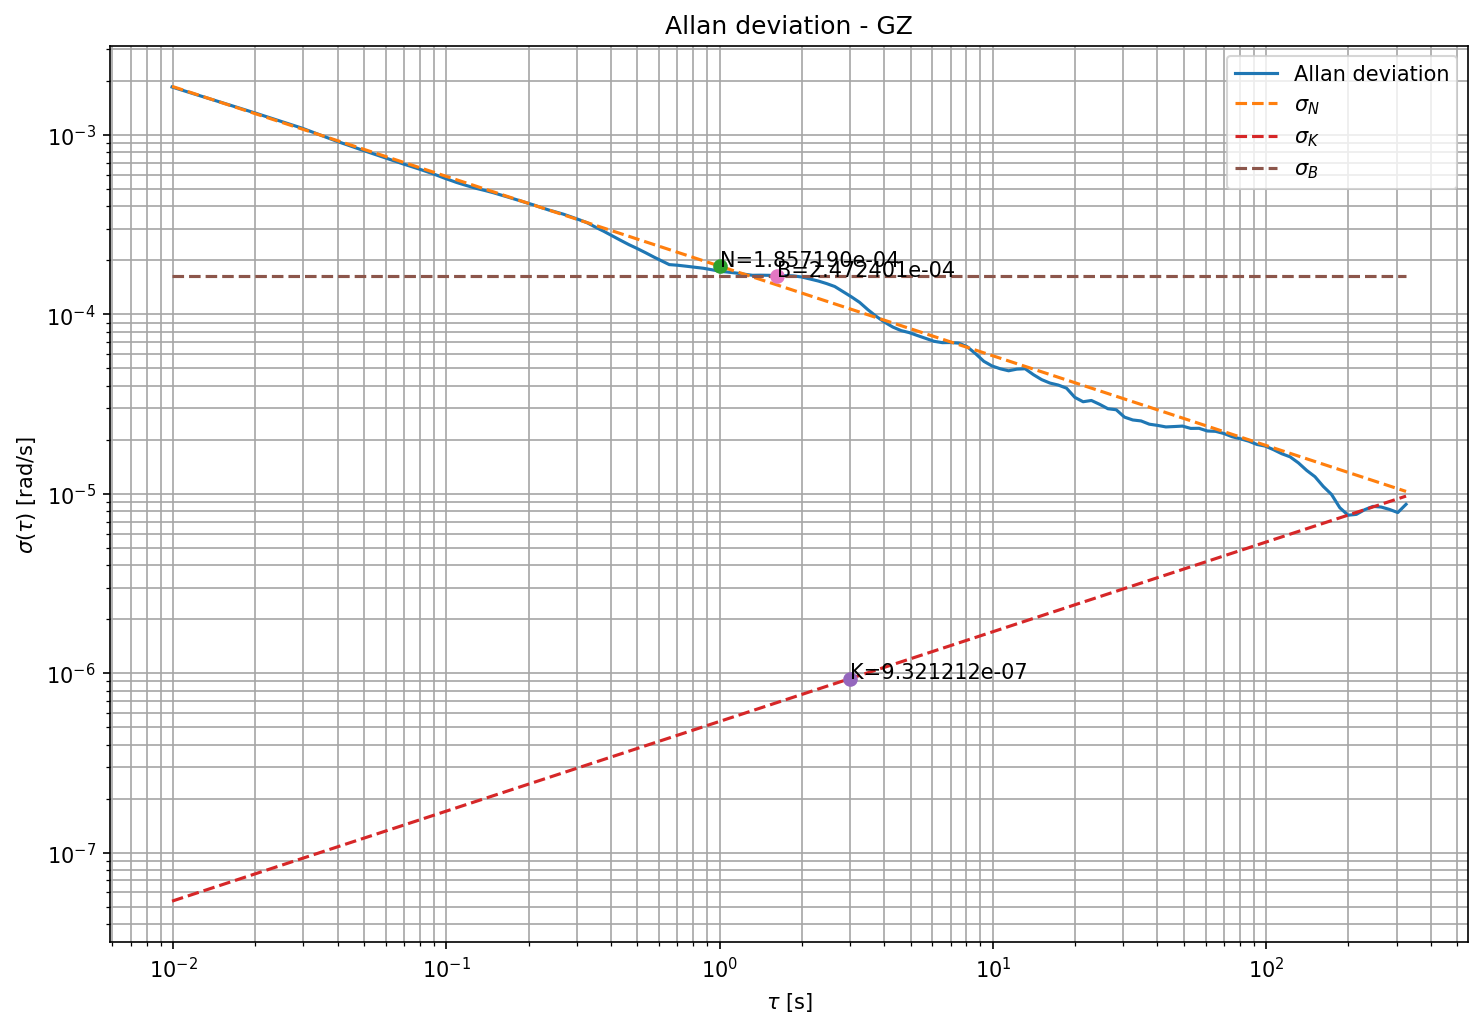
\includegraphics[width=0.88\textwidth]{images/gz_allan.png}
    \caption{Curva de desviación de Allan correspondiente al eje \(z\) del giróscopo durante el ensayo estático de una hora.}
    \label{fig:allan_gz_anexo}
\end{figure}
% \input{annexes/B_anex}

\end{document}